\documentclass[a4paper,10pt]{article}
\usepackage{graphicx}
\usepackage{epsfig}
\usepackage{subfigure}

% type user-defined commands here

\setlength{\topmargin}      {-15mm}  %  25-5 = 20mm
\setlength{\oddsidemargin}  {-5mm}  % rhs page inner margin = 25+10mm
\setlength{\evensidemargin} {0mm}   % lhs page outer margin = 25mm
\setlength{\textwidth}      {170mm} % 35 + 150 + 25 = 210mm
\setlength{\textheight}     {250mm} %

% Title Page

\title{
    An L1d module for improved description of light diaphragm rupture.
}
\author{
    Mechanical Engineering Report 2006/X\\
    Daniel F. Potter\\Centre for Hypersonics\\The University of Queensland.
}
\date{$21^{st}$ of December 2006}

\begin{document}
\maketitle

\begin{abstract}
L1d has been found to introduce errors at the contact surface when simulating diaphragm rupture, most notably for high-enthalpy expansion tube conditions.  In some instances the discontinuities in the flow properties are so large that the simulation is prematurely terminated.  It is proposed the wave-pattern for the time-steps immediately following light diaphragm rupture be described by the idealised Riemann solution, thus providing L1d with more acceptable boundary conditions at the interface.  An exact Riemann solver capable of handling an arbitrary, time-independent equation of state has been written for this purpose.  In this report the Riemann sub-problem module is described in detail and applied to a number of test cases to assess its effectiveness in mitigating contact surface discontinuities.  While considerable improvement is observed for both the ideal shock tube tests cases invetigated, the module is found to be less effective for application to high-enthalpy expansion tube conditions due to the inviscid nature of the Riemann solution.
\end{abstract}

\newpage

\tableofcontents

\newpage

\section{Introduction}

L1d is a computer program developed by the `Compressible Flow CFD' group at the University of Queensland for simulating the gas-dynamic processes within transient-flow facilities, such as free-piston shock and expansion tubes, and light-gas guns \cite{jacobs_98b}.  The quasi-one-dimensional, Lagrangian description of the flow allows the interaction between gas slugs, point masses and tube walls to be easily described.
\par \medskip
Diaphragms are modelled in L1d as fixed-wall boundary conditions that can be `triggered' by exceeding a user specified pressure difference between the two adjacent gas slugs.  Once triggered, the fixed-wall boundary conditions typically stay in place for small period of time to replicate the inertial influence of the diaphragm on the flow, and then are removed to allow the adjacent gas slugs to interact.  This method of modelling diaphragms is refered to as the hold-time model, and adequately captures the physical processes for most conditions. 
\par \medskip
L1d is extensively used by experimentalists for simulating the high-pressure sections upstream of the light-secondary diaphragm in expansion tubes.  Expansion tubes utilise the total enthalpy multiplication mechanism of an unsteady expansion of the test gas to achieve higher velocities and total pressures whilst minimising freestream dissociation \cite{morgan_chapter}.  The transient solution just upstream of the diaphragm can then be used as an inflow boundary condition for a more detailed axisymmetric Navier-Stokes simulation of the low pressure acceleration tube \cite{jacobs_94}.  Expansion tube conditions typically generate very strong secondary shocks travelling at superorbital speeds of up to 12km/s through low pressure accelerator gas.  L1d has difficulty accurately capturing the rapid expansion of stagnated test gas upstream of the contact surface immediately after diaphragm rupture for such conditions.  Errors in the conserved quantities caused by this rapid expansion allow `glitches' at the contact surface to propogate in time through the solution.  In some extreme cases these glitches generate such unrealistic flow states that the simulation is prematurely terminated.
\par \medskip
As L1d forms an important role in the experimental-computational cycle of ground-based testing, a solution to this problem is required.  It is proposed the flow development for the time-steps immediately following light diaphragm rupture be described by idealised wave theory.  This amounts to solving the Riemann problem for the flow states across the diaphragm, and using the solution as a new boundary condition that L1d can more easily handle.

\section{Problem description}

\emph{Figure \ref{fig:ref_profile:a}} illustrates the typical density profile in L1d surrounding a light secondary diaphragm just prior to rupture.  The incident shock has reflected off the diaphragm and travelled upstream, stagnating the incoming test gas.  The initial shock system is driven by these stagnation conditions on the upstream side of the diaphragm and the low pressure accelerator gas at room temperature on the downstream side.  The Lagrangian distribution of the cells in L1d is also shown to illustrate the discretisation of the gas slugs surrounding the diaphragm.

\par \medskip

A sketch of the idealised wave-pattern a few microseconds after diaphragm rupture is illustrated in \emph{Figure \ref{fig:ref_profile:b}}.  This classical wave-pattern consists of an unsteady expansion of the stagnated test gas anchored at the original diaphragm location, driving a strong shock through the low pressure accelerator gas.  The test gas is expanded isentropically through the rarefaction wave to its final state just upstream of the contact surface. The unsteady expansion and shock wave are coupled by the requirement of constant pressure and velocity across the contact surface.  The Riemann sub-problem  (RSP) procedure relies on the assumption that for a sufficiently small elapsed time since rupture, the rarefaction wave tail will not have reached the reflected shock, and the stagnated test gas acts as an infinite reservoir.

\begin{figure}
\centering
\subfigure[Flow conditions surrounding secondary diaphragm at $t = t_{rupture}$] % caption for subfigure a
{
    \label{fig:ref_profile:a}
    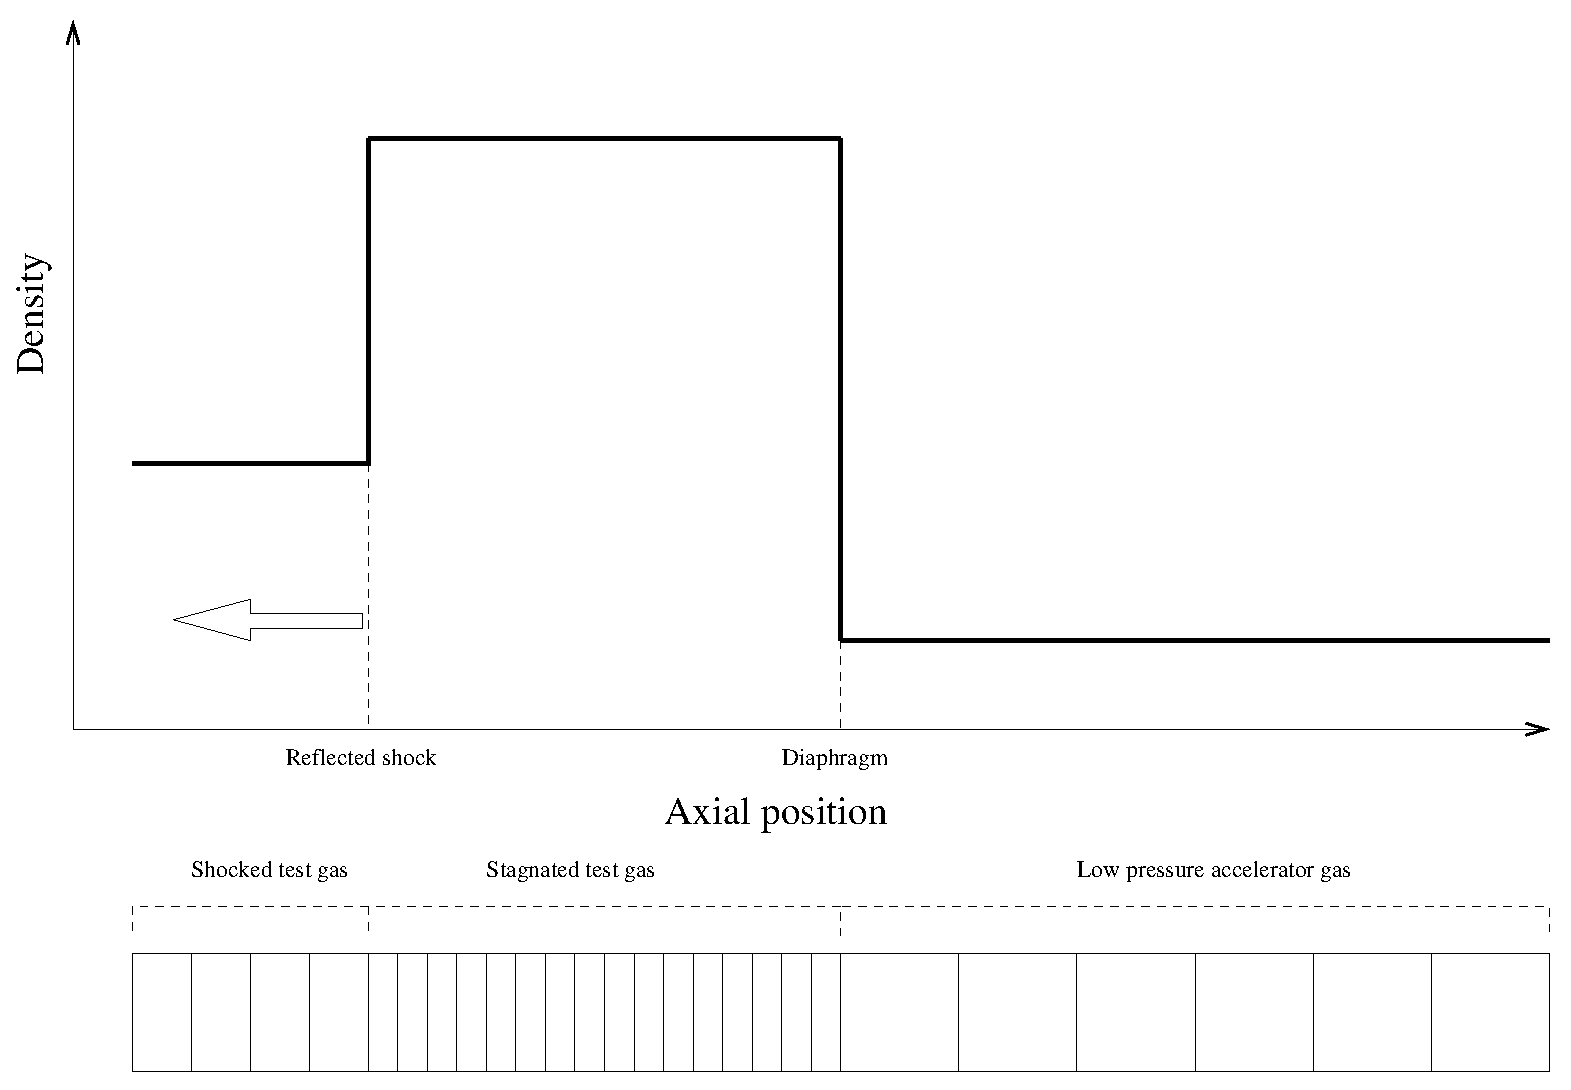
\includegraphics[scale=0.6]{figs/rsp_lagrange.eps}
} \hspace{1cm}
\subfigure[Flow conditions surrounding secondary diaphragm at $t = t_{rupture} + \Delta t$] % caption for subfigure b
{
    \label{fig:ref_profile:b}
    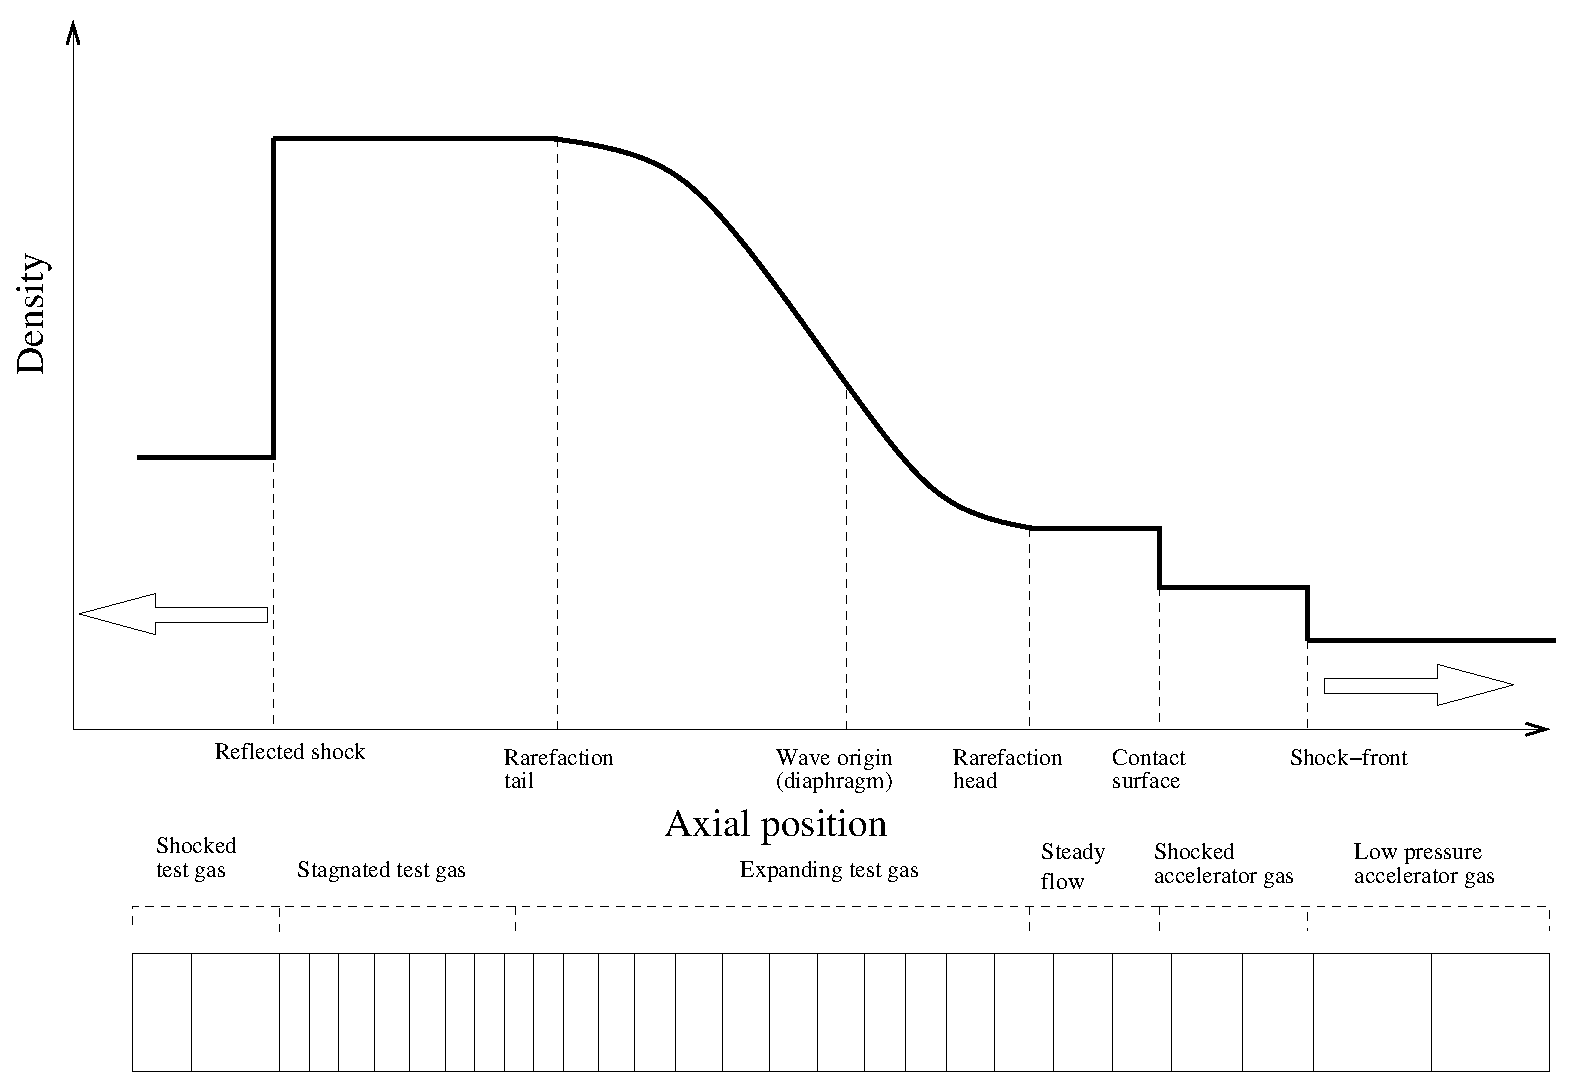
\includegraphics[scale=0.6]{figs/rsp_lagrange_final.eps}
} \caption{Typical density profiles and Lagrangian cell distributions for a hold-time model implemented in L1d}
\label{fig:ref_profile} % caption for the whole figure
\end{figure}

\par \medskip

In usual operation the wave-pattern will form in the L1d solution indirectly through the discretised, Lagrangian description of the gas slugs.  For the time-steps immediately following diaphragm rupture, however, the expansion-shock system is confined to a handful of cells either side of the diaphragm.  In attempting to describe the sudden expansion of the test gas at rupture with such low cell resolution, unphysical conditions are generated at at the contact surface that propogate in time through the solution.

\subsection{The hold-time model and diaphragm rupture in L1d}

The inertial influence of the diaphragm on the flow is accounted for in L1d using a simple hold-time model.  Although the severity of the hold-time model has been shown to overpredict the freestream dissociation in the test flow\cite{bakos,wilson}, it is however a convenient tool for estimating a light diaphragms influence on the flow development.  Petrie-Repar \cite{petrie} compared experimental static pressure traces just upstream of a light diaphragm with that obtained using a hold-time model within a quasi-one-dimensional finite-volume code, \emph{Figure \ref{fig:petrie_holdtime}}.  Although the predicted reflected shock strength is higher than that obtained experimentally, the general behaviour of the pressure trace is well described by the hold-time model.

\begin{figure}
\centering
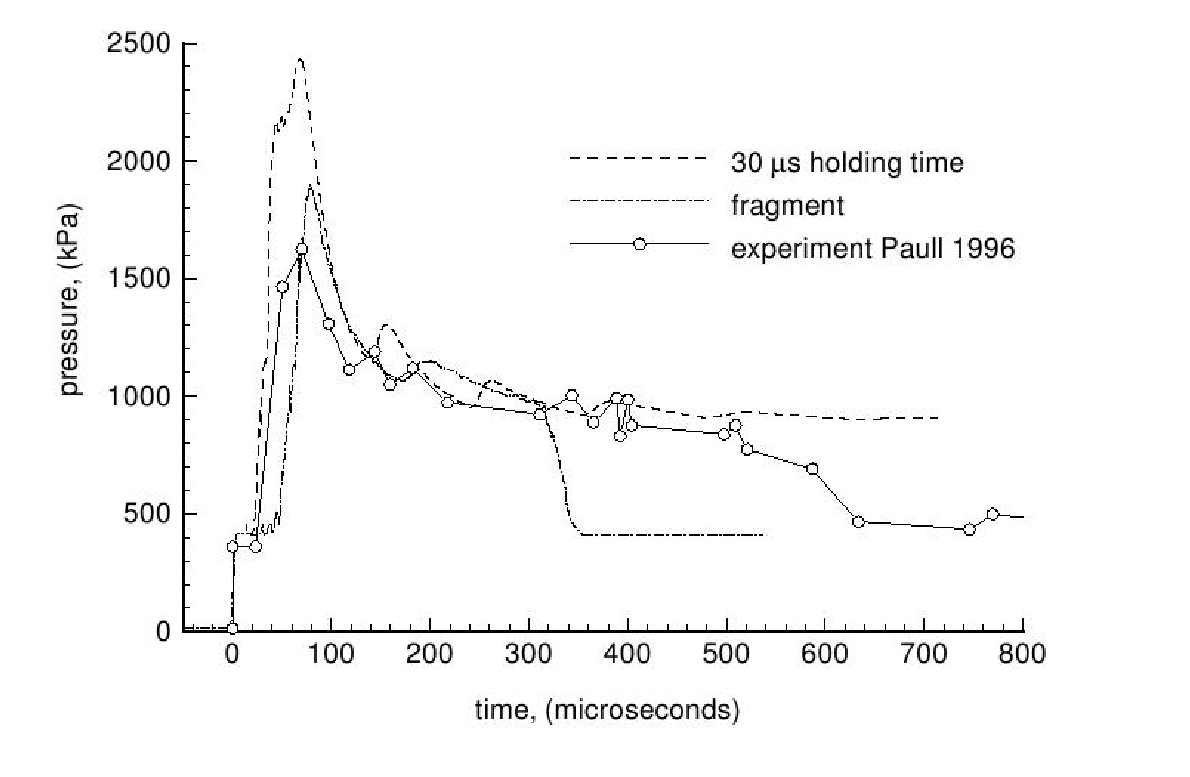
\includegraphics[scale=0.85]{figs/petrie_holdtime.eps}
\caption{Comparision of both a hold-time and a fragmentation model with experimental data of static pressure just upstream of a light diaphragm during rupture.  The incident shock has a velocity of 5.9km/s and the diaphragm thickness is $127\mu m$\cite{petrie}}.
\label{fig:petrie_holdtime}
\end{figure}

\par \medskip

The fixed wall assumption of the hold-time model followed by the instantaneous removal of the diaphragm leads to an excessive initial expansion rate of the upstream gas.  Following the derivation of Bakos and Morgan \cite{bakos}, the pressure history of a particle that enters the expansion fan at time $t_{0}$ after the
creation of the reflected shock for the hold time model can be expressed as

\par

\begin{equation}
\frac{p}{p_{0}} = \left ( \frac{t}{t_{0}} \right ) ^{ \frac{-2 \gamma }{ \gamma + 1 }} \label{hold_time}
\end{equation}

where $p_{0}$ is the pressure upstream of the diaphragm.  The expansion rate of a particle
immediately adjacent to the diaphragm for a sufficiently large
hold time can be found by differentiating the expression with
respect to time and setting $t=t_{0}$, \emph{Eq. \ref{eq:ht_diff}}.

\begin{equation}
\left ( \frac{dp}{d_{t}} \right )_{t=t_{0}} = -\frac{2 \gamma p_{0}}{t_{0}(\gamma + 1)} \label{eq:ht_diff}
\end{equation}

By setting $t_{0}=0$, it is revealed that an infinite initial
expansion rate exists for the hold time model where an ideal gas
is considered.  It must be noted that this derivation neglects both real gas effects and the resistance to the expansion provided by the accelerator gas.  In reality the downstream motion of the diaphragm, analogous to that of a piston, relaxes the initial rate of expansion.  The high initial expansion rate in L1d at rupture leads to the exchange of energy and momentum being overpredicted at the interface, and the cells bounding the contact surface being incorrectly discribed (see \emph{Appendix \ref{appendix_A}} for a detailed explanation of how the erroneous flux terms occur).

\par \medskip

A diagramatic representation of the contact surface errors are shown in \emph{Figure \ref{fig:cs_error}}.  A large temperature spike is induced on the upstream edge of shocked accelerator gas slug, and the temperature jump at the interface is smeared on the downstream edge.  The reciprocal effect on density is observed, with a large density drop just downstream of the contact surface and smearing on the upstream side.  Discontuities in both pressure and velocity are also introduced at the contact surface, corresponding to the misallocation of momentum at the interface.


\begin{figure}[ht]
\centering
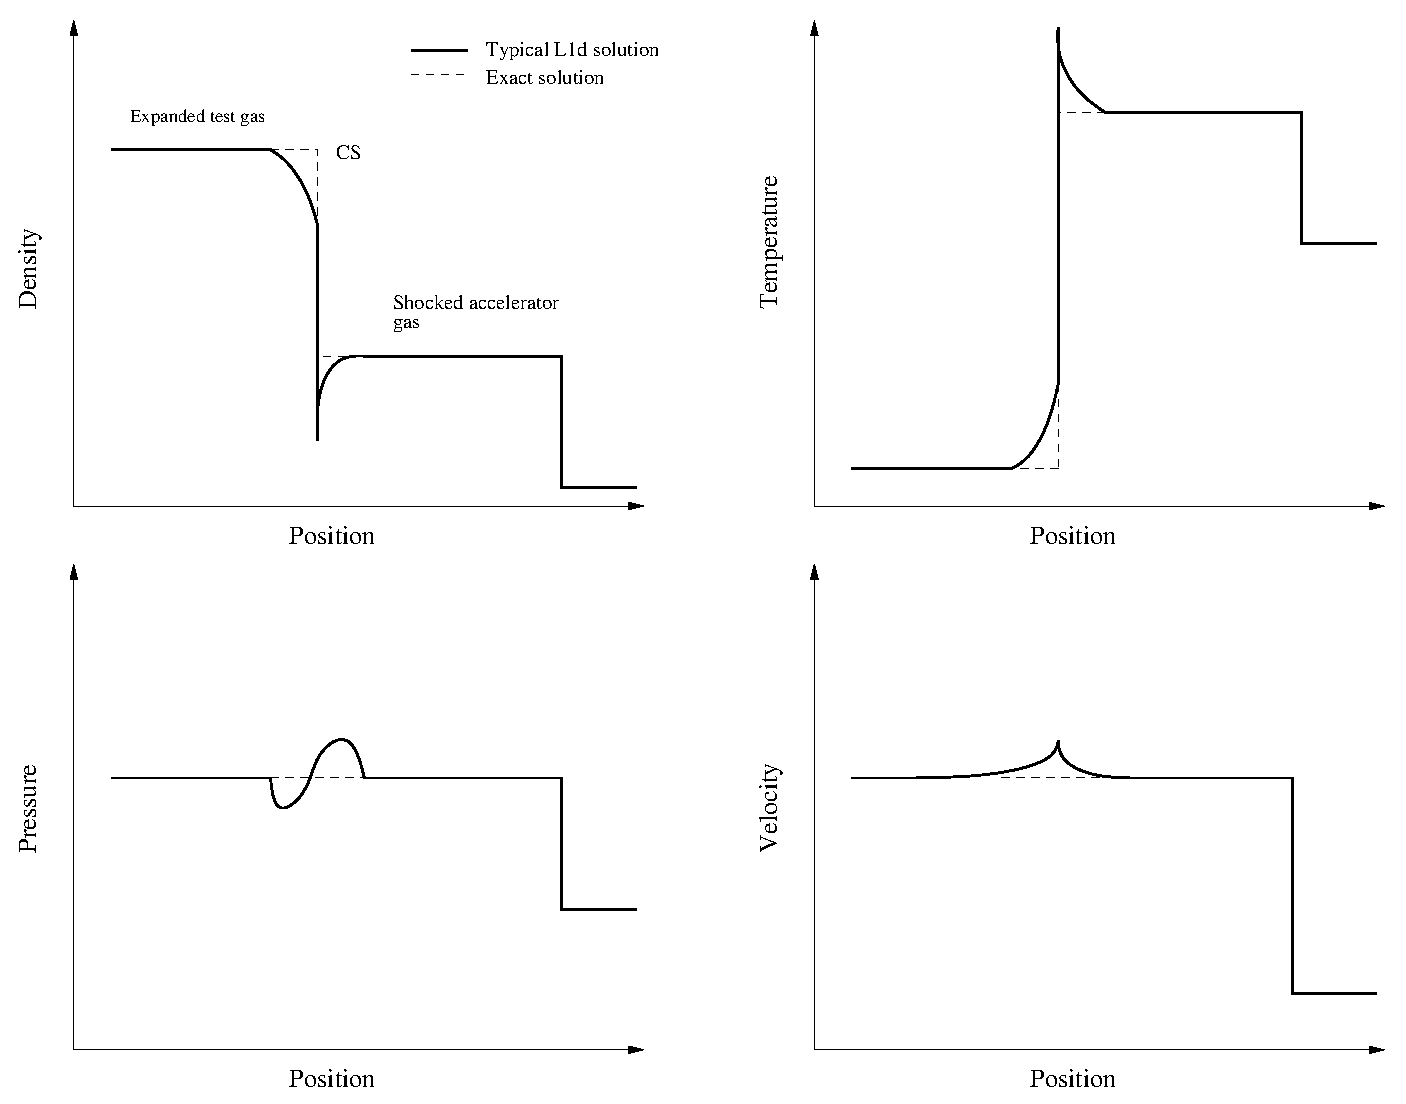
\includegraphics[scale=0.7]{figs/cs_error.eps}
\caption{Typical L1d flow profiles surrounding the contact surface shortly after diaphragm rupture}
\label{fig:cs_error}
\end{figure}

\par \medskip

For a number of high-enthalpy conditions conducted in the \emph{X} family of expansion tubes at the University of Queensland, the spike in temperature following light diaphragm rupture in L1d is so great that it exceeds the maximum allowable value of the equilibrium gas model.  Although the CEA provided look-up-tables are only considered accurate at temperatures less than $2 \times 10^{4}$ K \cite{gordon}, extrapolation to higher temperatures is required to capture the energy stored thermally for shocked gas slugs in equilibrium.  The initial temperature spike, however, can be significantly higher than the expected value.  The L1d simulation of an 11 km/s Jupiter gas condition conducted in the \emph{X2} facility in 2005, for example, resulted in an initial temperature spike in the shocked accelerator slug of almost $2 \times 10^{5}$ K \cite{my_ug_thesis}.  The equilibrium gas model cannot handle such unrealistic temperatures and the simulation terminates prematurely.

\par \medskip

The Riemann sub-problem module aims to describe the expansion and shock system evolving from the rupture of a light diaphragm using idealised wave-theory, thereby more accurately capturing the conditions at the contact surface.  As the contact surface errors are generated in the first few timesteps following rupture, the idealised solution need only be applied for the first few microseconds.  For such a short duration it is reasonable to assume the idealised solution will be sufficiently accurate, however high-enthalpy conditions may suffer from neglecting viscous effects in this small window of time.

\begin{figure}[hc]
\centering
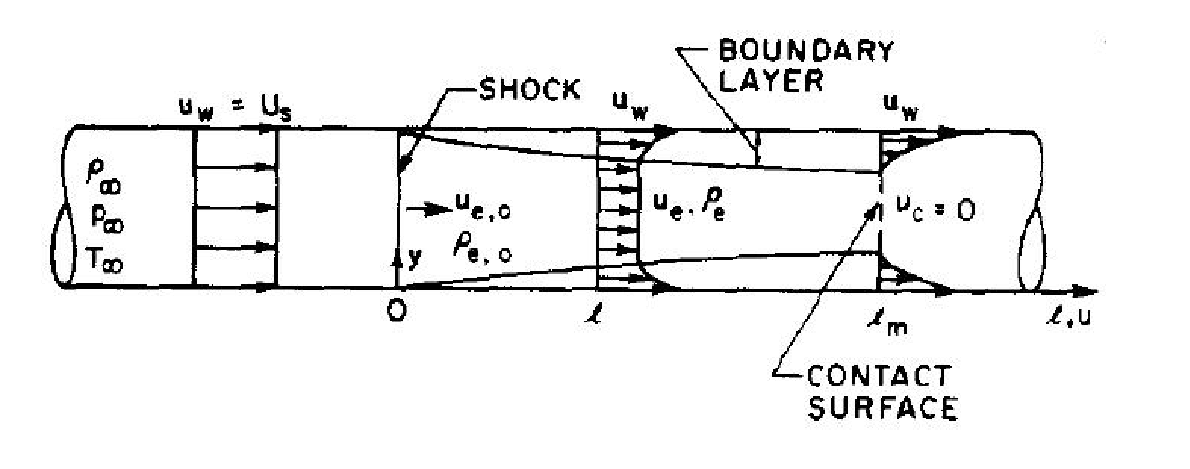
\includegraphics[scale=0.6]{figs/mirels_fig2.eps}
\caption{Flow between shock and contact surface in shock-stationary coordinate system in the Mirels analysis}
\label{fig:mirels_fig2}
\end{figure}

\subsection{Viscous effects}

The Riemann solution is idealised in that viscous effects are not considered.  Shock tube problems are inherently two-dimensional, in that the viscous interacton of the gas slugs with the tube walls can significantly influence the flow development and test gas conditions.  The classic shock tube flow development theory of Mirels predicts shock attenuation due to boundary layer mass entrainment \cite{mirels_63}.  The mass removal from the shocked gas slug to the boundary layer causes the shock to decelerate and the contact surface to accelerate asymptotically to an equilibrium separation distance, \emph{Figure \ref{fig:mirels_fig2}}.

\par \medskip

Con Doolan \cite{doolan} extended the viscous effects module in L1d to apply the Mirel's analysis on a cell-by-cell basis, thereby improving the description of the contact surface \cite{jacobs_98b}.  Although the Riemann solution is inviscid, the mass removal and attenuation induced by viscous interactions should not be substantial given the requirement of low $\Delta t_{RSP}$ values to ensure the assumption of an infinite reservoir is maintained.  A particularly severe condition, however, may not be able to be described inviscidly even for the shortest patching windows.  Indeed this was a problem with the faster expansion tube conditions investigated in \emph{Section 4}.


\subsection{The Riemann patching window}

The user must select a value for the Riemann patching window, $ \Delta t_{RSP} $, prior to running the simulation.  The quality of the resulting solution is strongly infuenced by the selection of an appropriate value for $ \Delta t_{RSP} $.  Selecting too low a value and the wave-pattern will be discretised over too few cells, usually on the shock side, resulting in a poor description of the flow upstream of the contact surface.  Selecting too high a value for $ \Delta t_{RSP} $ and the tail of the rarefaction wave will have caught up to the reflected shock, contradicting the assumption of an infinite reservoir driving the shock.

\par \medskip

The selected $ \Delta t_{RSP} $ for each diaphragm in a simulation is specified by the user in the diaphragm string of the Python input file.  Specifying a hold-time of $ 10.0 \mu s$ with a Riemann patching window of $ 0.5 \mu s$ would be done as below:

\par \medskip

\begin{small}
\begin{verbatim}
             diaphragm = Diaphragm(x0=8.234, p_burst=45.0e3, is_burst=0, dt_hold=10.e-6,
                                   dt_blend=0.0, dx_blend=0.0, RSP_dt=0.5e-6)
\end{verbatim}
\end{small}

\par \medskip

A good rule of thumb when selecting an appropriate value for $ \Delta t_{RSP} $ is to consider the number of cells, $n_{cells}$, traversed by the shock in this time,

\begin{equation}
n_{cells} = \frac{U_{s} \Delta t_{rsp}}{\Delta x_{cell, av}} \label{eq:rsp_dt}
\end{equation}

where $U_{s}$ is the shock speed and $\Delta x_{cell}$ is the average cell length in the accelerator gas slug.  Usual practice is to cluster these cells towards the diaphragm, therefore this relationship provides a conservative estimate for the number of cells.  Incorporating at least ten cells in the shock front has been found to give sufficient resolution for the shock-front to be well described.  As the stagnated test gas is of considerably higher density, the number of cells included in the rarefaction wave will invariably be sufficient for good resolution on the upstream side.  The sensitivity of the patched L1d solution to the selected $ \Delta t_{RSP} $ value is assessed for a number of test cases in \emph{Section \ref{testcases}}.

\subsection{The Riemann sub-problem procedure}

A flow chart describing the implementation of the RSP procedure within L1d is displayed in \emph{Figure \ref{fig:RSP_flow_chart}}.  Both L1d and the the RSP module are written in the \emph{c++} programming language.

\par \medskip

The RSP module is activated in L1d when a positive, non-zero value for $\Delta t_{RSP}$ is specified in the respective diaphragm class by the user.  For each of these diaphragms that will perform the RSP procedure at rupture, the required memory is allocated prior to the main integration loop in the L1d preamble.  The simulation starts, and at some time $t_{trig}$ the diaphragm is triggered at the arrival of the incident shock.  Where the diaphragm is usually held in place for the user specified hold-time, $\Delta t_{hold}$, the hold-time is now extended by the patching window to $\Delta t_{hold} + \Delta t_{RSP}$.  This enables L1d to continue simulating the evolution of the reflected shock while the RSP module waits for the new augmented hold-time to elapse.  During the time-step at which the simulation time first exceeds $t_{trig} + \Delta t_{hold} + \Delta t_{RSP}$, the RSP procedure is conducted.  The RSP procedure consists of five main steps as illustrated in \emph{Figure \ref{fig:RSP_flow_chart}}.

\begin{figure}[hcb]
\centering
\includegraphics[scale=0.8]{figs/RSP_flow_chart.eps}
\caption{Flow chart describing the implementation of the RSP procedure in L1d}
\label{fig:RSP_flow_chart}
\end{figure}

\par \medskip

The RSP procedure is initialised by solving for the extent of the region to be considered in the Riemann solution.  Although the stagnated test gas upstream of the diaphragm should theoretically be uniform, slight perturbations do exist.  As such the left and right flow states used to solve the wave-pattern are iterated for by averaging over the distance predicted by a perfect gas Riemann solver.  The left extent is dictated by the displacement of the rarefaction tail in the time $\Delta t_{RSP}$, and the right extent by that of the shock wave.  When a converged solution is found, the exact Riemann solver is used to accurately determine the wave-pattern.  This solution is then discretised into many points so it can be stored in an array to be used for interpolation.  If a converged solution is not found within five iterations, the initialisation procedure returns a failure and the RSP procedure is terminated.  Most conditions converge in two iterations.

\par \medskip

Once the Riemann solution for the wave-pattern has been solved for and stored as a set of discrete points, the solution can be patched into the L1d solution.  As the Lagrangian framework of L1d considers each cell to be a control mass, the cells within the wave-patterns region of influence must be moved and resized such that the average cell density matches that corresonding to the Riemann solution at the new cell centre.  The axial distribution and sizing of the cells is solely dictated by the density profile; once finalised, the rest of the flow properties can be interpolated from the discretised solution.

\par \medskip

Care must be taken during the patching procedure to ensure discontinuities are not introduced at either extremity of the wave-pattern.  These discontinuities occur through the inexact patching of the discretised Riemann solution into the L1d solution, and the unrealistic squashing or expansion of the bounding cells.  A check is performed to locate any such cells, and the wave-pattern adjusted appropriately to improve the solution.  For discontinuities adjacent to the rarefaction tail the entire wave-pattern is shifted to bring the density inline with the bounding cells.  This global shift of the pattern is small relative to the global length scale, as hundreds of cells are usually incorporated in the rarefaction wave.  Discontinuities ahead of the shock front are improved by spreading the shock-front over a number of cells, \emph{Figure \ref{fig:shock_alteration}}.

\begin{figure}
\centering
\subfigure[Shock extension] % caption for subfigure a
{
    \label{fig:shock_extension}
    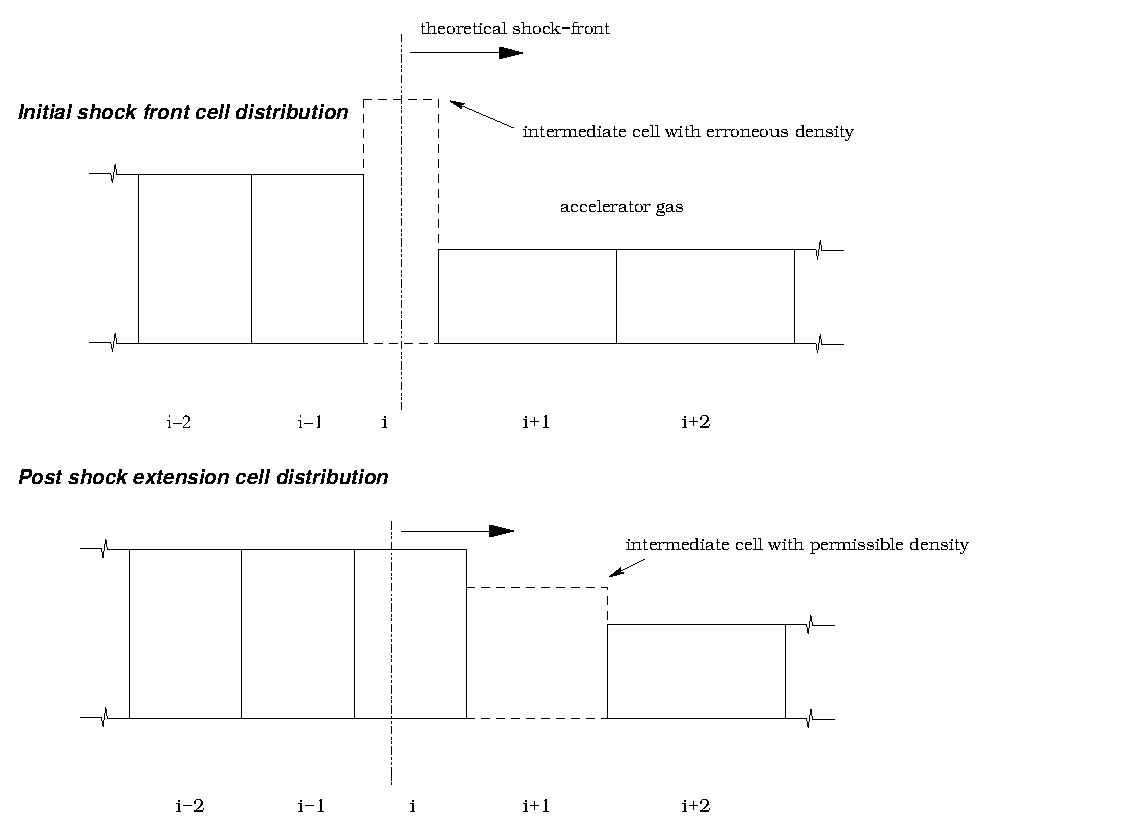
\includegraphics[scale=0.47]{figs/shock_extension.eps}
} \hspace{-1cm}
\subfigure[Shock retraction] % caption for subfigure b
{
    \label{fig:shock_retraction}
    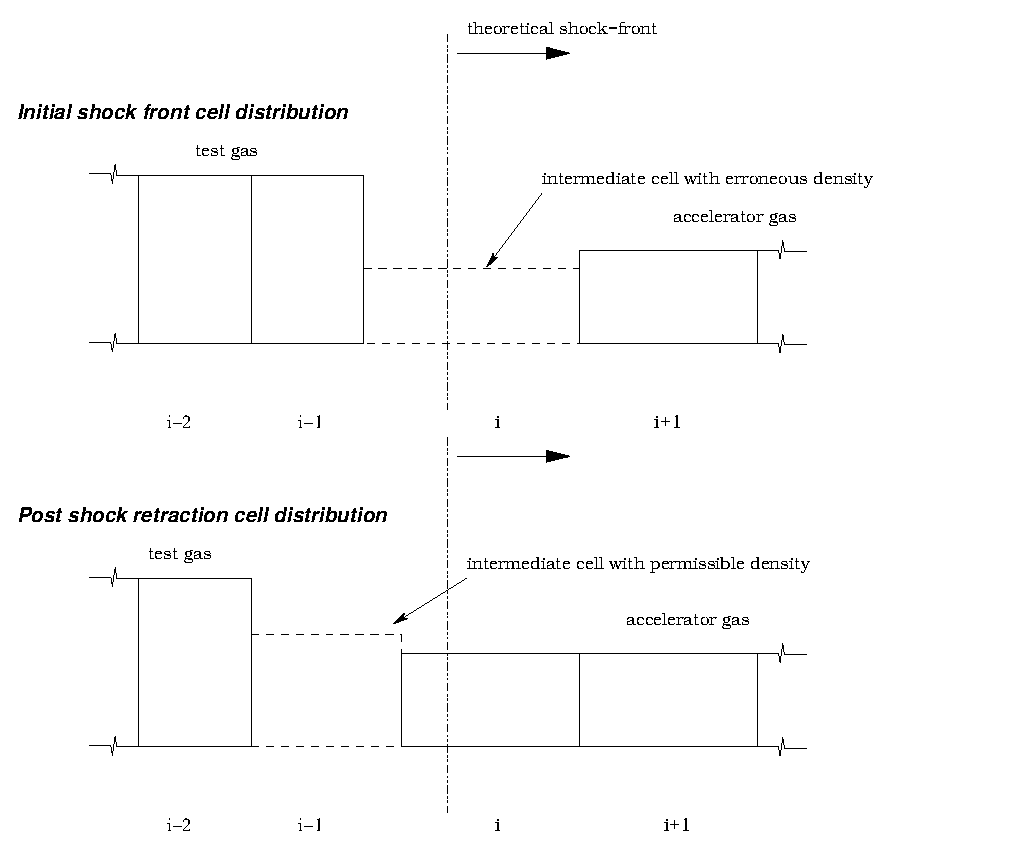
\includegraphics[scale=0.47]{figs/shock_retraction.eps}
} \caption{Improvement of erroneous bounding cells through alteration of shock front}
\label{fig:shock_alteration} % caption for the whole figure
\end{figure}

\par \medskip

Given that all steps of the RSP procedure have been performed successfully, the procedure is concluded by freeing all allocated memory, removing the fixed-wall diaphragm and exchanging the boundary condition information between the two slugs.  L1d then once more resumes responsibility for the cells included in the RSP procedure.

\section{An Exact Riemann Solver}

An exact solution to the unsteady expansion and shock wave system
emanating from a light diaphragm following its
rupture is required.  The instance of two separate gas slugs of
arbitrary thermodynamic state and velocity separated by an
interface is the classical Riemann problem, first introduced into
computational fluid dynamics by Godunov through his special
finite-difference methods for solving unsteady inviscid gas flows\cite{gottlieb}.  Solutions to the Riemann problem involve
determining the combination of waves that exist, their velocities
and flow properties of the evolved regions between the waves for a
specified time step.

\par \medskip

\begin{figure}[hbt]
\centering
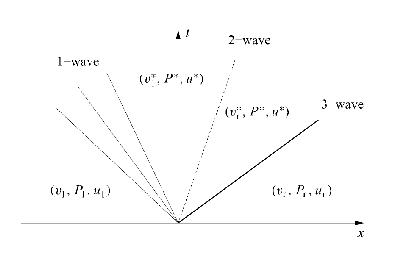
\includegraphics[scale=1.9]{figs/quart_riem.eps}
\caption{Riemann problem for the Euler equations of gasdynamics (Quartapelle, 2003)}
\label{fig:quart_riem}
\end{figure}

\emph{Figure \ref{fig:quart_riem}} illustrates the four states considered for the Riemann problem of an arbitrary wave-pattern.  The one-dimension Riemann invariants through a rarefaction wave
moving left or right can be expressed as:

\begin{eqnarray}
\psi_{1}^{\pm} &=& s \label{rare_inv1} \\
\psi_{2}^{\pm} &=& v \mp \int^{\rho^{*}} \rho^{-1} a ( \rho, s) d \rho \label{rare_inv2}
\end{eqnarray}

\emph{Eq. \ref{rare_inv1}} is required as the rarefaction wave is
an isentropic process, while \emph{Eq. \ref{rare_inv2}} specifies
the velocity change through the wave for a given final density, $
\rho^{*} $.  The one-dimension Riemann invariants across the
contact surface are based on the fundamental principle of the
Riemann problem, that the internal velocity and pressure is
constant on either side of the interface, \emph{Eq. \ref{cs_inv1}}
and \emph{Eq. \ref{cs_inv2}}.

\begin{eqnarray}
\psi_{1}^{\pm} &=& v \label{cs_inv1} \\
\psi_{2}^{\pm} &=& p \label{cs_inv2}
\end{eqnarray}

The Rankine-Hugoniot relations govern the jump conditions across
the normal shock wave, \emph{Eq. \ref{rh_rel1}} through
\emph{\ref{rh_rel3}} in a shock centered frame of reference, where
$i=r,l$, $V_{i} = v_{i} - U_{s}$ and * denotes the shock processed
state.  $U_{s}$ is the actual shock velocity.

\begin{eqnarray}
\rho_{i} V_{i} &=& \rho_{i}^{*} V_{i}^{*} \label{rh_rel1} \\
p_{i} + \rho_{i} V_{i}^{2} &=& p_{i}^{*} + \rho_{i}^{*} V_{i}^{*}{}^{2} \label{rh_rel2} \\
h_{i} + \frac{V_{i}^{2}}{2} &=& h_{i}^{*} + \frac{V_{i}^{*}{}^{2}}{2} \label{rh_rel3}
\end{eqnarray}

A solution to the Riemann problem for a given initial state is
found where each of the jump relations relevant to the
predetermined wave-pattern, \emph{Eq. \ref{rare_inv1}} through
\emph{\ref{rh_rel3}}, are satisfied simultaneously.  An iterative
method is required whereby one of internal velocity or pressure is
varied until both of the contact surface invariants are satisfied,
and the rarefaction and shock jump relations used to define
the predicted internal states for each iteration.

\subsection{Perfect Gas Solution}

A perfect gas solution to the Riemann problem is useful for providing an accurate initial guess for the wave-pattern at hand.  The method proposed by Gottlieb and Groth \cite{gottlieb} has been selected due to its efficiency and robustness in
dealing with all possible wave-patterns.  The perfect gas Riemann problem is a relatively trivial problem as the wave-pattern can be evaluated \emph{a-priori} and the Riemann invariants are available as closed form expressions, as is the derivative of internal pressure with respect to velocity.

\par \medskip

\emph{Eq. \ref{shock_1}} through \emph{\ref{shock_4}} state the relevant equations for a left or right facing shock wave:

\par

\begin{eqnarray}
W_{i} &=& \frac{\gamma_{i} +1}{4} \frac{u_{*}-u_{i}}{a_{i}} \pm \left [ 1 + \left ( \frac{\gamma_{i} +1 }{4} \frac{u_{*}-u_{1}}{a_{1}} \right ) ^{2} \right] ^{1/2} \label{shock_1} \\
p_{i}^{*} &=& p_{1} + C_{i} ( u^{*} - u_{1} ) W_{i} \label{shock_2} \\
\frac{d p_{i}^{*}}{ d u_{i}^{*}} &=& \frac{2 C_{i} (W_{i})^{3}}{1+(W_{i})_{2}} \label{shock_3} \\
a_{i}^{*} &=& a_{i} \left [ \frac{ (\gamma_{i} + 1) + (\gamma_{i} - 1) p_{i}^{*} / p_{i} }{ (\gamma_{i} + 1) + (\gamma_{i} - 1) p_{i} / p_{i}^{*} } \right ] ^{1/2} \label{shock_4}
\end{eqnarray}

The parameter $C_{i}$ is equal to $\gamma_{i} p_{i} / a_{i} $ and evaluated before the iterative loop commences.  $W_{i}$ is the shock Mach number with respect to the unprocessed gas ahead of the shock.  For a left or right rarefaction wave the jump relations are:

\begin{eqnarray}
a_{i}^{*} &=& a_{i} \pm \frac{\gamma_{i} - 1}{2} (u^{*} - u_{i}) \label{rare_1} \\
p_{i}^{*} &=& p_{1} \left [ \frac{a_{i}^{*}}{a_{i}} \right ] ^{\frac{2 \gamma _{i} }{(\gamma_{i} -1) }} \label{rare_2} \\
\frac{d p_{i}^{*}}{ d u_{i}^{*}} &=& \pm \frac{p_{i}^{*}}{a_{i}^{*}} \label{rare_3}
\end{eqnarray}

An initial guess for the interior velocity can be evaluated according to \emph{Eq. \ref{pg_u_ig}}.

\begin{eqnarray}
u_{0}^{*} &=& \frac{ \widetilde{u}_{l} z + \widetilde{u}_{r}}{1+z} \label{pg_u_ig}
\end{eqnarray}

where

\begin{eqnarray}
\widetilde{u}_{l} &=& u_{l} + \frac{2}{\gamma_{l} - 1}a_{l} \label{u_left} \\
\widetilde{u}_{r} &=& u_{l} - \frac{2}{\gamma_{r} - 1}a_{r} \label{u_right} \\
z &=& \frac{ \gamma_{l}- 1 }{ \gamma_{r} - 1 } \frac{a_{r}}{a_{l}} \left [ \frac{p_{l}}{p_{r}} \right ] ^{ (\sigma - 1) / 2 \sigma } \label{z_uni} \\
\sigma &=& \left\{ \begin{array}{c} \gamma_{l}, p_{l} \geq p_{r} \\
\gamma_{r}, p_{l} < p_{r} \end{array} \right\} \label{sigma_riem}
\end{eqnarray}

 Once a converged interior velocity and pressure solution has been found, the wave velocities and interior flow states are computed.  For a shock wave the shock velocity $V_{i}$ is given by $u_{i} + a_{i} W_{i} $, and for a rarefaction have the velocity of the head given by $u_{i} \pm a_{i}$ and the tail by  $u_{i}^{*} \pm a_{i}^{*}$.  As the ratio of specific heats and the gas constant remain unchanged for perfect gas equations of state, the processed temperature and thus the gas state can be found by considering the definition of sonic velocity, $a^{2} = \gamma R T$.
\par
\medskip
The calculation of the respective wave speeds allows the flow states at an arbitrary time and position to be found, assuming the wave-pattern is allowed to propagate without hindrance for the time step given.  This is required in the context of the diaphragm rupture problem to solve for the flow states through the unsteady expansion fan for a specified time step.

\subsection{Arbitrary EOS Solution}

A variety of gas models are implemented in L1d, such as perfect gas mixtures, equilibrium gases via the use of CEA generated look-up-tables and finite-rate schemes \footnote{The use of finite-rate schemes in conjunction with the RSP module is currently not supported}.  A Riemann solver capable of handling an arbitrary equation of state is therefore required.  Saurel et al \cite{saurel} outlines such a procedure where the internal pressure is the iterative variable.  As an expression for the derivative of velocity with respect to pressure is not attainable for an arbitrary equation of state, the secant method is implemented for the iterative procedure:

\begin{equation}
p_{j+1}^{*} = p_{j}^{*} - f(p_{j}^{*}) \frac{p_{j}^{*} - p_{j-1}^{*}}{f(p_{j}^{*}) - f(p_{j-1}^{*})} \label{secant_method}
\end{equation}

where

\begin{equation}
f(p_{j}^{*}) = \frac{u_{l}(p_{j}^{*})}{u_{r}(p_{j}^{*})}-1 \label{f_zero}
\end{equation}

Convergence is deemed to occur when $f(p_{j+1}^{*}) < \epsilon $, where a tolerance $\epsilon$ of $1 \times 10^{-6}$ has been found to be sufficient for most cases.  The  initial guesses for the internal pressure required by the secant method are supplied by two pressures on either side of the solution obtained by the perfect gas procedure.  The wave-pattern is re-evaluated at each step of the iterative procedure, where a shock wave is deemed to exist where $ p_{i}^{*} > p_{i} $, a rarefaction wave where $ p_{i}^{*} < p_{i} $ and no wave where $ p_{i}^{*} = p_{i} $.  This is in contrast to the perfect gas Riemann problem where the wave-pattern is known \emph{a-priori} to the iterative procedure by considering the left and right flow states alone.
\par
\medskip

Where the jump relations reduce to direct expressions for a perfect gas equation of state, the generalised expressions need to be evaluated when considering a real gas.  The evaluation of the Riemann invariant integral, \emph{Eq. \ref{rare_inv2b}}, for a rarefaction wave along an isentropic path is responsible for the majority of the computational resolution required in solving the Riemann problem for an arbitrary equation of state.
\par

\begin{eqnarray}
v_{i}^{\pm} &=& v_{i} \mp \int^{\rho_{i}^{*}}_{\rho_{i}} \rho^{-1}
a ( \rho, s) d \rho \label{rare_inv2b}
\end{eqnarray}

Prior to the integral being numerically evaluated, the upper density bound $\rho_{i}^{*}$ must be found.  This is done by finding the intersection between the isobar and isentrope for the specified guess for internal pressure $p^{*}$ and the unprocessed gas state respectively.  This is equivalent to solving for the density in the following expression:

\begin{equation}
p^{*} - p (\rho,T_{s(\rho)}) = 0 \label{isos}
\end{equation}

It is necessary to step along the isentrope from the unprocessed state at $\rho_{i}$ until \emph{Eq. \ref{isos}} is satisfied.  The temperature after each density step is found via the following expression for the derivative of temperature with respect to density for constant entropy:

\begin{equation}
\left ( \frac{ \partial T }{ \partial \rho } \right )_{s} = \frac{T}{C_{v}\rho^{2}} \frac{1}{(\partial T / \partial p)_{\rho}} \label{isen}
\end{equation}

This isentrope stepping procedure requires the equation of state be evaluated at each step, proving computationally expensive for the number of steps required to achieve reasonable levels of accuracy.  Once the density $\rho^{*}$ has been found the integral in the rarefaction Riemann invariant, \emph{Eq. \ref{rare_inv2b}}, can be evaluated to solve for the internal velocity.
\par
\medskip

The Rankine-Hugoniot equations that form the jump relations for the shock wave need to be evaluated iteratively as the enthalpy of the processed state, $h_{i}^{*}$, is not known \emph{a-priori}.  \emph{Eq. \ref{rh_rel1}} through \emph{\ref{rh_rel3}} are combined to form an expression for the enthalpy change from the fluid dynamics perspective, \emph{Eq. \ref{enthalpy1}}, while a second expression is obtained via the thermodynamic definition of enthalpy, \emph{Eq. \ref{enthalpy2}}.
\par
\begin{eqnarray}
\left ( h_{i}^{*} - h_{i} \right )_{RH} &=& \frac{V_{i}^{2}}{2} - \frac{1}{2} \left ( \frac{ p_{i} - p_{i}^{*} + \rho_{i} V_{i}^{2}}{\rho_{i} V_{i}} \right ) ^{2} \label{enthalpy1} \\
\left ( h_{i}^{*} - h_{i} \right )_{thermo} &=& \left ( e^{*} + \frac{p^{*}}{\rho^{*}} \right )_{i} - \left ( e + \frac{p}{\rho} \right )_{i} \label{enthalpy2}
\end{eqnarray}

Thus for a given guess for internal pressure the internal velocity can be found by equating the two expressions and iteratively solving the following zero value problem:

\begin{equation}
0=1-\frac{\left ( h_{i}^{*} - h_{i} \right )_{RH}}{\left ( h_{i}^{*} - h_{i} \right )_{thermo}} \label{shock_energy}
\end{equation}

Again the secant method is used as analytical expressions for the exact derivatives are not available.  Once a converged solution for the internal pressure and velocity is found, the flow states through any rarefaction waves that have been shown to exist are calculated by steppnig through the unsteady expansion to the contact surface.  

\subsection{Code Description}

A numerical procedure consisting of both perfect gas and real gas exact Riemann solvers has been formulated in the $c++$ programming language.  The procedures outlined by Gottlieb and Groth \cite{gottlieb} and Saurel et al \cite{saurel} respectively have been adapted for computational efficiency and to suit the form of the thermochemistry functions available. The code makes use of the flexible equations of state provided in the \emph{Gas Models 2} library to minimise the expensive evaluation of thermodynamic properties, such as the isentropic derivatives of temperature.  The generic \emph{L\_flow\_state} structure as defined in \emph{l1d.hh} is implemented to simplify interaction with the L1d data structures. 

\par
\medskip

\emph{Table \ref{table:numerical_methods}} summarises the numerical methods implemented for various parts of the program, and the nominal values of the relevant parameters used for the proceeding test cases.  Simulation time must also taken into consideration as high resolution procedures for frequently called operations, such as the stepping procedure for solving the rarefaction isobar-isentrope intercept, can increase the solution time considerably.  The values listed here have been shown to provide a good compromise between efficiency and accuracy\footnote{See reference \cite{my_ug_thesis} for a complete discussion and validation of the exact Riemann solver}.

\begin{table}[ht]
\begin{center}  % put inside center environment
\begin{tabular*}{1.0\textwidth}%
     {@{\extracolsep{\fill}}cccc}
\hline \hline \textbf{Procedure} & \textbf{Numerical Method} & \textbf{Parameters} & \textbf{Parameter value} \\
\hline
\\
Perfect gas iterative & Newton's method & Convergence tol., $\epsilon$ & $1 \times 10^{-10} $ \\
loop \\
\\
Arbitrary EOS & Secant method & Convergence tol., $\epsilon$ & $1 \times 10^{-6} $ \\
iterative loop \\
\\
Isobar/isentrope intercept & 1$^{st}$ order stepping & Steps of $ \Delta \rho $ & $1:10^{3}$ \\
$ 0 = p^{*} - p (\rho,T_{s(\rho)}) $
\\
\\
shock speed iteration & Secant method & Convergence tol., $\epsilon$ & $1 \times 10^{-10} $ \\
$0=1-\frac{ \Delta h_{RH}(U_{s})}{ \Delta h _{thermo}(U_{s})}$
\\
\\
\hline
\end{tabular*}
\caption{Numerical methods implemented in exact Riemann solver procedure} \label{table:numerical_methods}
\end{center}
\end{table}

\section{Test Cases}
\label{testcases}

The RSP module has been applied to a variety of test cases to demonstrate its effectiveness in improving the flow description following the rupture of a light diaphragm.  Firstly an ideal shock tube is considered, characterised by a perfect gas equation of state and inviscid gas elements.  The RSP procedure is then applied to three real conditions conducted in the X2 expansion tube, with an equilibrium equation of state and the inclusion of viscous effects.

\subsection{Ideal shock tube}

The benefits of implementing the RSP module in L1d are most effectively conveyed by considering an ideal shock tube.  A direct comparision can be made between the standard L1d solution, the patched L1d solution and an exact analytical solution obtained from idealised wave theory.

\par \medskip

Two separate ideal shock tube conditions are considered; the classic Sod shock tube, and a higher enthalpy condition with a shock speed of approximately 4km/s.  Sod's ideal shock tube \cite{sod} is used extensively as a test case for compressible flow codes, and is an appropriate starting point for validating the RSP module in L1d.  As the motivation for the module was drawn from the inability of L1d to accurately capture the contact surface in high-enthalpy expansion tube conditions, a high-enthalpy ideal shock tube is also an appropriate test case.  \emph{Table \ref{table:ideal_cases}} details the conditions implemented for both of these test cases.  Viscous effects are not considered as a direct comparision with an analytical solution is desired.  The initial slugs are all 500mm in length.

\par \medskip

\begin{table}[tbh]
\begin{center}  % put inside center environment
\begin{tabular*}{0.8\textwidth}%
     {@{\extracolsep{\fill}}ccc}
\hline \hline  & \textbf{Sod shock tube} & \textbf{High-enthalpy shock tube} \\
\hline \textbf{\emph{LHS slug}} & PG air ($\gamma=1.4$) & PG air ($\gamma=1.4$) \\
$p_{L} (kPa)$     &         100.0         &           1000.0      \\
$T_{L} (K)$       &         348.4         &           5000.0      \\
$u_{L} (m/s)$     &           0           &             0         \\
$n_{cells,L}$     &         100           &            200        \\
\\
\textbf{\emph{RHS slug}} & PG air ($\gamma=1.4$) & PG air ($\gamma=1.4$)   \\
$p_{R} (kPa)$     &         10.0          &           0.01        \\
$T_{R} (K)$       &         278.7         &           300.0      \\
$u_{R} (m/s)$     &           0           &             0         \\
$n_{cells,R}$     &         100           &            200        \\
\hline
\end{tabular*}
\caption{L1d input parameters for ideal shock tube test cases} \label{table:ideal_cases}
\end{center}
\end{table}

\subsubsection{Sod shock tube}

As the Sod shock tube has a relatively low shock speed ($U_{s} \approx 500 m/s$), the Riemann patching window needs to be large in order to achieve sufficient cell resolution for the patched profile.  A duration of $50 \mu s$ is selected for $\Delta t_{RSP}$ as to allow the shock to traverse approimately ten cells in accordance with \emph{Eq. \ref{eq:rsp_dt}}.

\begin{figure}[h]
\centering
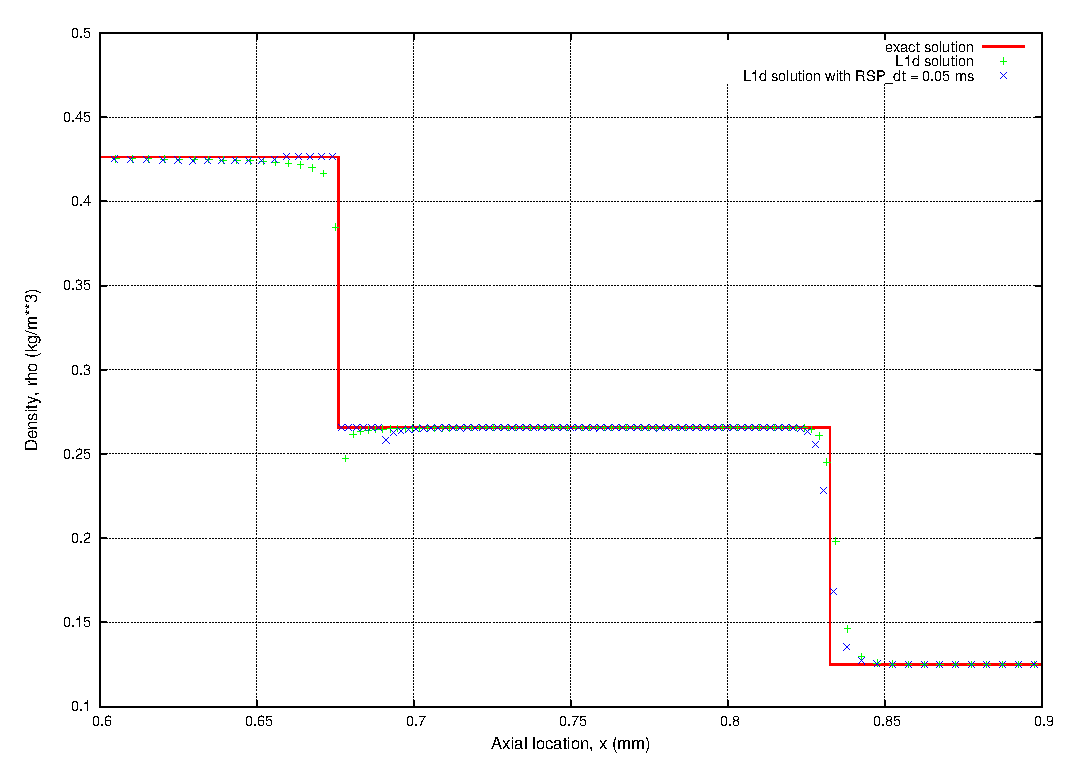
\includegraphics[scale=0.9]{figs/sod_density_detail.eps}
\caption{Density profile detail surrounding the contact surface for the Sod ideal shock tube 0.6 ms after diaphragm rupture}
\label{fig:sod_density} % caption for the whole figure
\end{figure}

\par \medskip

\emph{Table \ref{table:sod_rsp}} summarises the implementation of the RSP procedure for the Sod shock tube test case.  Sufficient cell resolution is achieved through the wave-pattern, with eight cells incorporated in the shock-front and thirteen in the expansion wave.  The calculated shock speed, internal pressure and internal velocity all agree to at least one significant figure with the accepted perfect gas solution to the Sod shock tube.  The cells adjacent to the ends of the rarefaction and shock waves assume allowable values on the first attempt, and therefore no global shift or alteration of the shock front is required.

\begin{table}[tbh]
\begin{center}  % put inside center environment
\begin{tabular*}{0.5\textwidth}%
     {@{\extracolsep{\fill}}cc}
\hline Patching window, $\Delta t_{RSP}$ & $50 \mu s$ \\
Shock-front cells, $n_{shock}$ & 8 \\
Rarefaction cells, $n_{rare}$ & 13 \\
Shock speed, $U_{s}$ & $554.1 m/s$ \\
Internal pressure, $p^{*}$ & $30.3 kPa$ \\
Internal velocity, $u^{*}$ & $293.3 m/s$ \\
Global shift, $\Delta x_{global}$ & - \\
Shock shift, $\Delta x_{shock}$ & - \\
\hline
\end{tabular*}
\caption{Summary of RSP procedure performed in L1d for the Sod shock tube test case} \label{table:sod_rsp}
\end{center}
\end{table}

\emph{Figure \ref{fig:sod_profiles}} compares the flow profiles 0.6 milliseconds after diaphragm rupture for Sod's ideal shock tube.  Detail of the density profile surrounding the contact surface is shown in \emph{Figure \ref{fig:sod_density}}.  Whilst only a slight reduction in the smearing of the tail and head of the rarefaction is observed, considerable improvement of the contact surface is evident.  The density discontinuity at the contact surface is resolved with little of the distortion shown in the standard L1d solution.  A slight perturbation is observed in the patched L1d solution just downstream of the contact surface.  This feature originates from the shock-front and diffuses upstream relative to the shock as the simulation progresses.  Considerable effort has been put into attempting to remove this feature from the patched solution.  It was found that the magnitude of the discontinuity can be minimised by selecting an optimal value for the Riemann patching window.

\begin{figure}[tbh]
  \begin{center}
    \mbox{
      \subfigure[Pressure]
      {
         \label{fig:sub:c}
         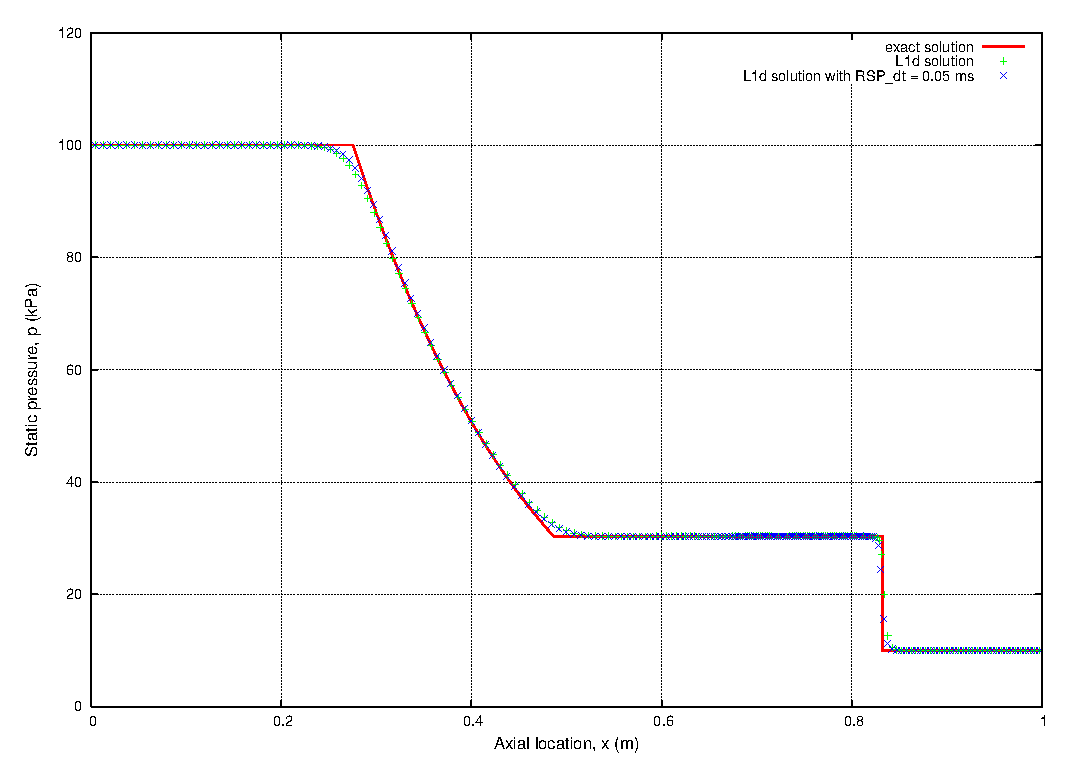
\includegraphics[scale=0.45]{figs/sod_pressure.eps}
      } \quad
      \subfigure[Temperature]
      {
         \label{fig:sub:d}
         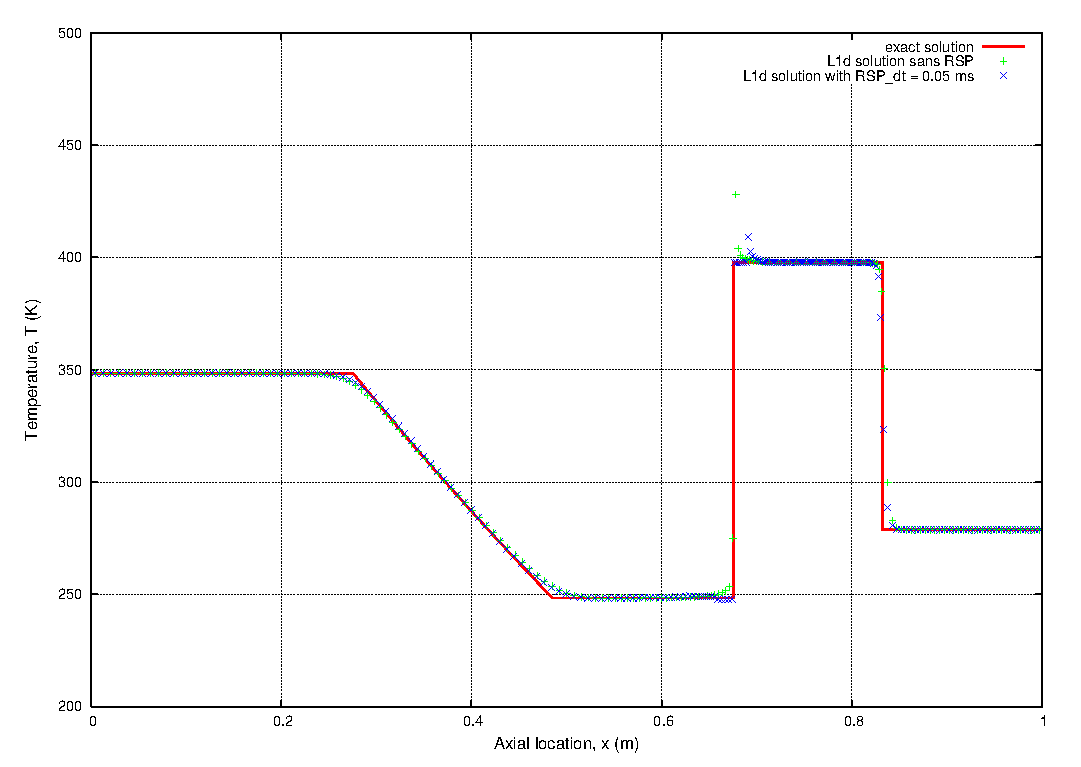
\includegraphics[scale=0.45]{figs/sod_temperature.eps}
      }
      }
    \mbox{
      \subfigure[Density]
      {
         \label{fig:sub:e}
         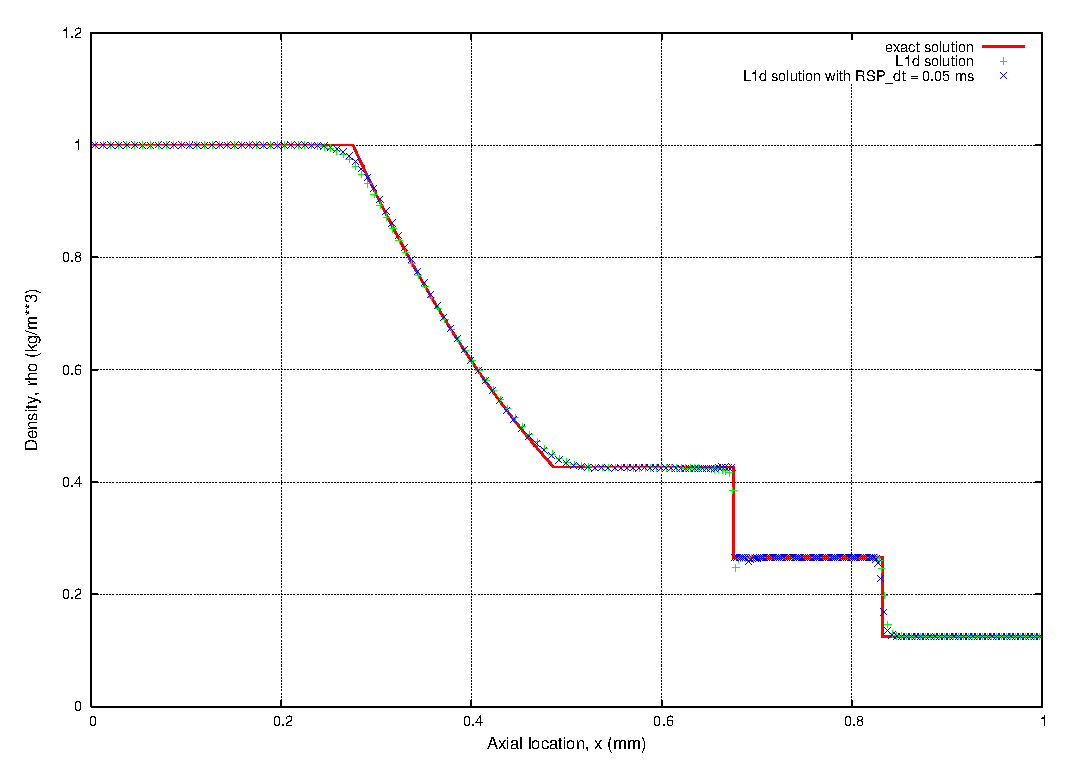
\includegraphics[scale=0.45]{figs/sod_density.eps}
      } \quad
      \subfigure[Velocity]
      {
         \label{fig:sub:f}
         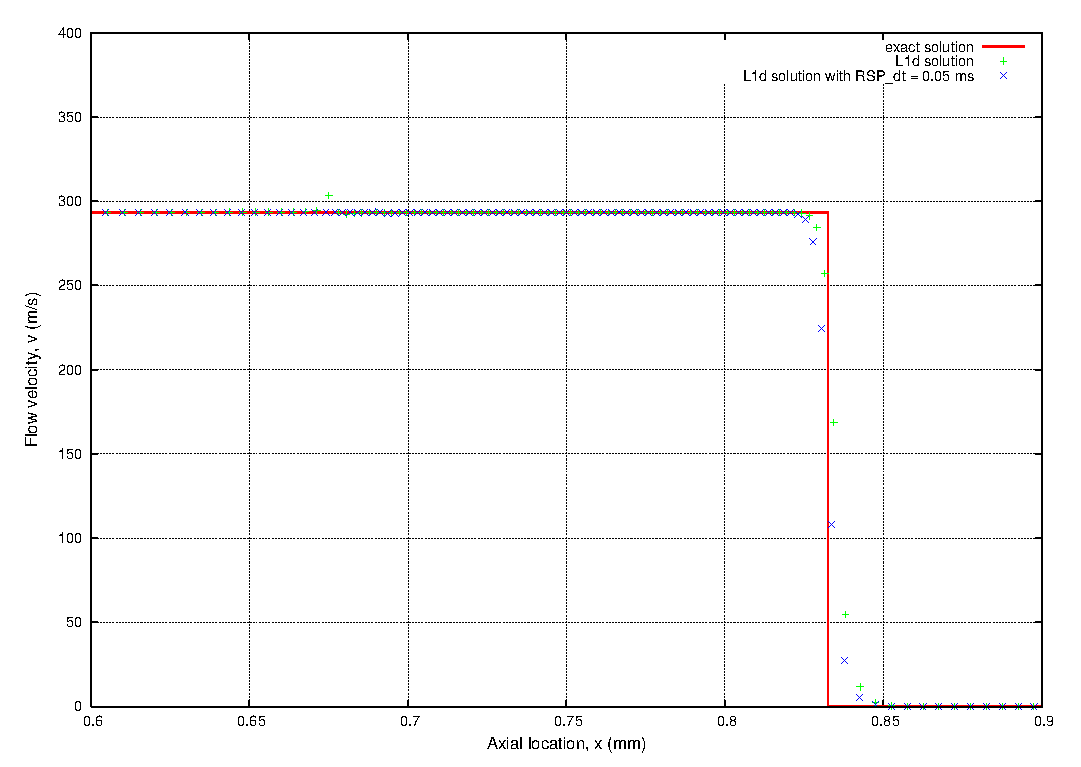
\includegraphics[scale=0.45]{figs/sod_velocity.eps}
      } 
      }
    \caption{Flow profiles for the Sod ideal shock tube 0.6 microseconds after diaphragm rupture}
    \label{fig:sod_profiles}
  \end{center}
\end{figure} 

\subsubsection{High-enthalpy ideal shock tube}

This high-enthalpy test case maintains the geometry and ideal assumptions of the Sod shock tube test case, whilst substanitally increasing the severity of the resultant shock (see \emph{Table \ref{table:ideal_cases}} for fill conditions).  As such the number of cells and clustering towards the diaphragm is increased to more effectively capture the initial expansion.  Again the patching window is selected such that approximately ten cells will be included in the shock front, giving a $\Delta t_{RSP}$ duration of $5 \mu s$.

\par \medskip

\begin{table}[hb]
\begin{center}  % put inside center environment
\begin{tabular*}{0.5\textwidth}%
     {@{\extracolsep{\fill}}cc}
\hline Patching window, $\Delta t_{RSP}$ & $5 \mu s$ \\
Shock-front cells, $n_{shock}$ & 10 \\
Rarefaction cells, $n_{rare}$ & 11 \\
Shock speed, $U_{s}$ & $3887.5 m/s$ \\
Internal pressure, $p^{*}$ & $14.6 kPa$ \\
Internal velocity, $u^{*}$ & $3213.7 m/s$ \\
Global shift, $\Delta x_{global}$ & - \\
Shock shift, $\Delta x_{shock}$ & - \\
\hline
\end{tabular*}
\caption{Summary of RSP procedure performed in L1d for the high-enthalpy ideal shock tube test case} \label{table:he_rsp}
\end{center}
\end{table}

\emph{Table \ref{table:he_rsp}} summarises the implementation of the RSP for the high-enthalpy ideal shock tube test case.  Again the anticipated resolution in the shock front is achieved and no alteration of the wave-pattern is required as the adjacent cells assume allowable values.  The calculated shock speed and internal conditions agree well with the values predicted by the perfect gas analytical solution.

\par \medskip

\begin{figure}[htbp]
  \begin{center}
    \mbox{
      \subfigure[Pressure]
      {
         \label{fig:sub:g}
         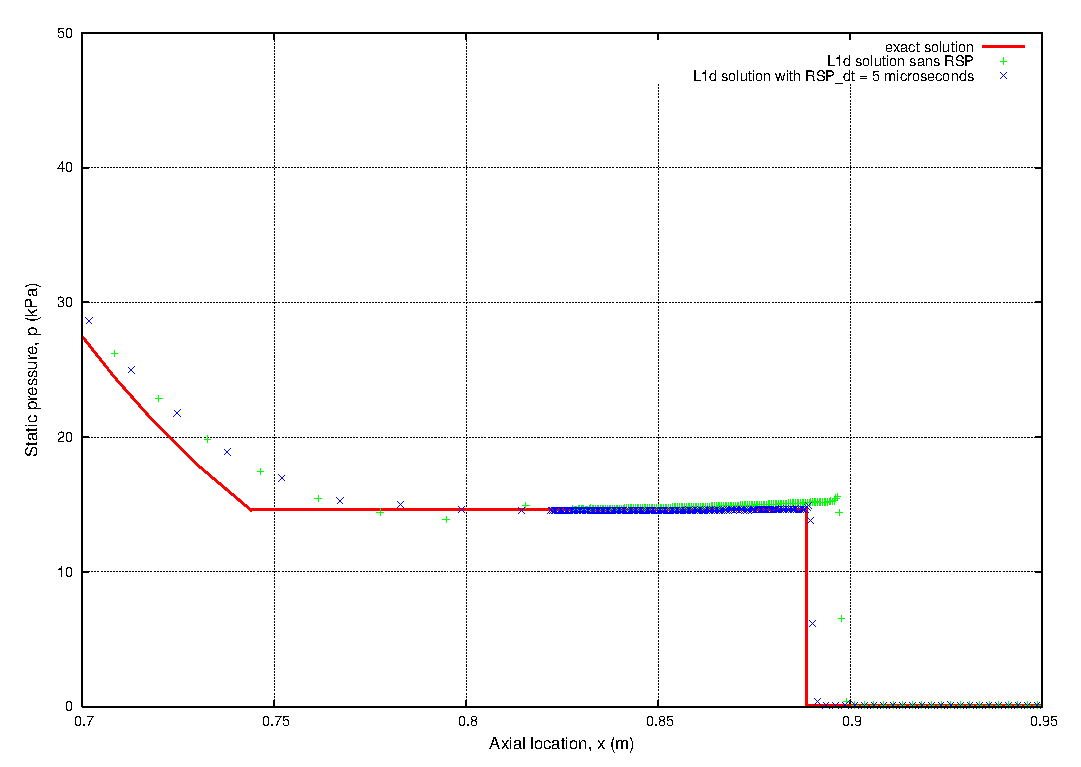
\includegraphics[scale=0.45]{figs/he_pressure_detail.eps}
      } \quad
      \subfigure[Temperature]
      {
         \label{fig:sub:h}
         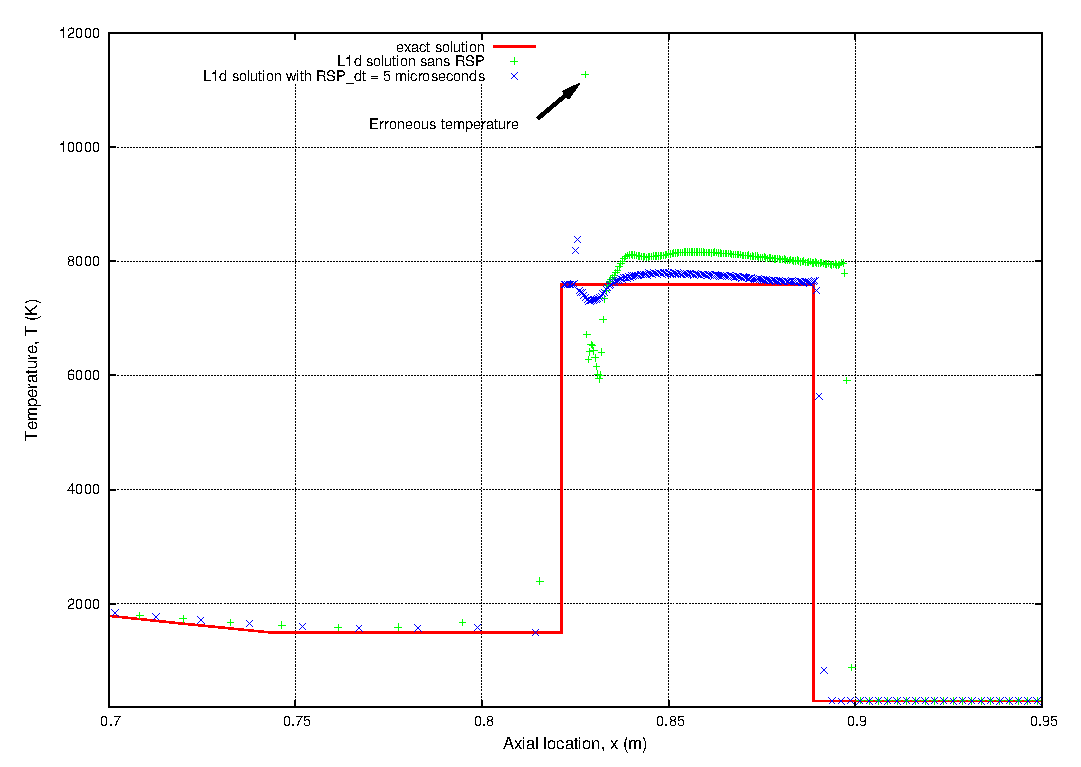
\includegraphics[scale=0.45]{figs/he_temperature_detail.eps}
      }
      }
    \mbox{
      \subfigure[Density]
      {
         \label{fig:sub:i}
         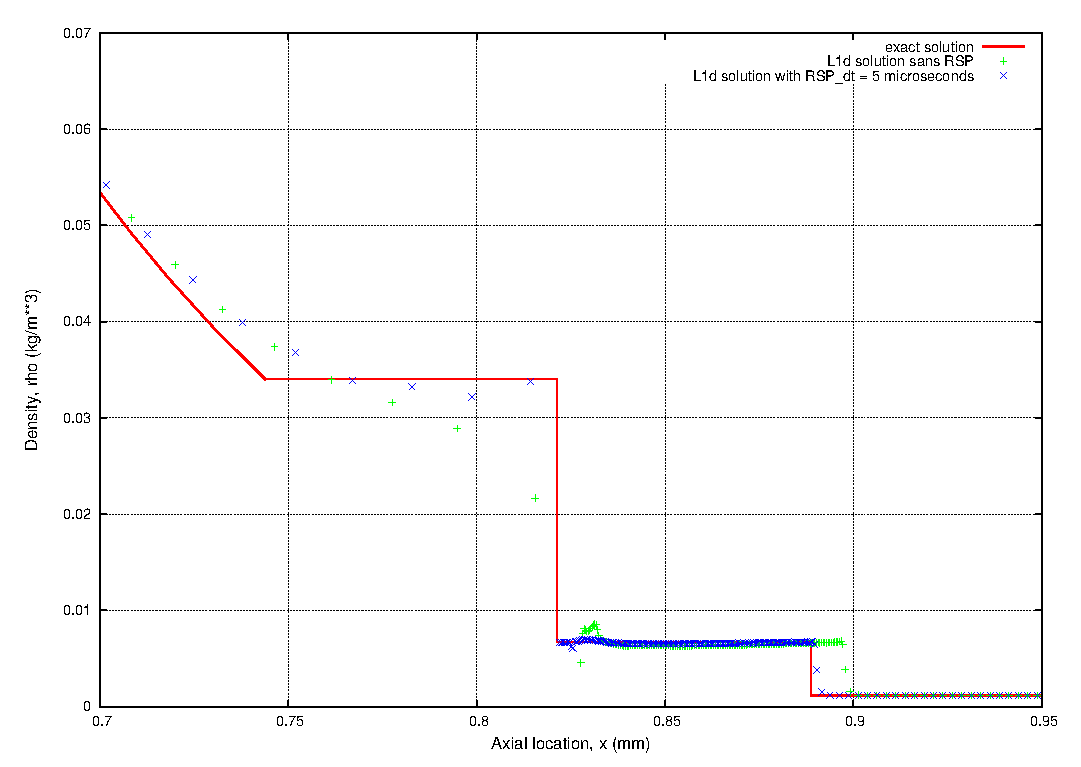
\includegraphics[scale=0.45]{figs/he_density_detail.eps}
      } \quad
      \subfigure[Velocity]
      {
         \label{fig:sub:j}
         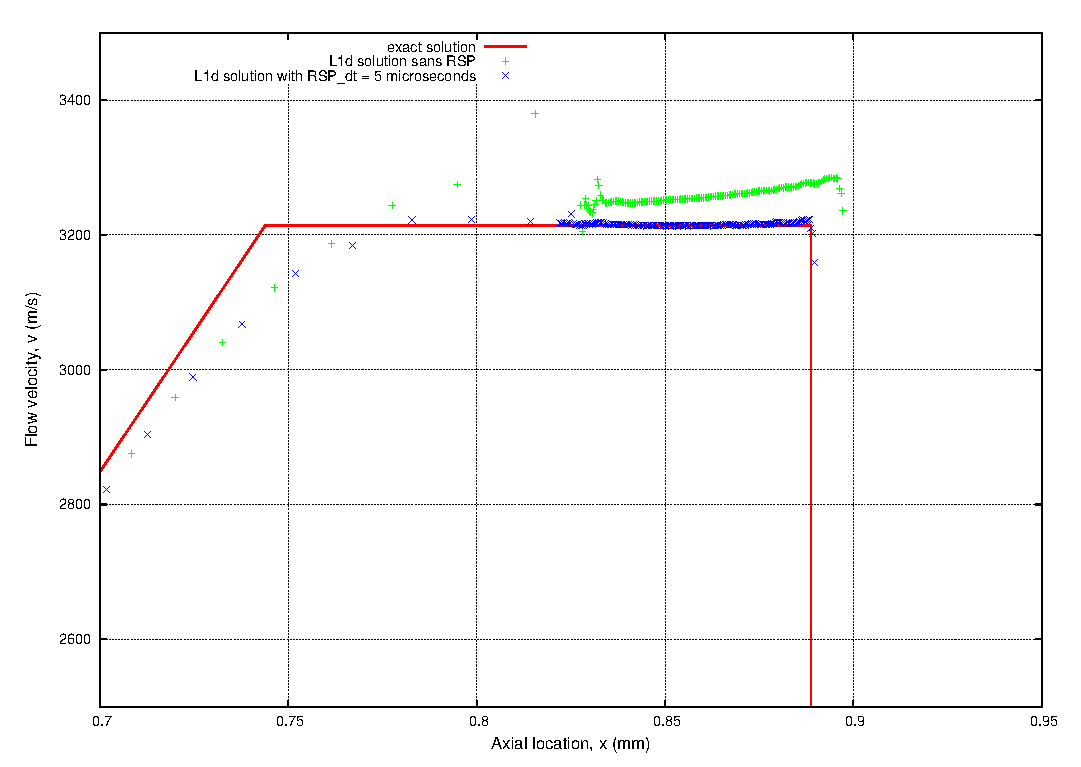
\includegraphics[scale=0.45]{figs/he_velocity_detail.eps}
      } 
      }
    \caption{Flow profiles for a high-enthalpy ideal shock tube 0.1 microseconds after diaphragm rupture}
    \label{fig:he_profiles}
  \end{center}
\end{figure}

\emph{Figure \ref{fig:he_profiles}} compares the flow profile detail surrounding the contact surface 0.1 milliseconds after diaphragm rupture.  The RSP module is seen to durastically improve the conformity of the L1d solution to the exact analytical solution.  The standard L1d solution notably over-predicts the location of the shock-front and fails to accurately capture the flow states either side of the contact surface.  The slug of fully expanded air upstream of the interface is poorly described, with density varying considerably in the predicted steady flow region.  A large discontinuity also exits just downstream of the interface, most notable by the erroneous temperature in \emph{Figure \ref{fig:sub:h}} which deviates by 40\% from the expected shocked gas temperature.

\par \medskip

In contrast, the patched L1d solution exhibits minimal distortion of the steady flow region and almost exactly captures the true location of the shock-front.  The temperature discontinuity observed in the standard solution is significantly reduced, with the maximum temperature deviation in the shock-front being less than 5\%.  Most importantly for the simulation of expansion tube conditions, the region of steady flow upstream of the contact surface is captured with greater accuracy.  This is most obvious in the density and velocity profiles with the patched solution agreeing well with the analytical solution.

\subsection{X2 expansion tube}

The X2 facility, as illustrated in \emph{Figure \ref{fig:x2_tube}}, is a free-piston expansion tube consisting of a reservoir, compression tube, shock tube and an accleration tube.  Current conditions burst a 1mm mild steel diaphragm at 15MPa, and can generate flows with total ethalpies up to approximately 100 MJ/kg.  Typical test times are around 100 $\mu s$ when operated in the expansion tube mode, and up to 200 $\mu s$ when operated as an expansion tunnel \footnote{For expansion tunnel operation, a Mach 9 full capture nozzle designed by Michael Scott \cite{scott} is used to expand the test flow at the end of the acceleration tube}.

\begin{figure}[h]
\centering
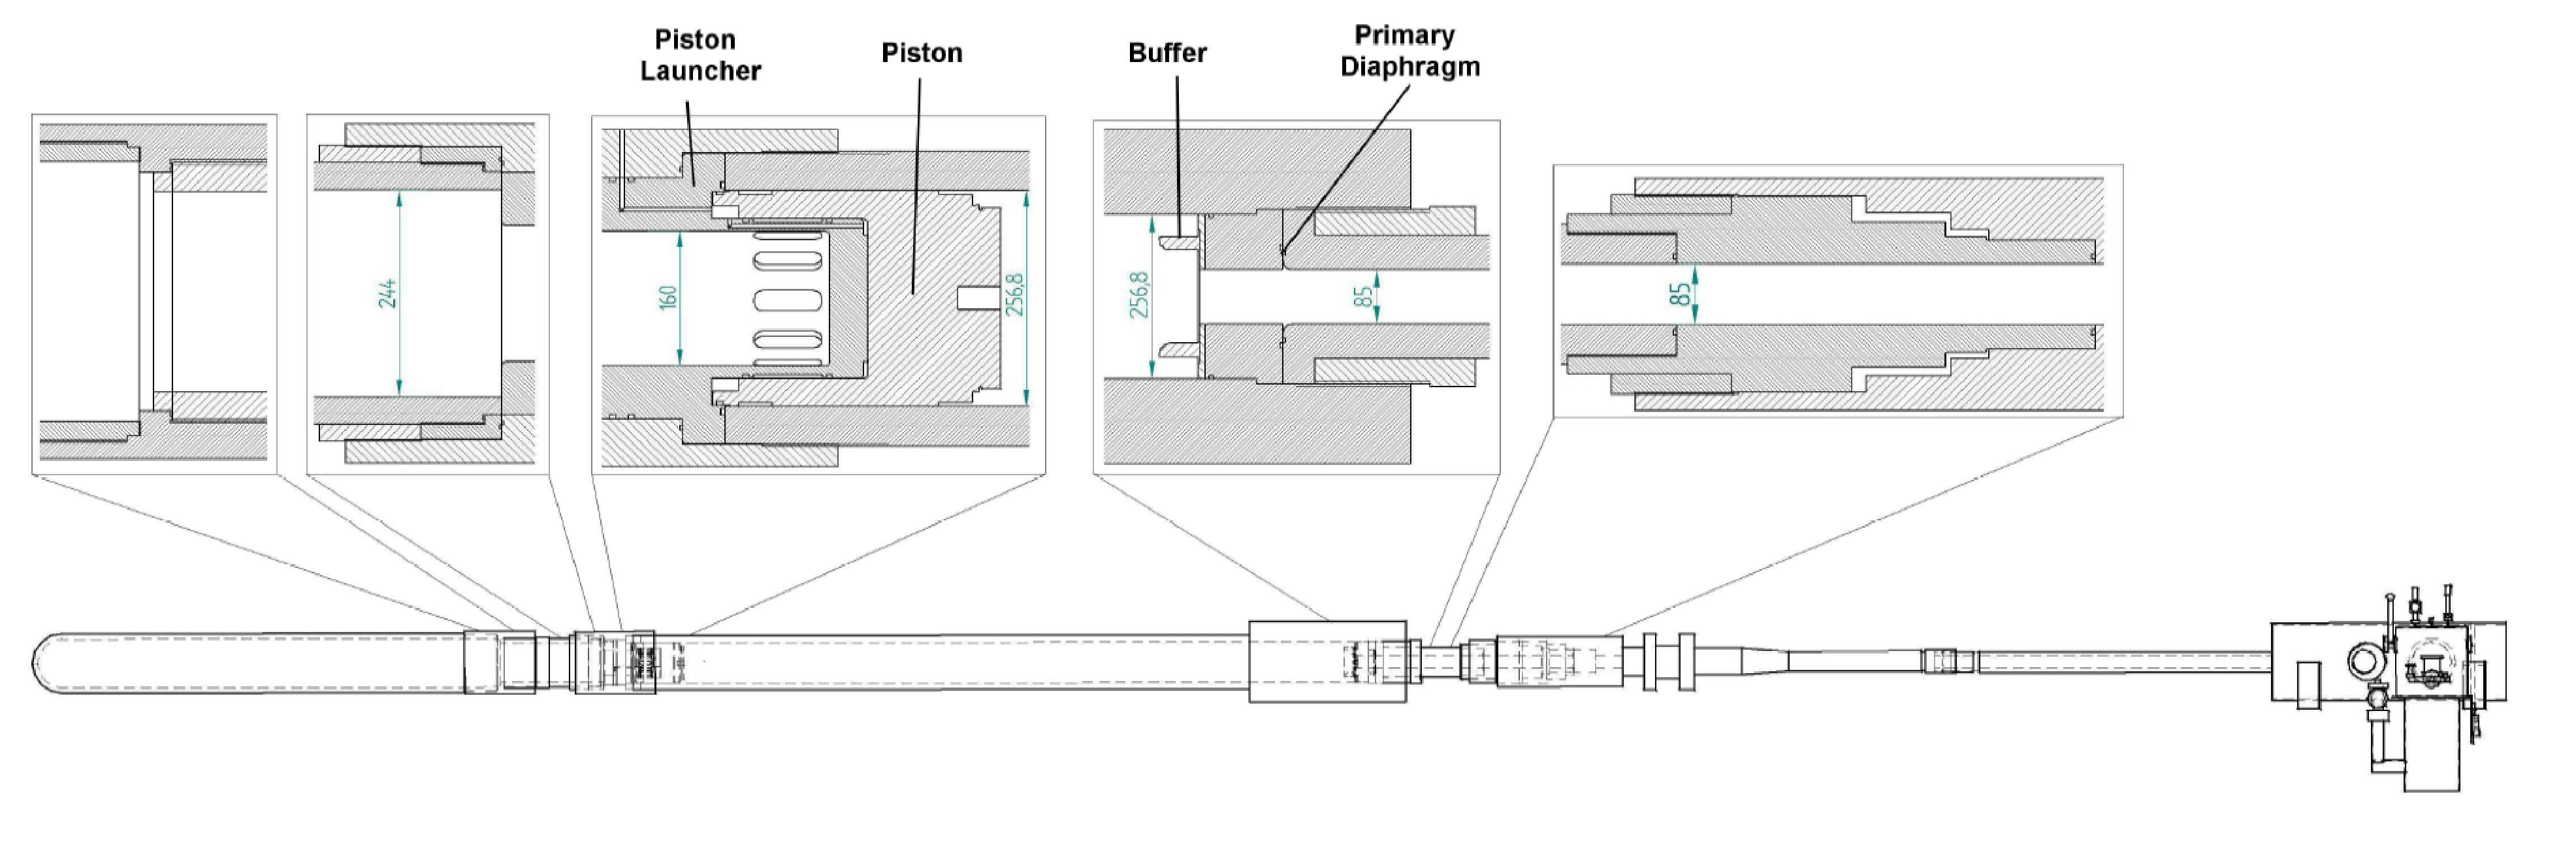
\includegraphics[scale=0.2]{figs/x2_plan.eps}
\caption{The X2 expansion tube with free-piston driver as of April 2005 \cite{reno2}}
\label{fig:x2_tube} 
\end{figure}

\par \medskip

Due to the low filling pressures required for expansion tube conditions, the lightest possible secondary diaphragm is used to reduce jetting of the driver gas at the interface and minimise freestream dissociation.  Typically `half-thou' mylar diaphragms with a burst pressure of 45kPa are used to separate the test and accelerator gas.  Even the lightest possible diaphragm materials have been shown to generate a substantial reflected shock upstream of the diaphragm at rupture \cite{bakos}, and for this reason the hold-time model is implemented in L1d when simulating these conditions.

\medskip

\begin{table}[htb]
\begin{center}  % put inside center environment
\begin{tabular*}{0.8\textwidth}%
     {@{\extracolsep{\fill}}cccc}
\hline \hline \textbf{Condition}                                     & \textbf{Air}    & \textbf{Mars} & \textbf{Jupiter} \\
\hline Patching window, $\Delta t_{RSP} (\mu s)$         & 0.7    &  0.8  & 0.4    \\
Shock-front cells, $n_{shock}$                           & 9      &   8   &  8     \\
Rarefaction cells, $n_{rare}$                            & 144    &  179  &  84    \\
Shock speed, $U_{s} (km_{s})$                            & 11.4   &  8.2  &  20.3  \\
Internal pressure, $p^{*} (kPa)$                         & 45     &  5    &  40.4  \\
Internal velocity, $u^{*} (m_{s})$                       & 9520   &  6800 &  16910 \\
Total pressure, $p_{total} (MPa)$                        & 2.6    &  0.4  &  1.4   \\
Total enthalpy, $H_{total} (MJ/kg)$                      &  57    &  47   &  239   \\
Global shift, $\Delta x_{global} (1.0 \times 10^{-6} m)$ &   6.6  &  3.2  &  10.8  \\
Shock shift, $\Delta x_{shock} (m)$                      &   0    &  0    &  0     \\
\hline
\end{tabular*}
\caption{Summary of RSP procedures performed in L1d for the three X2 expansion tube test cases}
\label{table:x2_rsp}
\end{center}
\end{table}

A summary of the RSP procedure for each of the X2 conditions investigated is shown in \emph{Table \ref{table:x2_rsp}}.  Higher density upstream slugs result in more cells being incorporated in the expansion wave than for the ideal shock tube.  The three conditions test the RSP modules ability to handle the full range of total enthalpies and pressures encountered in expansion tubes.  The severity of the Jupiter condition, however, reveals the RSP modules inability to account for viscous mass loss to the boundary layer.  Such a capability may be considered in a future study.

\subsubsection{9km/s Air Condition}

Michael Scott developed this condition for the evaluation of the modifications made to X2 in 2005, namely the free-piston single-stage driver and the Mach 9 hypersonic nozzle \cite{scott}.  \emph{Table \ref{table:x2_air_fills}} summarises the initial fill conditions and resulting shock speeds obtained from shot \emph{x2s18}.  This is a classic expansion tube condition in that it is conducted at both high total enthalpy ($H_{total} \approx 50MJ/kg$) and total pressure ($p_{total} \approx 2 MPa$), and is therefore a useful test case for the RSP module.

\par \medskip

A variety of $\Delta t_{RSP}$ values were trialled as to gauge the sensity of the solution to this parameter.  \emph{Figure \ref{fig:air_various_rsp_dts:a}} compares the pressure profiles $5 \mu s$ after diaphragm rupture for $\Delta t_{RSP}$ values ranging between 0.5 and 1.0 $\mu s$, and \emph{Figure \ref{fig:air_various_rsp_dts:b}} displays the detail in the temperature profile ahead of the interface. 

\begin{table}[hbc]
\begin{center}  % put inside center environment
\begin{tabular*}{0.65\textwidth}%
     {@{\extracolsep{\fill}}cc}
\hline Reservoir Fill (MPa of Air) & 1.8 \\
Driver Fill (mBar) & $480 \pm 1$ \\
Driver Gas & 100 \% Helium \\
Primary Diaphragm & 1.6mm steel \\
Secondary Diaphragm & 3-ply polyethylene \\
Shock tube (kPa test gas) & $ 10 \pm 0.1$ \\
Acceleration Tube (Pa air) & $35 \pm 0.5$ \\
\textbf{Shock Velocities (m/s)} \\
Shock Tube & $4800 \pm 100$ \\
Acc. Tube (end) & $9000 \pm 200$   \\
\hline
\end{tabular*}
\caption{Initial fill conditions and shock speeds for 9km/s air condition conducted in X2}
\label{table:x2_air_fills}
\end{center}
\end{table}

\begin{figure}[hb]
\centering
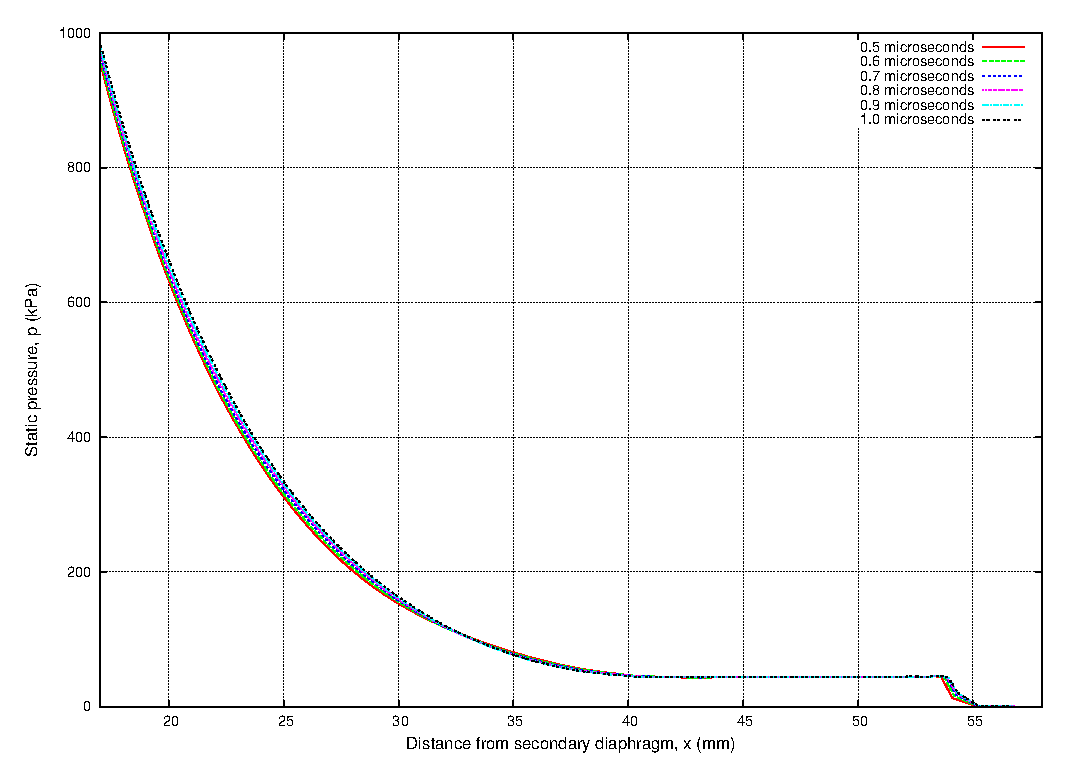
\includegraphics[scale=0.8]{figs/air_vrspdts_press_profile.eps}
\caption{Pressure profile through the front half of the wave-pattern at $5 \mu s$ after diaphragm rupture for the 9km/s air condition with various $\Delta t_{RSP}$ durations}
\label{fig:air_various_rsp_dts:a}
\end{figure}

\begin{figure}[hc]
\centering
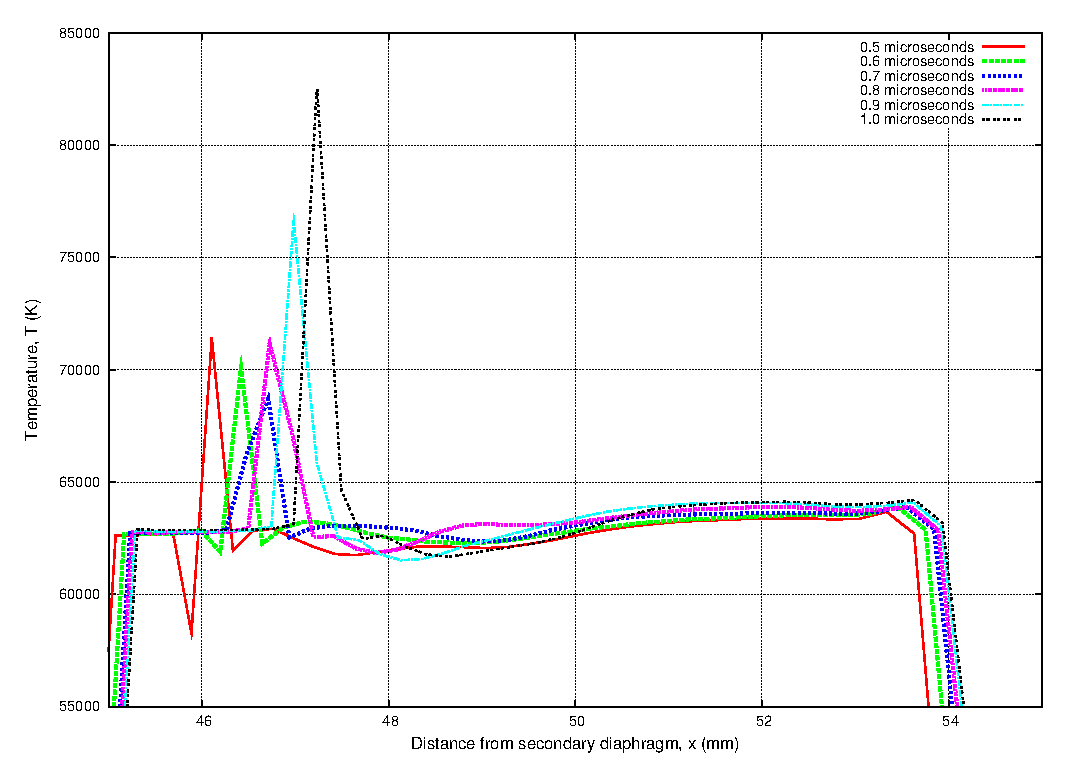
\includegraphics[scale=0.8]{figs/air_vrspdts_temp_profile_detail.eps}
\caption{Temperature profile detail ahead of the interface at $5 \mu s$ after diaphragm rupture for the 9km/s air condition with various $\Delta t_{RSP}$ durations}
\label{fig:air_various_rsp_dts:b}
\end{figure}

While the general form of the flow profiles appears to be insensitive to the patching window, the magnitude of the discontinuity just downstream of the contact surface varies appreciably.  The temperature discontinuity resulting from using the largest $\Delta t_{RSP}$ value of $1 \mu s$ is significant, and is seen to dissipate by reducing the patching window.  An optimal value of $\Delta t_{RSP}$ is reached at $0.7 \mu s$, whilst further reduction of the patching window results in a slightly larger discontuity.  This can be attributed to the low cell resolution of the shorter $\Delta t_{RSP}$, with the shock being only captured over two cells for the $0.5 \mu s$ case.

\par \medskip

\begin{figure}[hb]
\centering
\subfigure[Pressure profile] % caption for subfigure a
{
    \label{fig:air_iv_press_profile}
    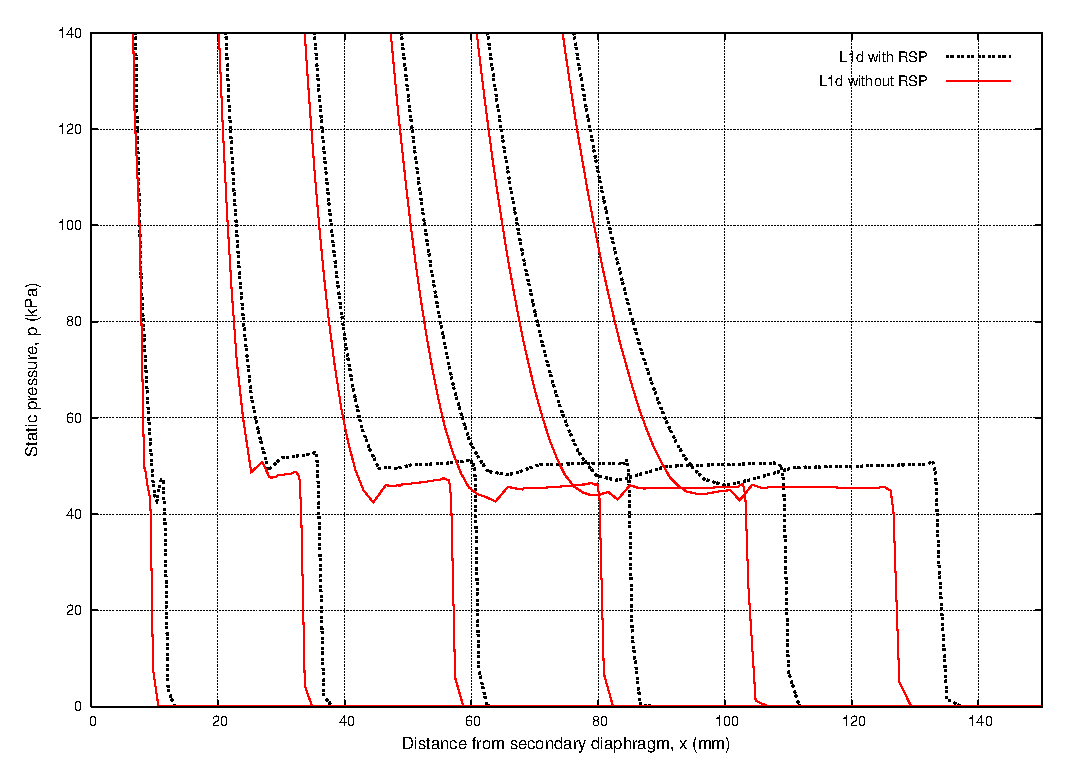
\includegraphics[scale=0.45]{figs/air_iv_press_profile.eps}
} \hspace{0cm}
\subfigure[Temperature profile detail] % caption for subfigure b
{
    \label{fig:air_iv_temp_profile}
    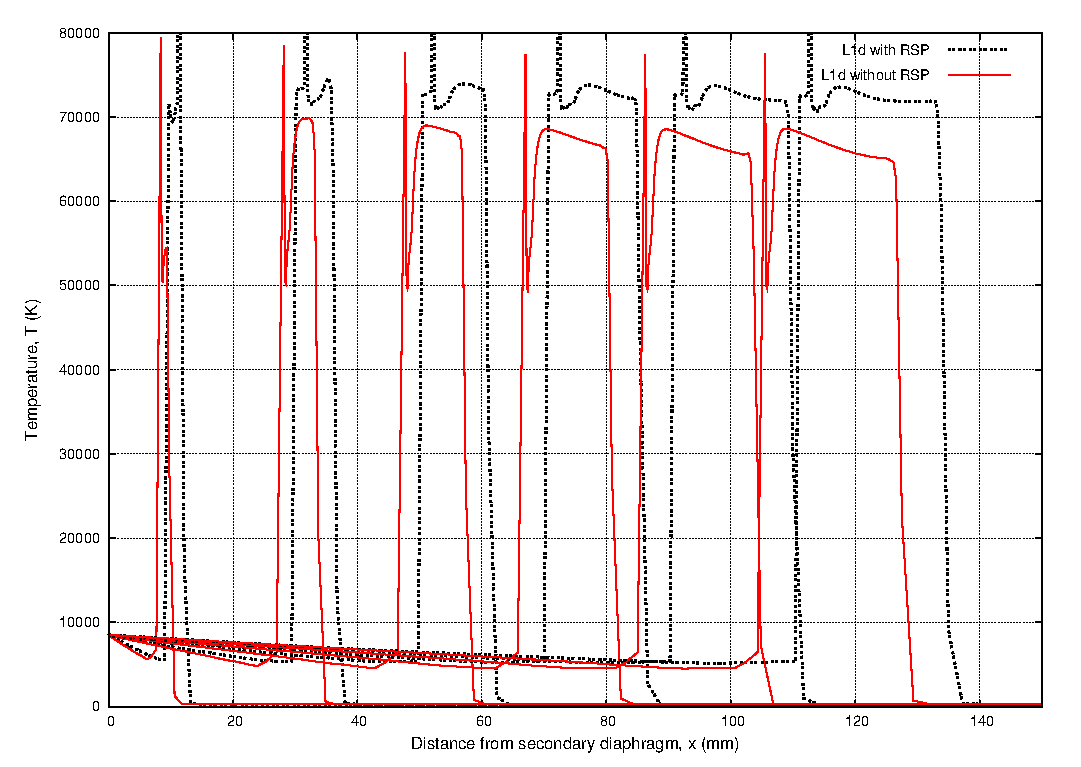
\includegraphics[scale=0.45]{figs/air_iv_temp_profile.eps}
} \caption{Inviscid L1d flow profiles for a 9km/s air condition in the X2 expansion tube with $t_{hold} = 10 \mu s$ and $\Delta t_{RSP} = 0.7 \mu $ (profiles for the first $10 \mu s$ after diaphragm rupture displayed)}
\label{fig:air_iv_profiles} % caption for the whole figure
\end{figure}

\emph{Figure \ref{fig:air_profiles_viscous}} displays the flow profiles for the first $10 \mu s$ following rupture for $\Delta t_{RSP} = 0.7 \mu s$.  The patched Riemann solution is initially described by 144 cells through the expansion wave and 9 cells in the shock front.  The description of the contact surface in the standard L1d solution is poor, with all the displayed profiles exhibiting strong discontuities either side of the interface.  Implementing the RSP module almost entirely elimates these features.  The stength of the resulting shock is increased slightly, with the shock speed travelling 5\% faster and a similar increase in the shock front flow properties.  The shock is quickly attenuated as it travels down the acceleration tube to match that of the standard solution \footnote{The two shock speeds are the same when using a temporal resolution of 1 $\mu s$ for the flow history between each transducer location}.  A noticable dip in the fully expanded test gas pressure also emerges in the patched solution.

\par \medskip

An inviscid comparision was also conducted to assess the influence of viscosity during the initial development of the wave-pattern.  \emph{Figure \ref{fig:air_iv_profiles}} compares the pressure and temperature profiles from the standard and patched L1d solutions for the inviscid simulations (see \emph{Appendix \ref{appendix_B}} for the complete set of inviscid flow profiles).  The shock from the patched solution is still slightly stronger, and a substanital increase in the shocked accelerator gas pressure occurs after the Riemann solution has been patched into L1d.  It is interesting to note that the drop in the fully expanded test gas pressure observed in the inviscid patched solution also occurs in both the inviscid simulations; the viscous RSP and inviscid standard solutions are in fact very similar.  This indicates viscous effects during the initial wave-pattern development are substantial in L1d, and the RSP module suffers from neglecting its influence on the flow.

\par \medskip

These discrepencies, however, do not persist as the flow travels down the acceleration tube.  \emph{Figure \ref{fig:air_atx}} compares the static pressure history at final two transducer locations as the shock reaches the end of the acceleration tube for the standard the patched viscous L1d solutions.  Experimentally obtained pressure traces from shots \emph{x2s18} and \emph{x2s19} are overlayed for reference.  The structure of the L1d pressure trace is not changed durastically, with a slight drop in pressure occuring at the head of the expansion wave.  Although the shock is seen to arrive earlier at both transducer locations for the patched solution, the average shock speed between all transducers along the tube remains unchanged.  The difference in arrival time is attributed to the gradual development of the shock front in the first few microseconds following rupture for the standard solution.

\begin{figure}[htb]
  \begin{center}
    \mbox{
      \subfigure[Pressure]
      {
         \label{fig:sub:k}
         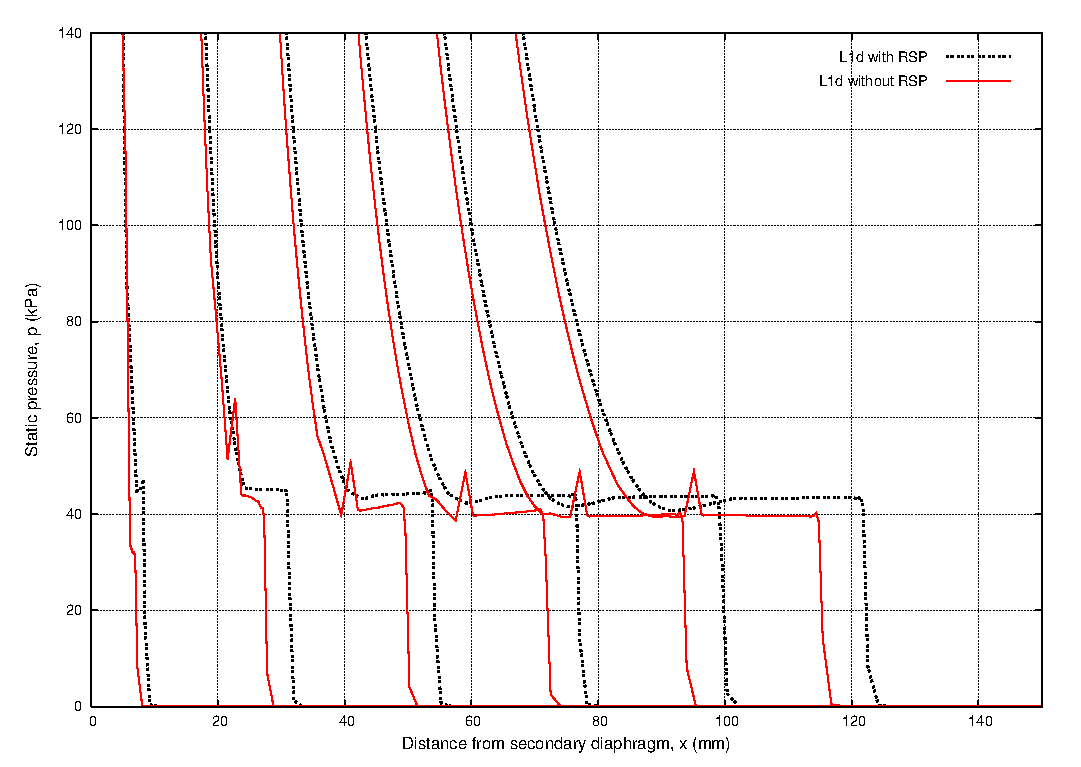
\includegraphics[scale=0.45]{figs/air_press_profile.eps}
      } \quad
      \subfigure[Temperature]
      {
         \label{fig:sub:l}
         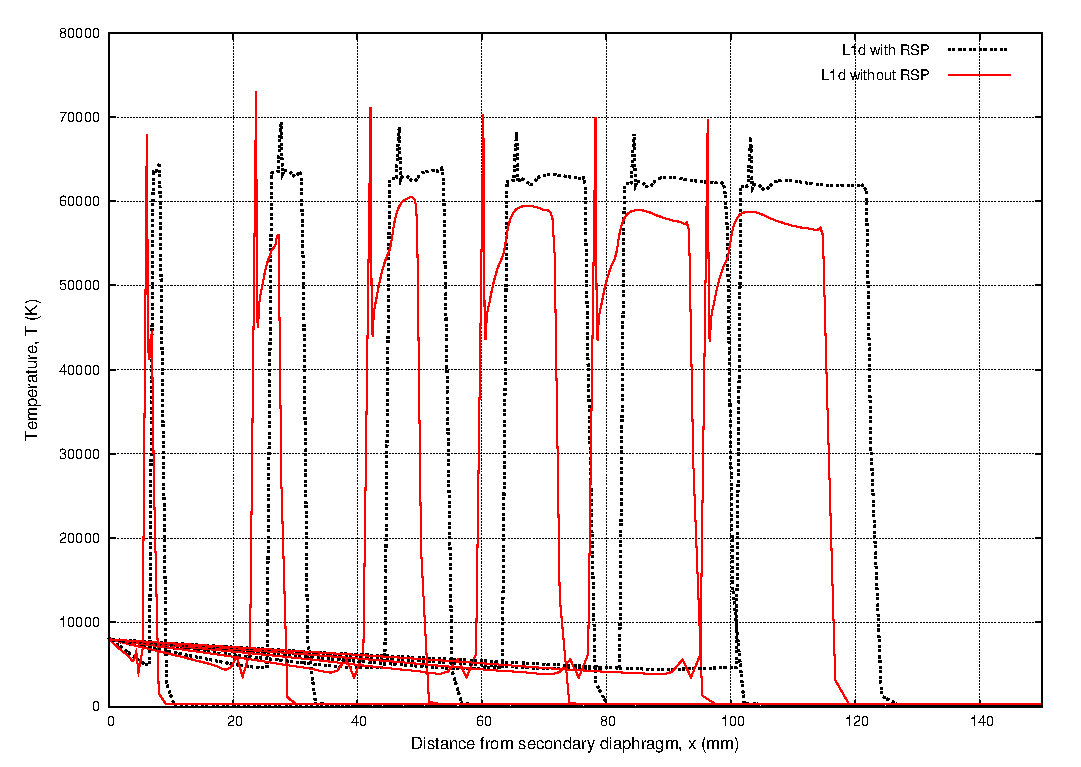
\includegraphics[scale=0.45]{figs/air_temp_profile.eps}
      }
      }
    \mbox{
      \subfigure[Density]
      {
         \label{fig:sub:m}
         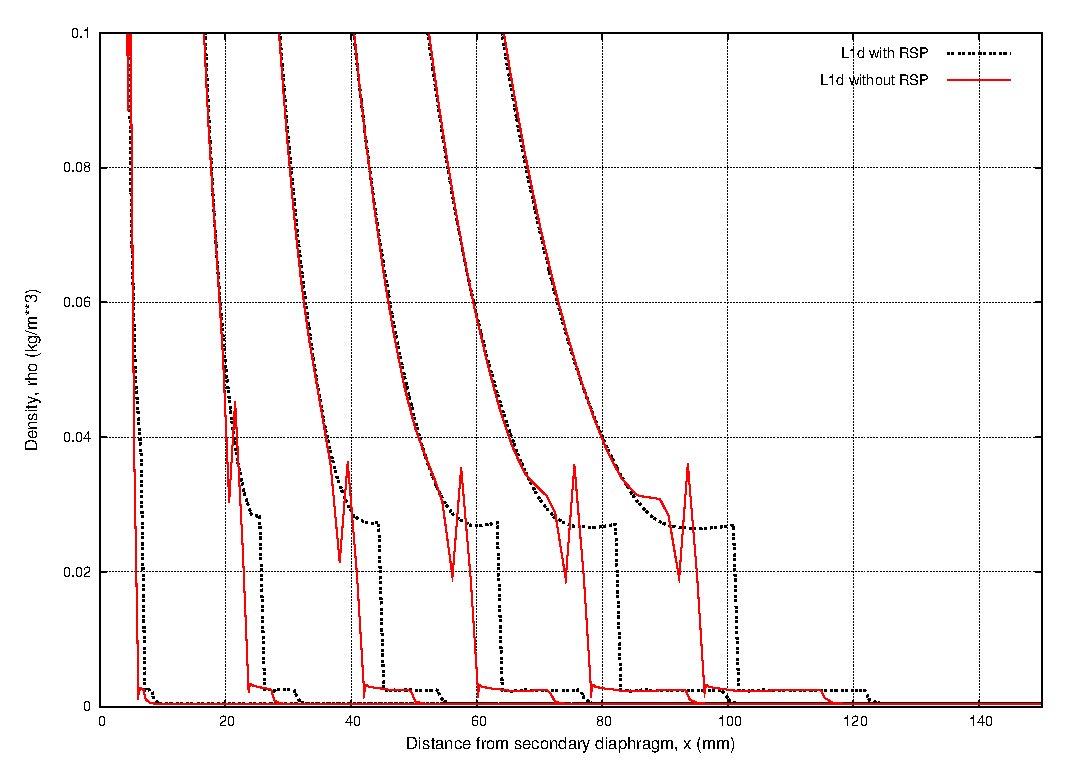
\includegraphics[scale=0.45]{figs/air_density_profile.eps}
      } \quad
      \subfigure[Velocity]
      {
         \label{fig:sub:n}
         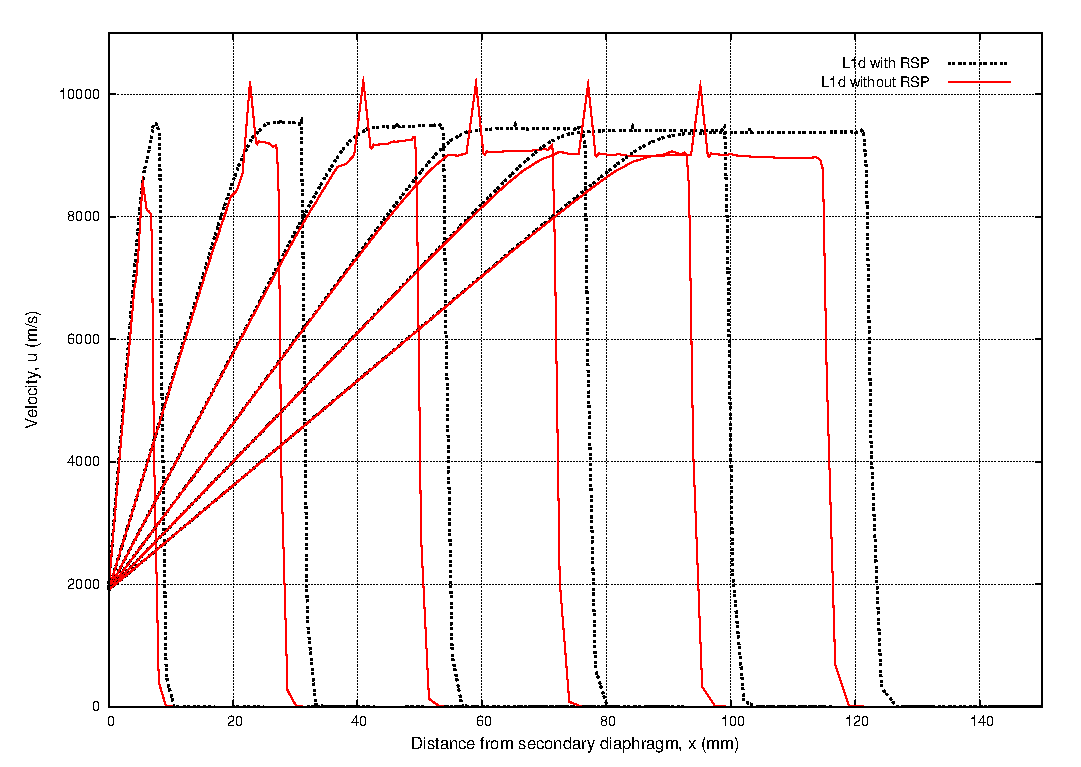
\includegraphics[scale=0.45]{figs/air_velocity_profile.eps}
      } 
      }
    \caption{Viscous L1d flow profiles for a 9km/s air condition in the X2 expansion tube with $t_{hold} = 10 \mu s$ and $\Delta t_{RSP} = 0.7 \mu $ (flow profiles for the first $10 \mu s$ after diaphragm rupture displayed)}
    \label{fig:air_profiles_viscous}
  \end{center}
\end{figure}

\begin{figure}[p]
\centering
\subfigure[AT4] % caption for subfigure a
{
    \label{fig:air_at4}
    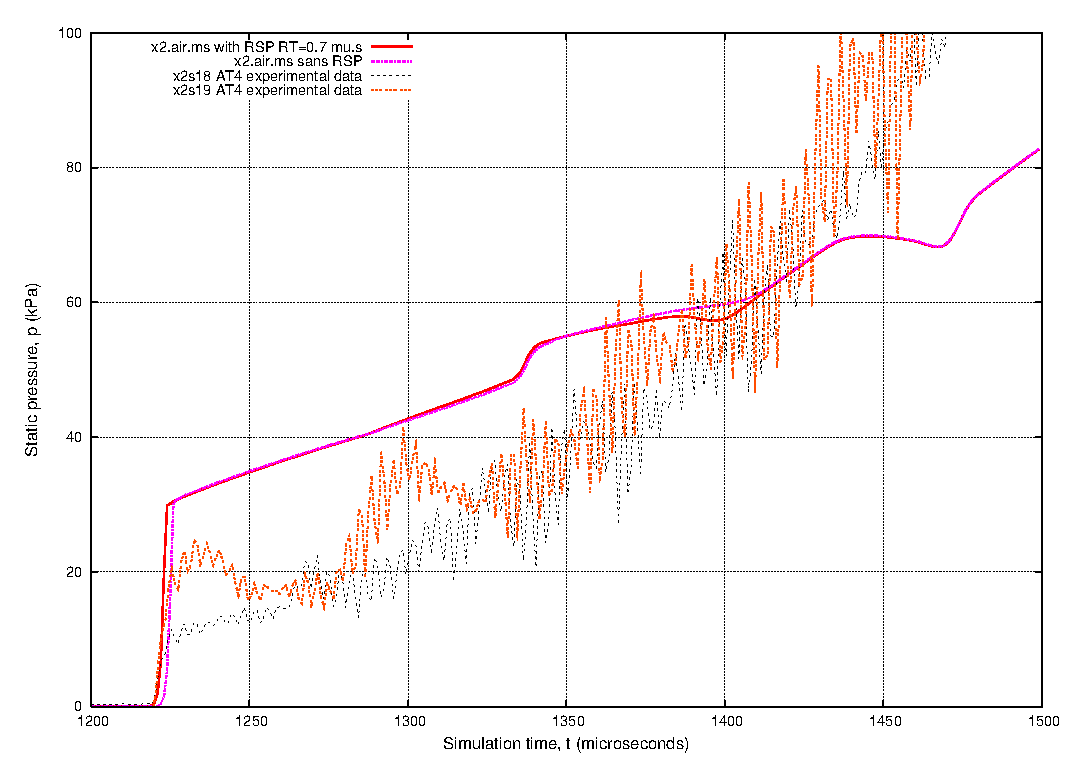
\includegraphics[scale=0.8]{figs/air_at4_press.eps}
} \hspace{0cm}
\subfigure[AT5] % caption for subfigure b
{
    \label{fig:air_at5}
    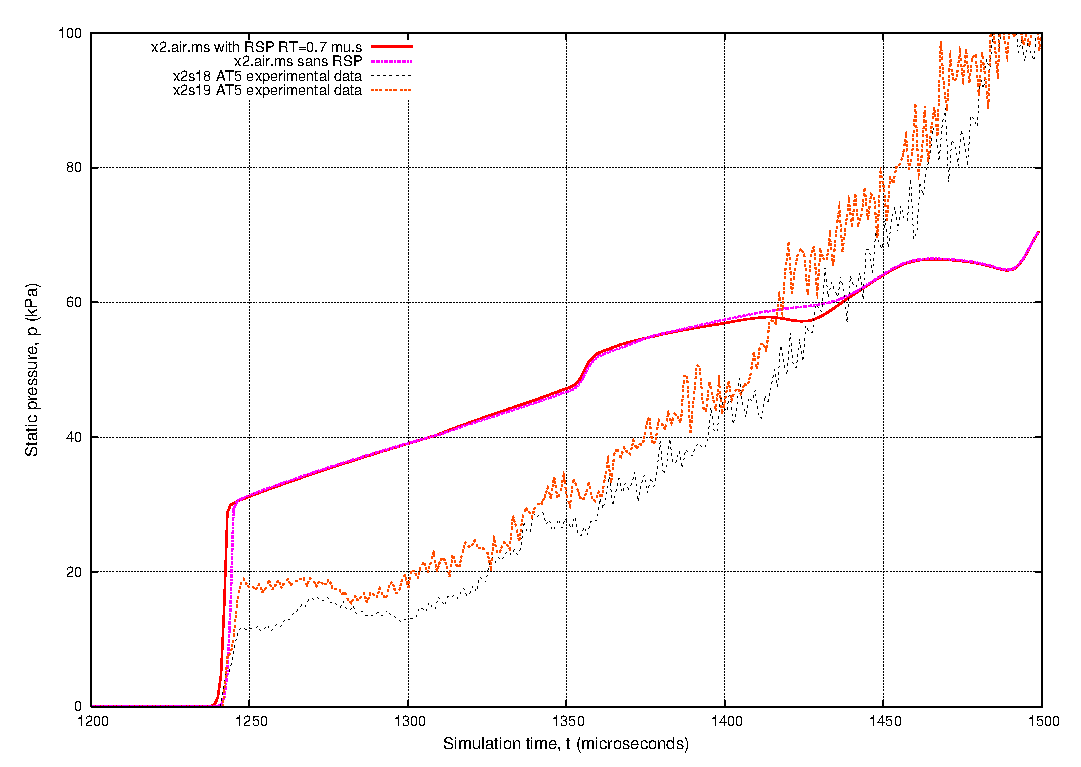
\includegraphics[scale=0.8]{figs/air_at5_press.eps}
} \caption{Static pressure histories at various acceleration tube transducer locations for the 9km/s air condition in the X2 expansion tube}
\label{fig:air_atx} % caption for the whole figure
\end{figure}


\subsubsection{6.6km/s Mars Condition}

The 6.6km/s Mars Condition was designed to evaluate the ability of X2 to produce conditions suitable for the subscale testing of highspeed aerocapture conditions through the Martian atmosphere.  A soft-driver condition is used that is designed to minimise the severity of the piston impact with the buffer following the compression stroke.  \emph{Table \ref{table:x2_mars_fills}} summarises the initial fill conditions and resulting shock speeds obtained from shot \emph{x2s173}.  This condition is of significantly lower total enthalpy and pressure compared to the 9km/s air condition, with $E_{total} \approx 40 MJ/kg$ and $p_{total} \approx 60kPa$.

\begin{table}[hb]
\begin{center}  % put inside center environment
\begin{tabular*}{0.65\textwidth}%
     {@{\extracolsep{\fill}}cc}
\hline Reservoir Fill (MPa of Air) & 1.25 \\
Driver Fill (mBar) & $300 \pm 1$ \\
Driver Gas & 83\% Ar 17\% He \\
Primary Diaphragm & 1.0mm steel \\
Secondary Diaphragm & 1/2 thou mylar \\
Shock tube (Pa test gas) & $3500 \pm 50$ \\
Acceleration Tube (Pa air) & $9 \pm 0.5$ \\
\textbf{Shock Velocities (m/s)} \\
Shock Tube & $3300 \pm 100$ \\
Acc. Tube (end) & $6550 \pm 150$   \\
\hline
\end{tabular*}
\caption{Initial fill conditions and shock speeds for 6.6km/s Mars condition conducted in X2}
\label{table:x2_mars_fills}
\end{center}
\end{table}

\begin{figure}[htb]
  \begin{center}
    \mbox{
      \subfigure[Pressure]
      {
         \label{fig:sub:o}
         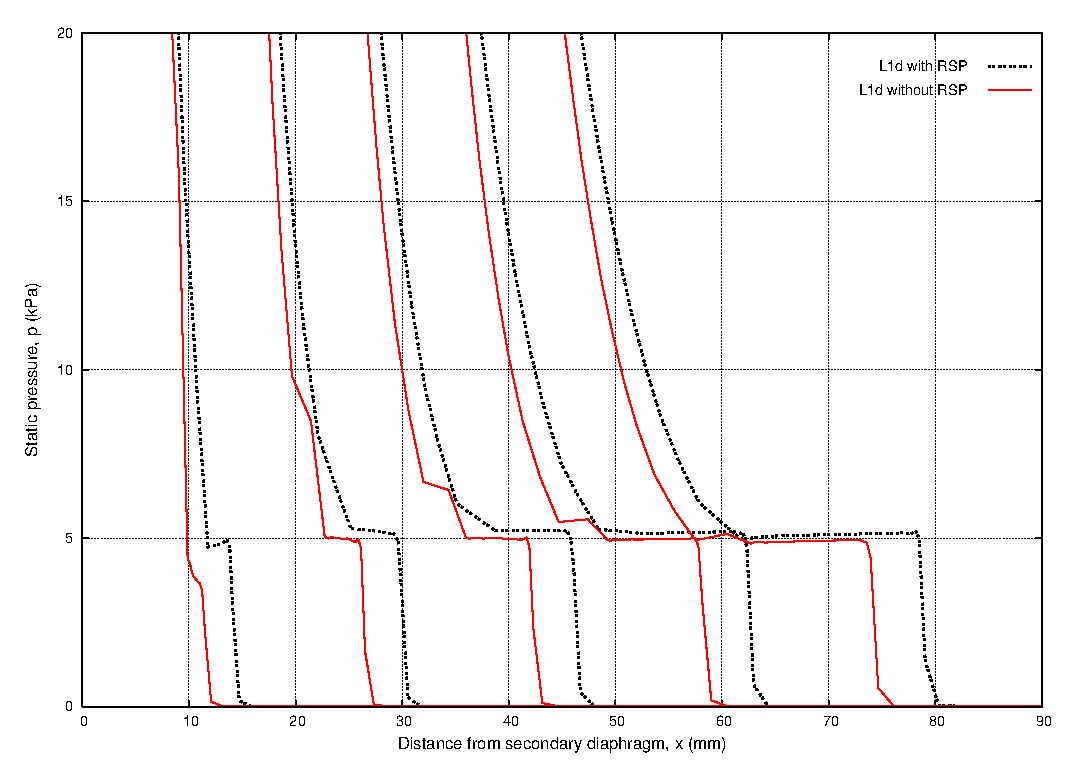
\includegraphics[scale=0.43]{figs/mars_press_profile.eps}
      } \quad
      \subfigure[Temperature]
      {
         \label{fig:sub:p}
         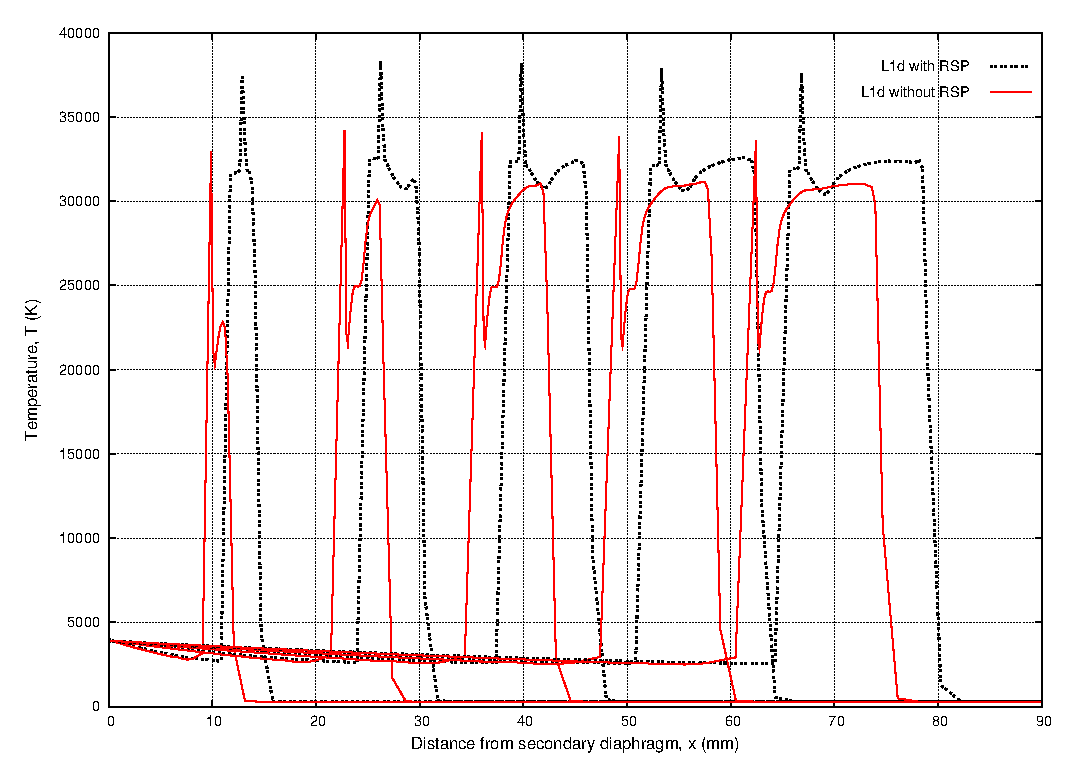
\includegraphics[scale=0.43]{figs/mars_temp_profile.eps}
      }
      }
    \mbox{
      \subfigure[Density]
      {
         \label{fig:sub:q}
         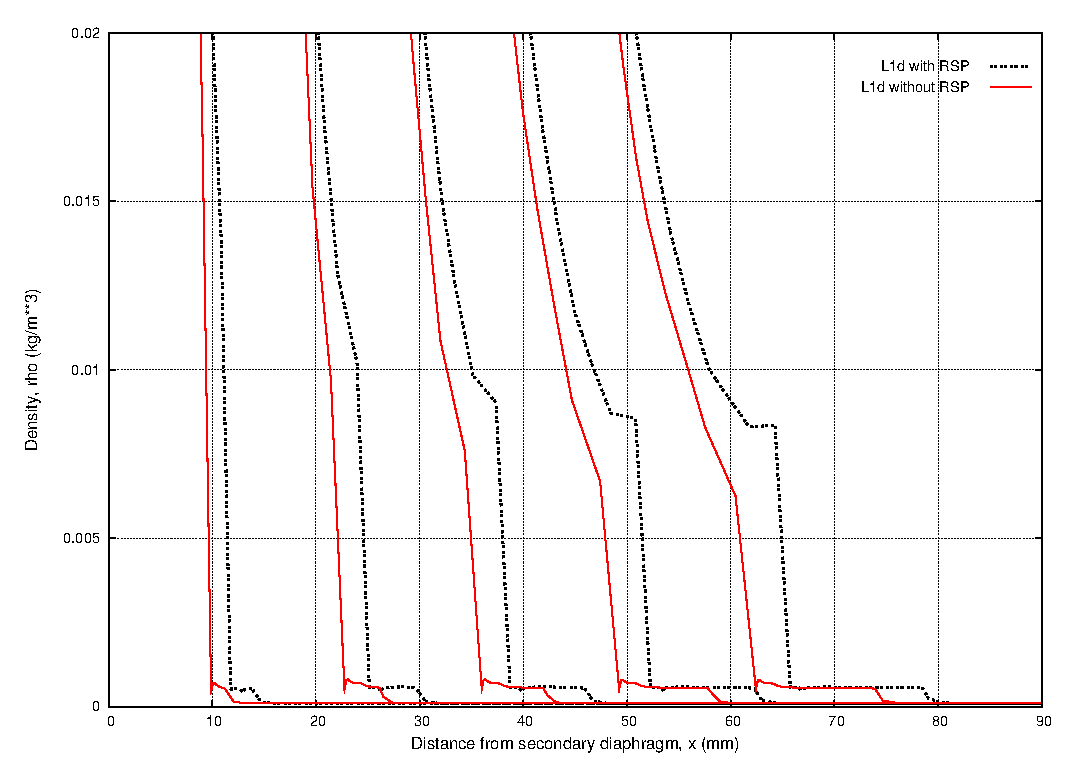
\includegraphics[scale=0.43]{figs/mars_density_profile.eps}
      } \quad
      \subfigure[Velocity]
      {
         \label{fig:sub:r}
         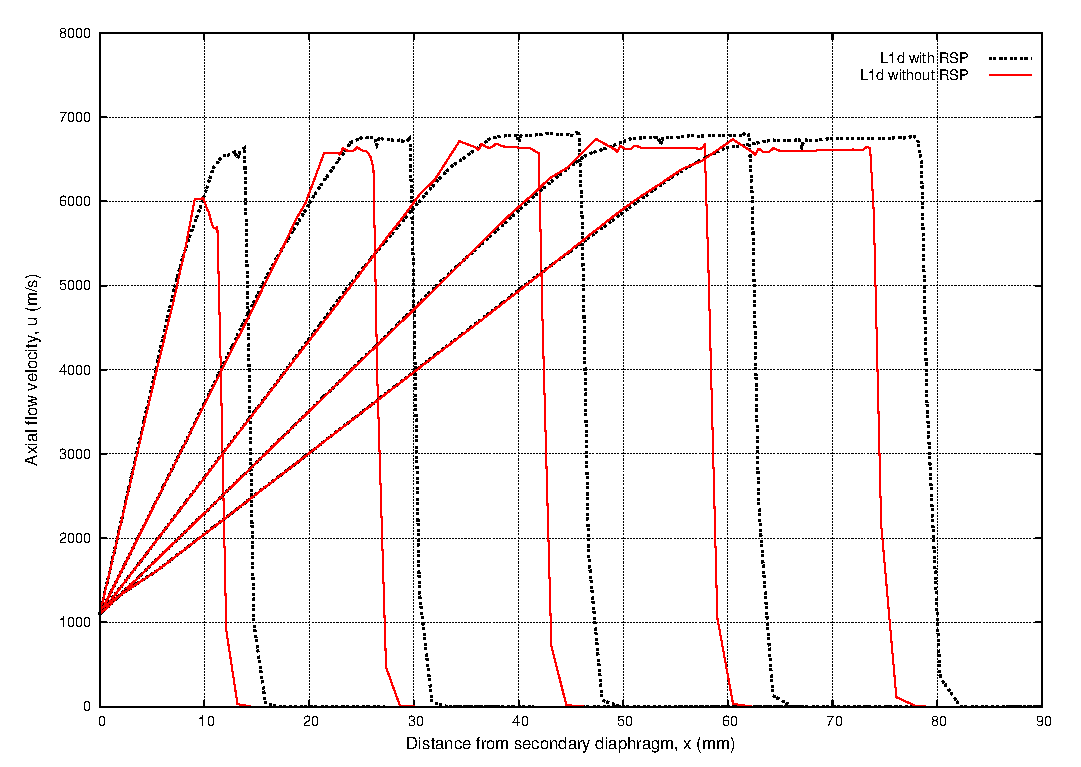
\includegraphics[scale=0.43]{figs/mars_velocity_profile.eps}
      } 
      }
    \caption{Viscous flow profiles for a 6.6km/s Mars gas condition in the X2 expansion tube}
    \label{fig:mars_profiles_viscous}
  \end{center}
\end{figure}

\emph{Figure \ref{fig:mars_profiles_viscous}} compares the flow profiles for the first $10 \mu s$ following rupture for $\Delta t_{RSP} = 0.8 \mu s$.   Good agreement is shown for the internal flow states either side of the contact surface, with a maximum 5\% variation existing in the shocked temperature.  Although the shock in the patched solution leads that from the standard solution by an everage of $4mm$, only a slight difference in shock speed exists at the end of the first $10\mu s$.  The shock gradually builds up to its fully developed strength in the standard solution, whereas the Riemann solution is ideal and is assumed to evolve steadily.  The standard L1d handles this condition reasonably well, with the exception of the poorly resolved fully expanded test gas and usual discontinuities ahead of the contact surface.  The patched solution allows the steady flow region to be captured more accurately, and reduces the property variation through the shock front. A similar comparision can be made for the inviscid flow profiles displayed in \emph{Appendix \label{appendix_B}}

\medskip

The static pressure history at transducer locations mid-length and near the end of the acceleration tube for the standard the patched viscous L1d solutions are shown in \emph{Figure \ref{fig:mars_atx}}, with experimental pressure traces overlayed for reference.  A similiar drop in pressure at the rarefaction head as for the air condition is observed at both transducer locations.  The experimental traces, most notably AT5 of shot \emph{x2s177}, also exhibit a plateau in pressure at a similar point in the flow, although the similarity is not definitive.  The RSP solution does not adversely affect the agreement with experimental data, and may even slightly improve it for this condition.

\begin{figure}p]
\centering
\subfigure[AT3] % caption for subfigure a
{
    \label{fig:mars_at3}
    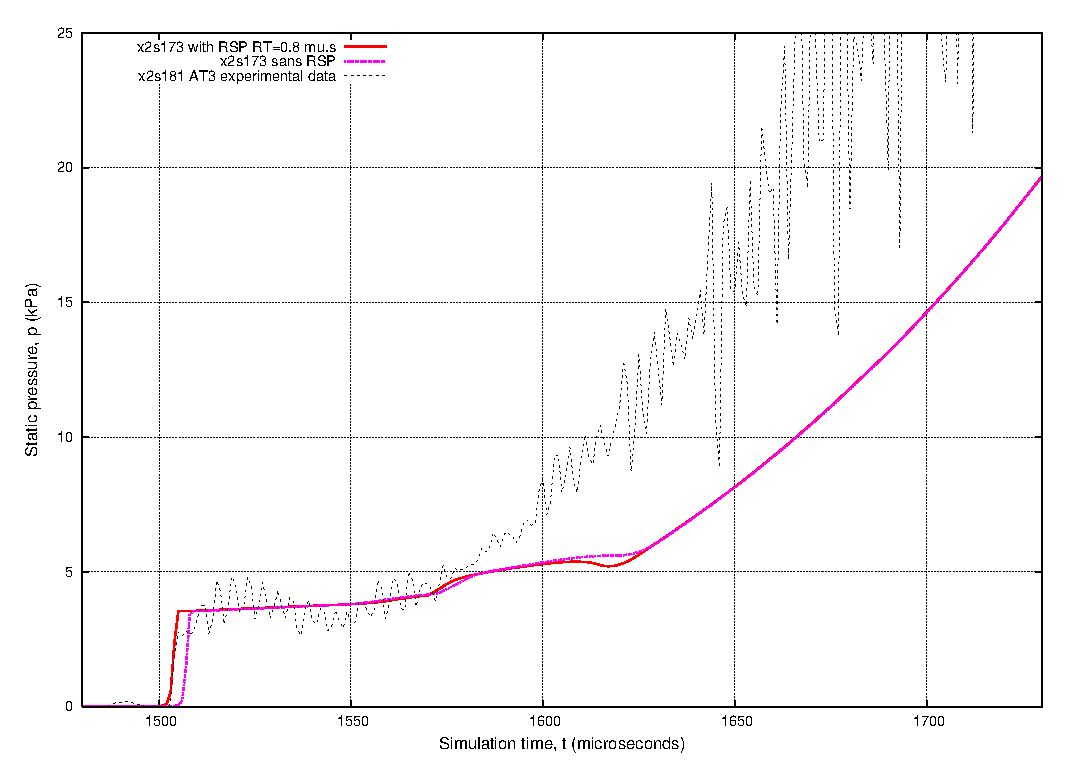
\includegraphics[scale=0.8]{figs/mars_at3_press.eps}
} \hspace{0cm}
\subfigure[AT5] % caption for subfigure b
{
    \label{fig:mars_at5}
    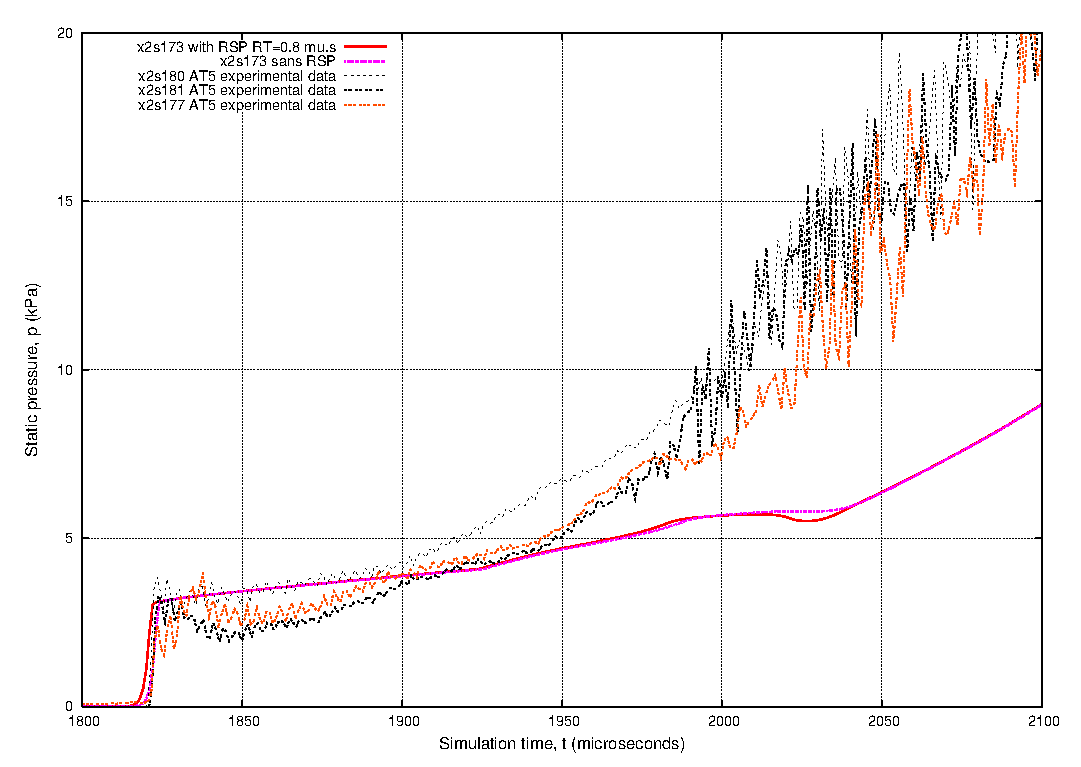
\includegraphics[scale=0.8]{figs/mars_at5_press.eps}
} \caption{Static pressure histories at various acceleration tube transducer locations for the 6.6km/s Mars condition in the X2 expansion tube}
\label{fig:mars_atx} % caption for the whole figure
\end{figure}

\subsubsection{11km/s Jupiter Condition}

\begin{table}[h]
\begin{center}  % put inside center environment
\begin{tabular*}{0.65\textwidth}%
     {@{\extracolsep{\fill}}cc}
\hline Reservoir Fill (MPa of Air) & 1.8 \\
Driver Fill (mBar) & $480 \pm 1$ \\
Driver Gas & 100 \% Helium \\
Primary Diaphragm & 1.6mm steel \\
Secondary Diaphragm & 1-ply polyethylene \\
Shock tube (kPa test gas) & $ 3 \pm 0.1$ \\
Acceleration Tube (Pa air) & $ 10 \pm 0.5$ \\
\textbf{Shock Velocities (m/s)} \\
Shock Tube & $5500 \pm 100$ \\
Acc. Tube (end) & $10400 \pm 200$   \\
\hline
\end{tabular*}
\caption{Initial fill conditions and shock speeds for 11km/s Jupiter condition conducted in X2}
\label{table:x2_jupiter_fills}
\end{center}
\end{table}

This condition was designed for studying hydrogen dissociation and ionisation during entry into Jupiter's atmosphere at superorbital speeds.  Whilst Jupiter's atmosphere consists largely of hydrogen with a small percentage of helium, the test gas used for this condition is $15\%$ $H_{2}$ and $85\%$ Ne.  Substituting the small helium fraction with a larger proportion of an inert diluent, such as Neon, allows the binary chemical kinetic processes that lead to hydrogen dissociation and ionisation to be reproduced at achievable flow speeds \cite{edwards}.  \emph{Table \ref{table:x2_jupiter_fills}} summarises the fill conditions and L1d input parameters for this simulation.  The original driver configuration bursting a 1.6mm steel diaphragm at 25MPa was used for this condition, as was for the 9km/s air condition.

\par \medskip

The inability of L1d to handle the secondary diaphragm rupture for this condition was the primary motivation for the development of the RSP module \cite{my_ug_thesis}.  Unfortunately it is for this specific condition that the inadequacies of the module are most obvious. The initial flow profiles following rupture are shown in 
\emph{Figure \ref{fig:jupiter_profiles}}.  The lack of viscous effects in the Riemann solution leads to the mass of the shock-front being considerably over predicted. The viscous interaction with the tube wall predicted in L1d in the first few timesteps is very high, resulting in substantial mass loss to the boundary layer.  While the initial pressure in the shock front predicted by L1d is actually the same as that from the Riemann solution, the extent of the shock front, and thus the incorporated mass, is much lower due.  As the shock develops, a new equilibrium interface pressure is attained as the small amount of higher pressure shocked gas expands infront of the weakening unsteady expansion wave.  These effects are ignored in the patched solution, and the resulting wave-pattern is considerably stronger.

\par \medskip

\begin{figure}[htbp]
  \begin{center}
    \mbox{
      \subfigure[Pressure]
      {
         \label{fig:sub:jpp}
         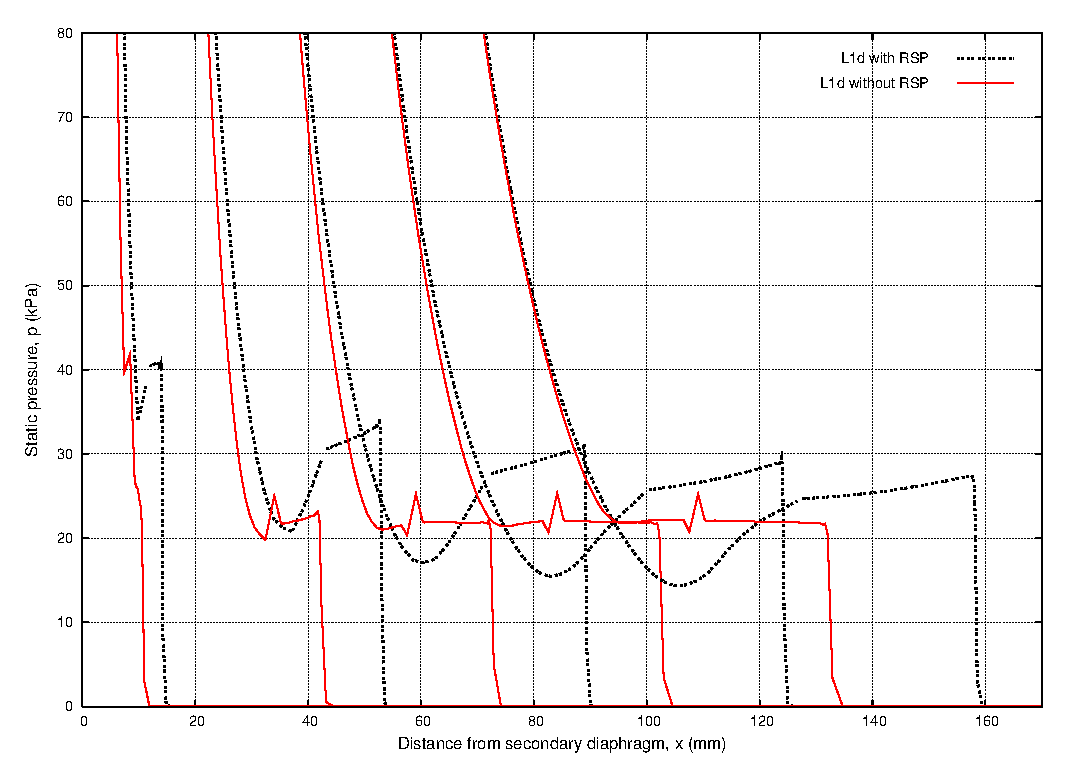
\includegraphics[scale=0.45]{figs/jupiter_press_profile.eps}
      } \quad
      \subfigure[Temperature]
      {
         \label{fig:sub:l}
         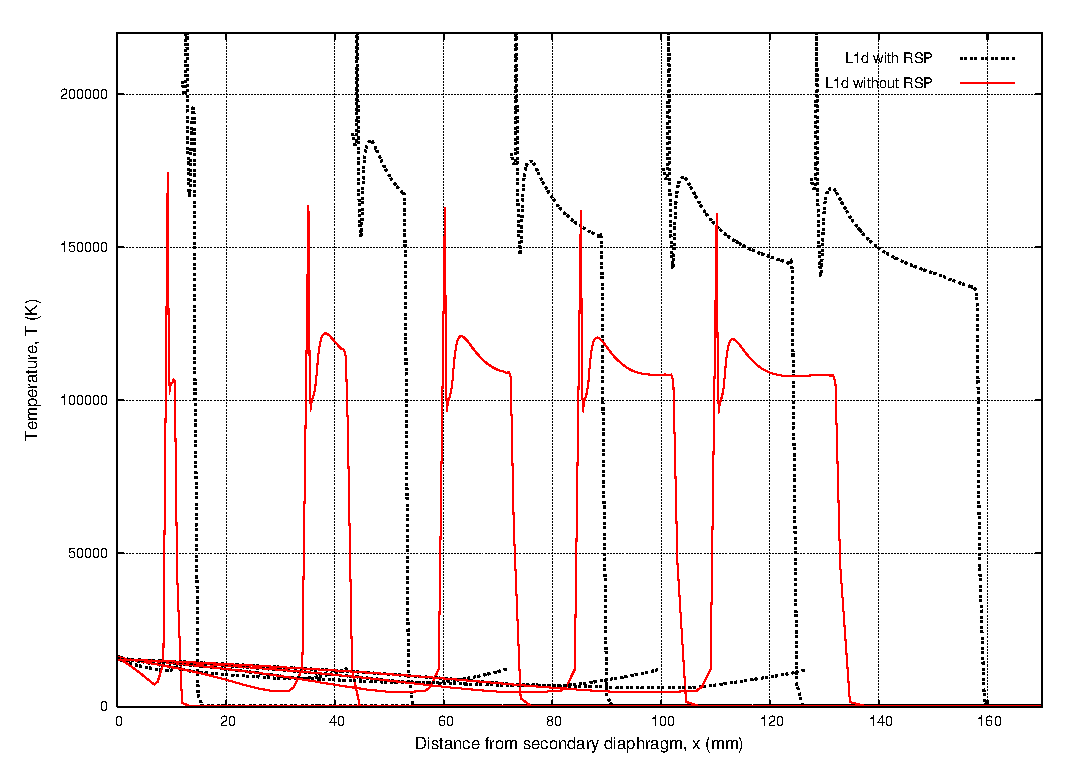
\includegraphics[scale=0.45]{figs/jupiter_temp_profile.eps}
      }
      }
    \mbox{
      \subfigure[Density]
      {
         \label{fig:sub:m}
         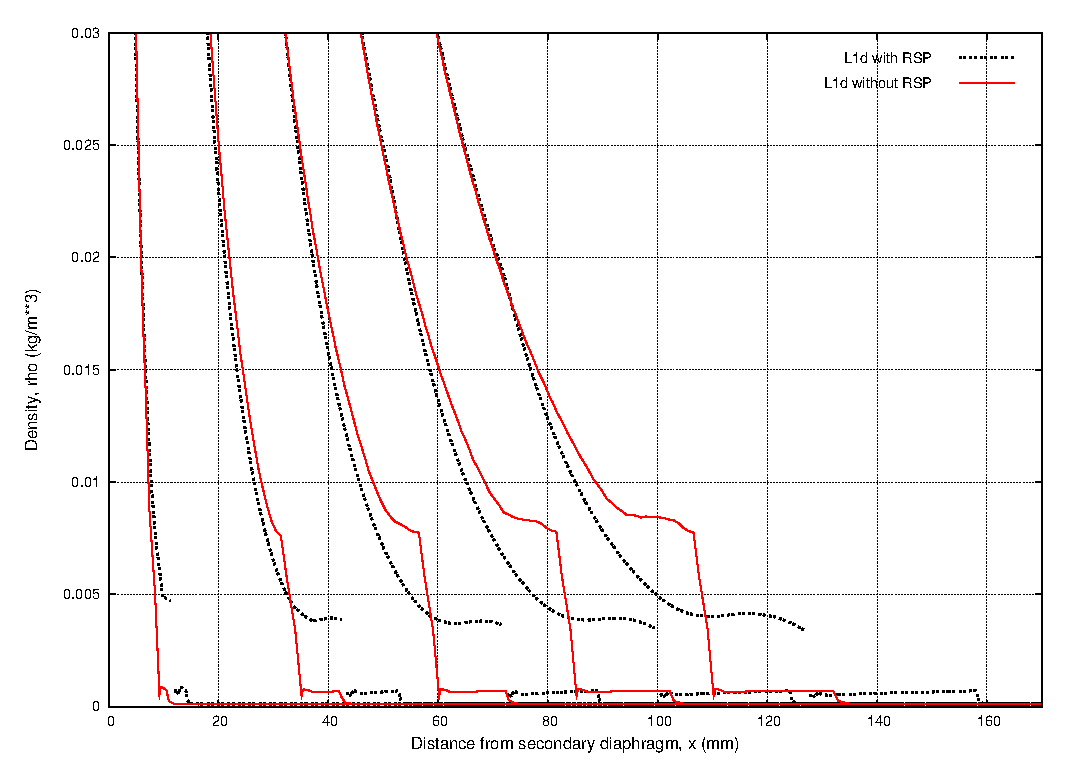
\includegraphics[scale=0.45]{figs/jupiter_dens_profile.eps}
      } \quad
      \subfigure[Velocity]
      {
         \label{fig:sub:n}
         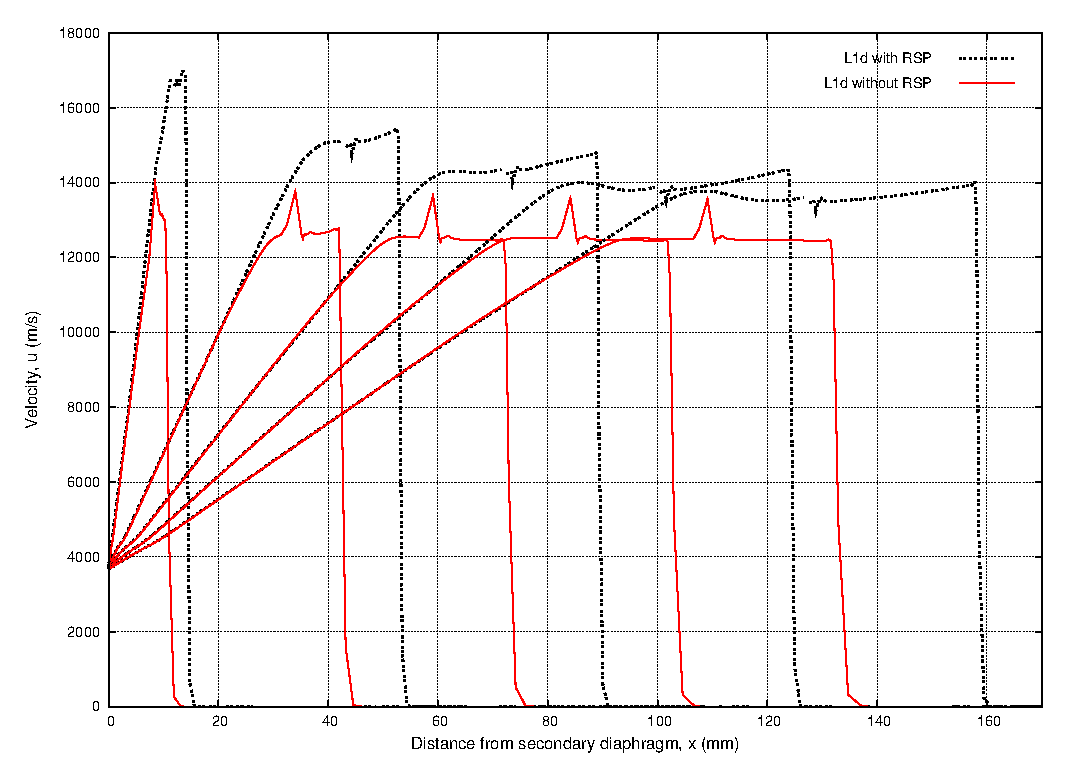
\includegraphics[scale=0.45]{figs/jupiter_velocity_profile.eps}
      } 
      }
    \caption{Viscous L1d flow profiles for a 11km/s Jupiter condition in the X2 expansion tube with $t_{hold} = 10 \mu s$ and $\Delta t_{RSP} = 0.4 \mu $ (flow profiles for the first $10 \mu s$ after diaphragm rupture displayed)}
    \label{fig:jupiter_profiles}
  \end{center}
\end{figure}

\begin{figure}[htbp]
  \begin{center}
    \mbox{
      \subfigure[AT2]
      {
         \label{fig:sub:m}
         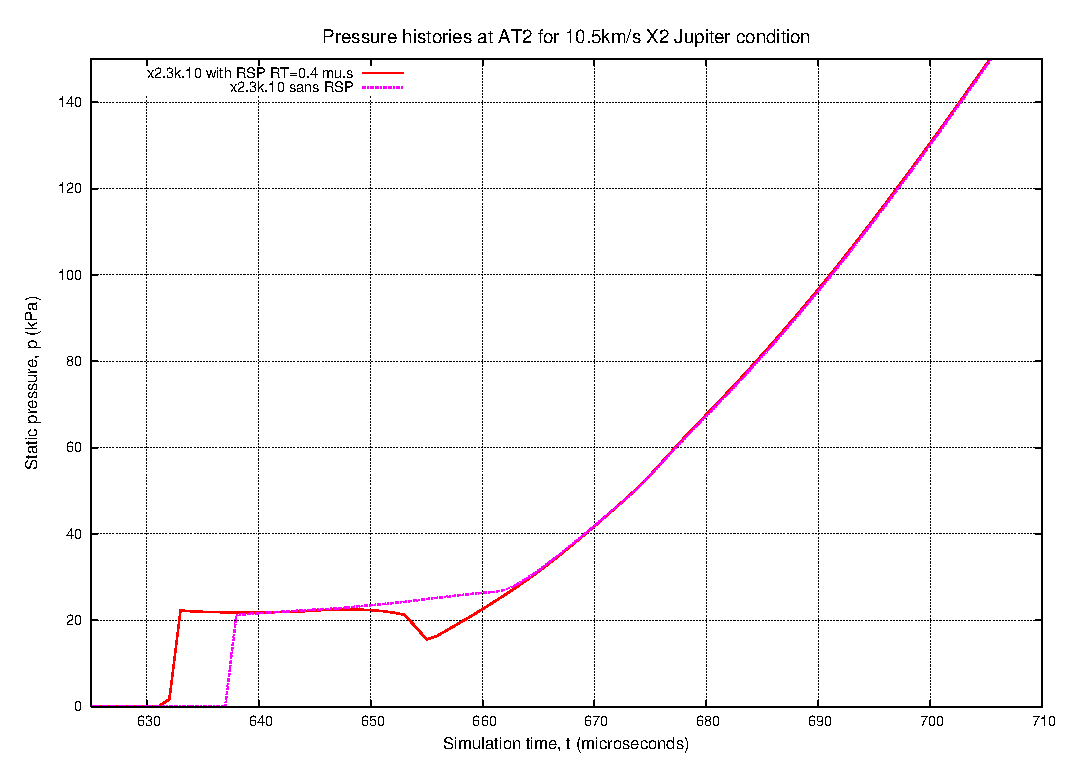
\includegraphics[scale=0.4]{figs/jupiter_at2_press.eps}
      } \quad
      \subfigure[AT3]
      {
         \label{fig:sub:n}
         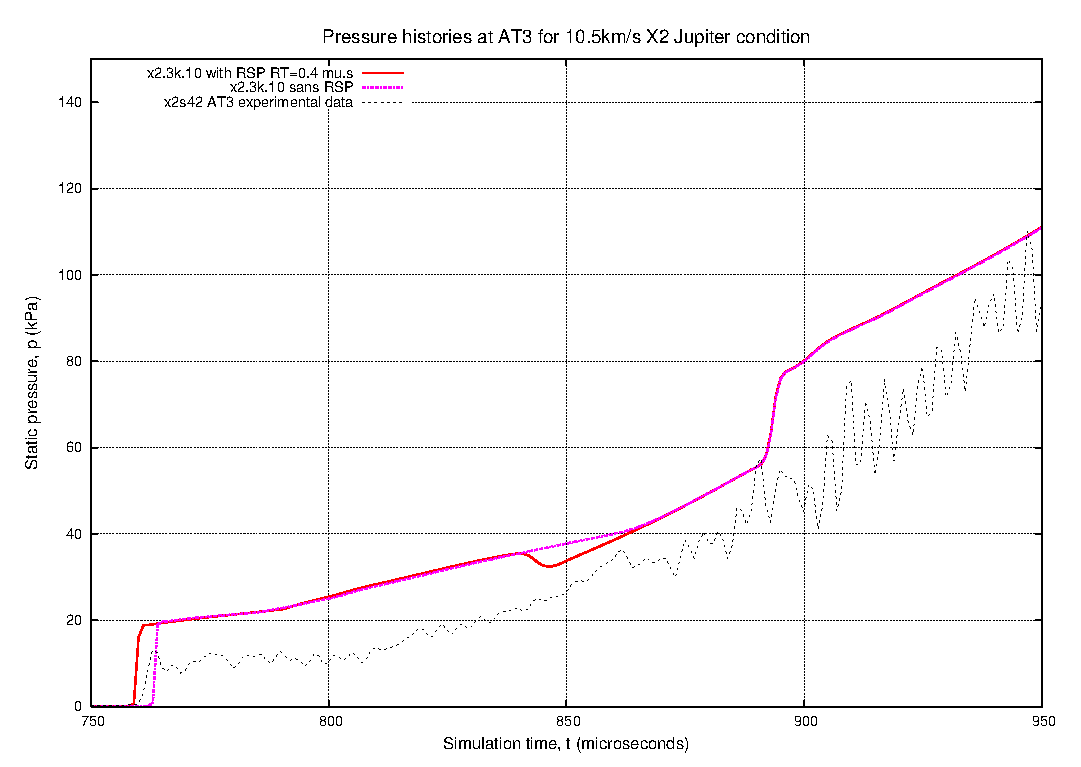
\includegraphics[scale=0.4]{figs/jupiter_at3_press.eps}
      }
      }
    \mbox{
      \subfigure[AT4]
      {
         \label{fig:sub:o}
         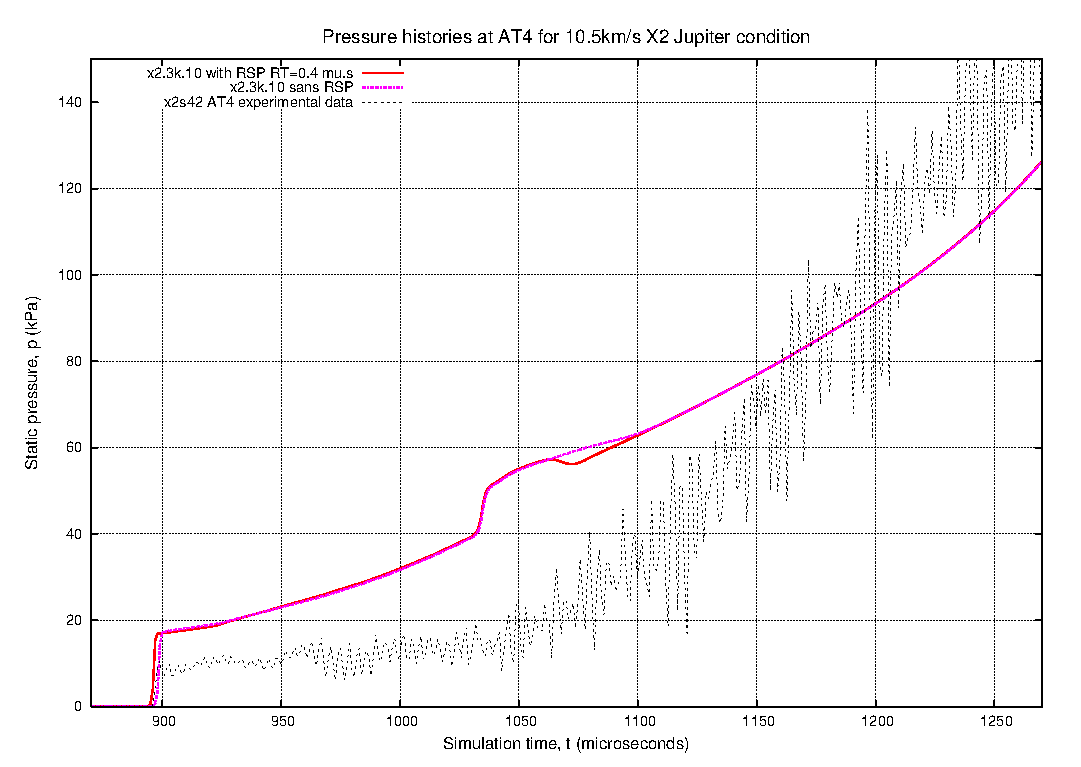
\includegraphics[scale=0.4]{figs/jupiter_at4_press.eps}
      } \quad
      \subfigure[AT5]
      {
         \label{fig:sub:p}
         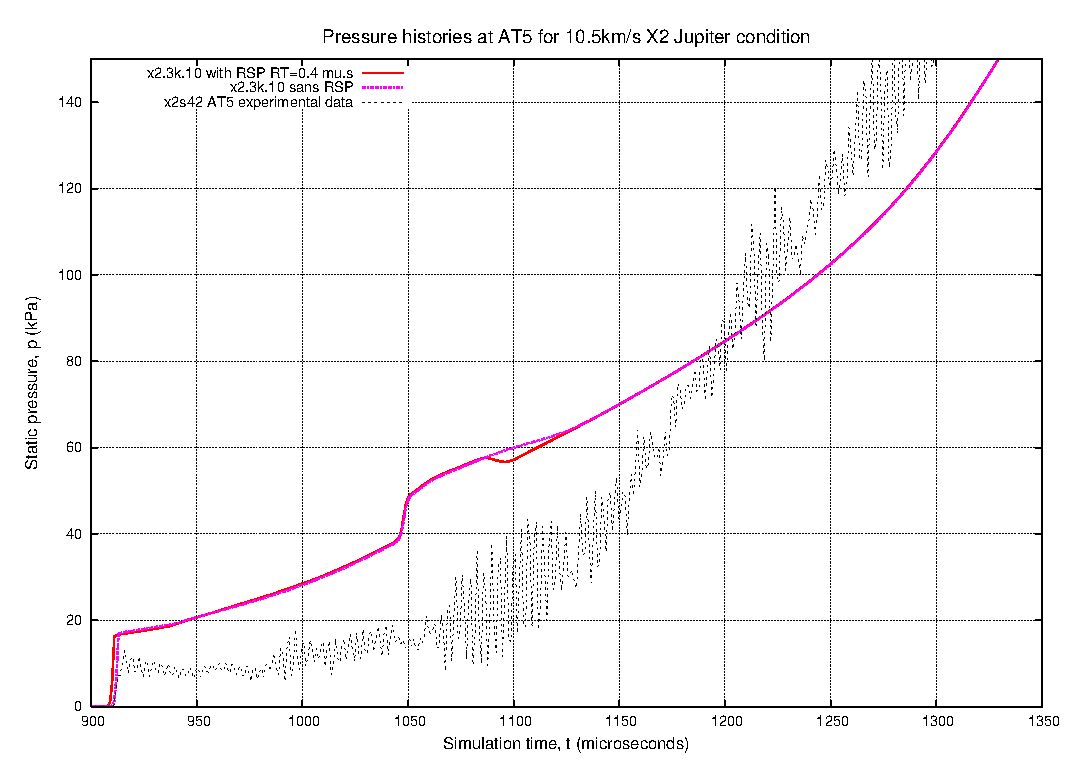
\includegraphics[scale=0.4]{figs/jupiter_at5_press.eps}
      } 
      }
    \caption{Static pressure histories at various acceleration tube transducer locations for the 11km/s Jupiter condition in the X2 expansion tube}
    \label{fig:jupiter_atx_p}
  \end{center}
\end{figure}

The variation between the solutions is short-lived, however, and the static pressure tracesalong the acceleration tube are similiar, \emph{Figure \ref{fig:jupiter_atx_p}}.  As was observed in the previous X2 test cases, there is a noticable drop in pressure at the head of the expansion wave, and the shock arrives earlier but at the same speed.  The patched solution has essentially pushed this mass towards the interface and enlarged the shock front.  Although both L1d solutions only vaguely resemble the experimentally obtained traces, the patched solution provides a slightly improved description.

\newpage

\newpage

\section{Concluding remarks}

Due to the low pressures encountered in expansion tube conditions, the Lagrangian L1d solutions generally will not always resolve the finer details of the flow development.  L1d is nonetheless a convenient engineering tool for designing expansion tube conditions and obtaining initial estimates for the freestream properties.  The RSP module has been demonstrated to dramatically improve the desciption of the contact surface and shock front for two ideal shock tube conditions, and applied with varying degrees of success to real expansion tube conditions from the X2 facility.  The Riemann solutions assumption of inviscid flow was identified as a mechanism for generating substantially stronger shocks than predicted by a standard L1d solution, however the effect over the entire length of the acceleration tube is negligible.  The conditions at the tube exit are not adversely affected, and in some cases slightly improved agreement with experimental static pressure traces was evident.  For high-enthalpy conditions, however, the magnitude of the temperature discontinuity in the shock front can become larger than in the standard solution.  The RSP module should therefore be used cautiously for conditions where viscous effects and very high temperatures are known to occur. 
\newpage

% Bibliography
\nocite{*}
\bibliographystyle{unsrt}
\bibliography{rsp}

\newpage

\appendix

\section{L1d flux calculations}
\label{appendix_A}

Of particular interest to the investigation at hand is the calculation of the flux terms for a given cell at time $t_{i+1}$ given the flow state at $t_{i}$.  A brief summary of the relevant governing equations as described by Jacobs \cite{jacobs_98b} thus follows.
\par
\medskip
The two flux terms calculated for each cell at every time step are that of momentum, \emph{Eq. \ref{l1d_momentum}}, and energy, \emph{Eq. \ref{l1d_energy}} through \emph{\ref{l1d_energy3}}.  Note that an overline represents a cell averaged value.  The rate of change of momentum is effectively a force balance on each cell, where $F_{wall}$ and $F_{loss}$ are forces applied to the fluid due to the presence of the containing walls and various fittings:

\begin{equation}
\frac{d}{dt} m_{j} \overline{u}_{j} = \left [ P_{j-\frac{1}{2}} A_{j-\frac{1}{2}} - P_{j+\frac{1}{2}} A_{j+\frac{1}{2}} + \overline{P}_{j} ( A_{j+1/2} - A_{j-1/2})- \overline{F_{wall}} - \overline{F_{loss}} \right ] \label{l1d_momentum}
\end{equation}

The rate of change of total energy in a given cell is expressed in terms of the work done at the left and right cell interfaces:

\begin{equation}
\frac{d}{dt} m_{j} \overline{E}_{j} = \left [ P_{j-\frac{1}{2}} A_{j-\frac{1}{2}} u_{j-\frac{1}{2}} - P_{j+\frac{1}{2}} A_{j+\frac{1}{2}} u_{j+\frac{1}{2}} + \overline{q}_{j} \right] \label{l1d_energy}
\end{equation}

where

\begin{equation}
\overline{q_{j}} = h \pi \overline{D} ( x_{j+1/2} - x_{j-1/2} ) ( T_{w} - T_{aw} ) \label{l1d_energy2}
\end{equation}

\begin{equation}
E = e+ \frac{1}{2}u^{2} \label{l1d_energy3}
\end{equation}


The term $\overline{q}_{j}$ is the rate of heat transfer into the cell.  The velocity terms at the cell interface boundaries are calculated using a two stage Riemann solver, where the intermediate flow state is first estimated by assuming isentropic wave interaction between two perfect gases, then corrected if a strong shock is deemed to exist.
\par
\medskip
Consider the scenario where a large unbalanced pressure and velocity suddenly exists across a cell interface, for example on the left, such that:
\par
\begin{equation}
P_{j-\frac{1}{2}} A_{j-\frac{1}{2}} u_{j-\frac{1}{2}} >> P_{j+\frac{1}{2}} A_{j+\frac{1}{2}} u_{j+\frac{1}{2}} + \overline{q}_{j} \label{inequality1}
\end{equation}
and
\begin{equation}
\frac{d}{dt} m_{j} \overline{E}_{j} >> 0. \label{inequality2}
\end{equation}

\begin{figure}[hbt]
\centering
\centerline{\resizebox{0.8\linewidth}{!}{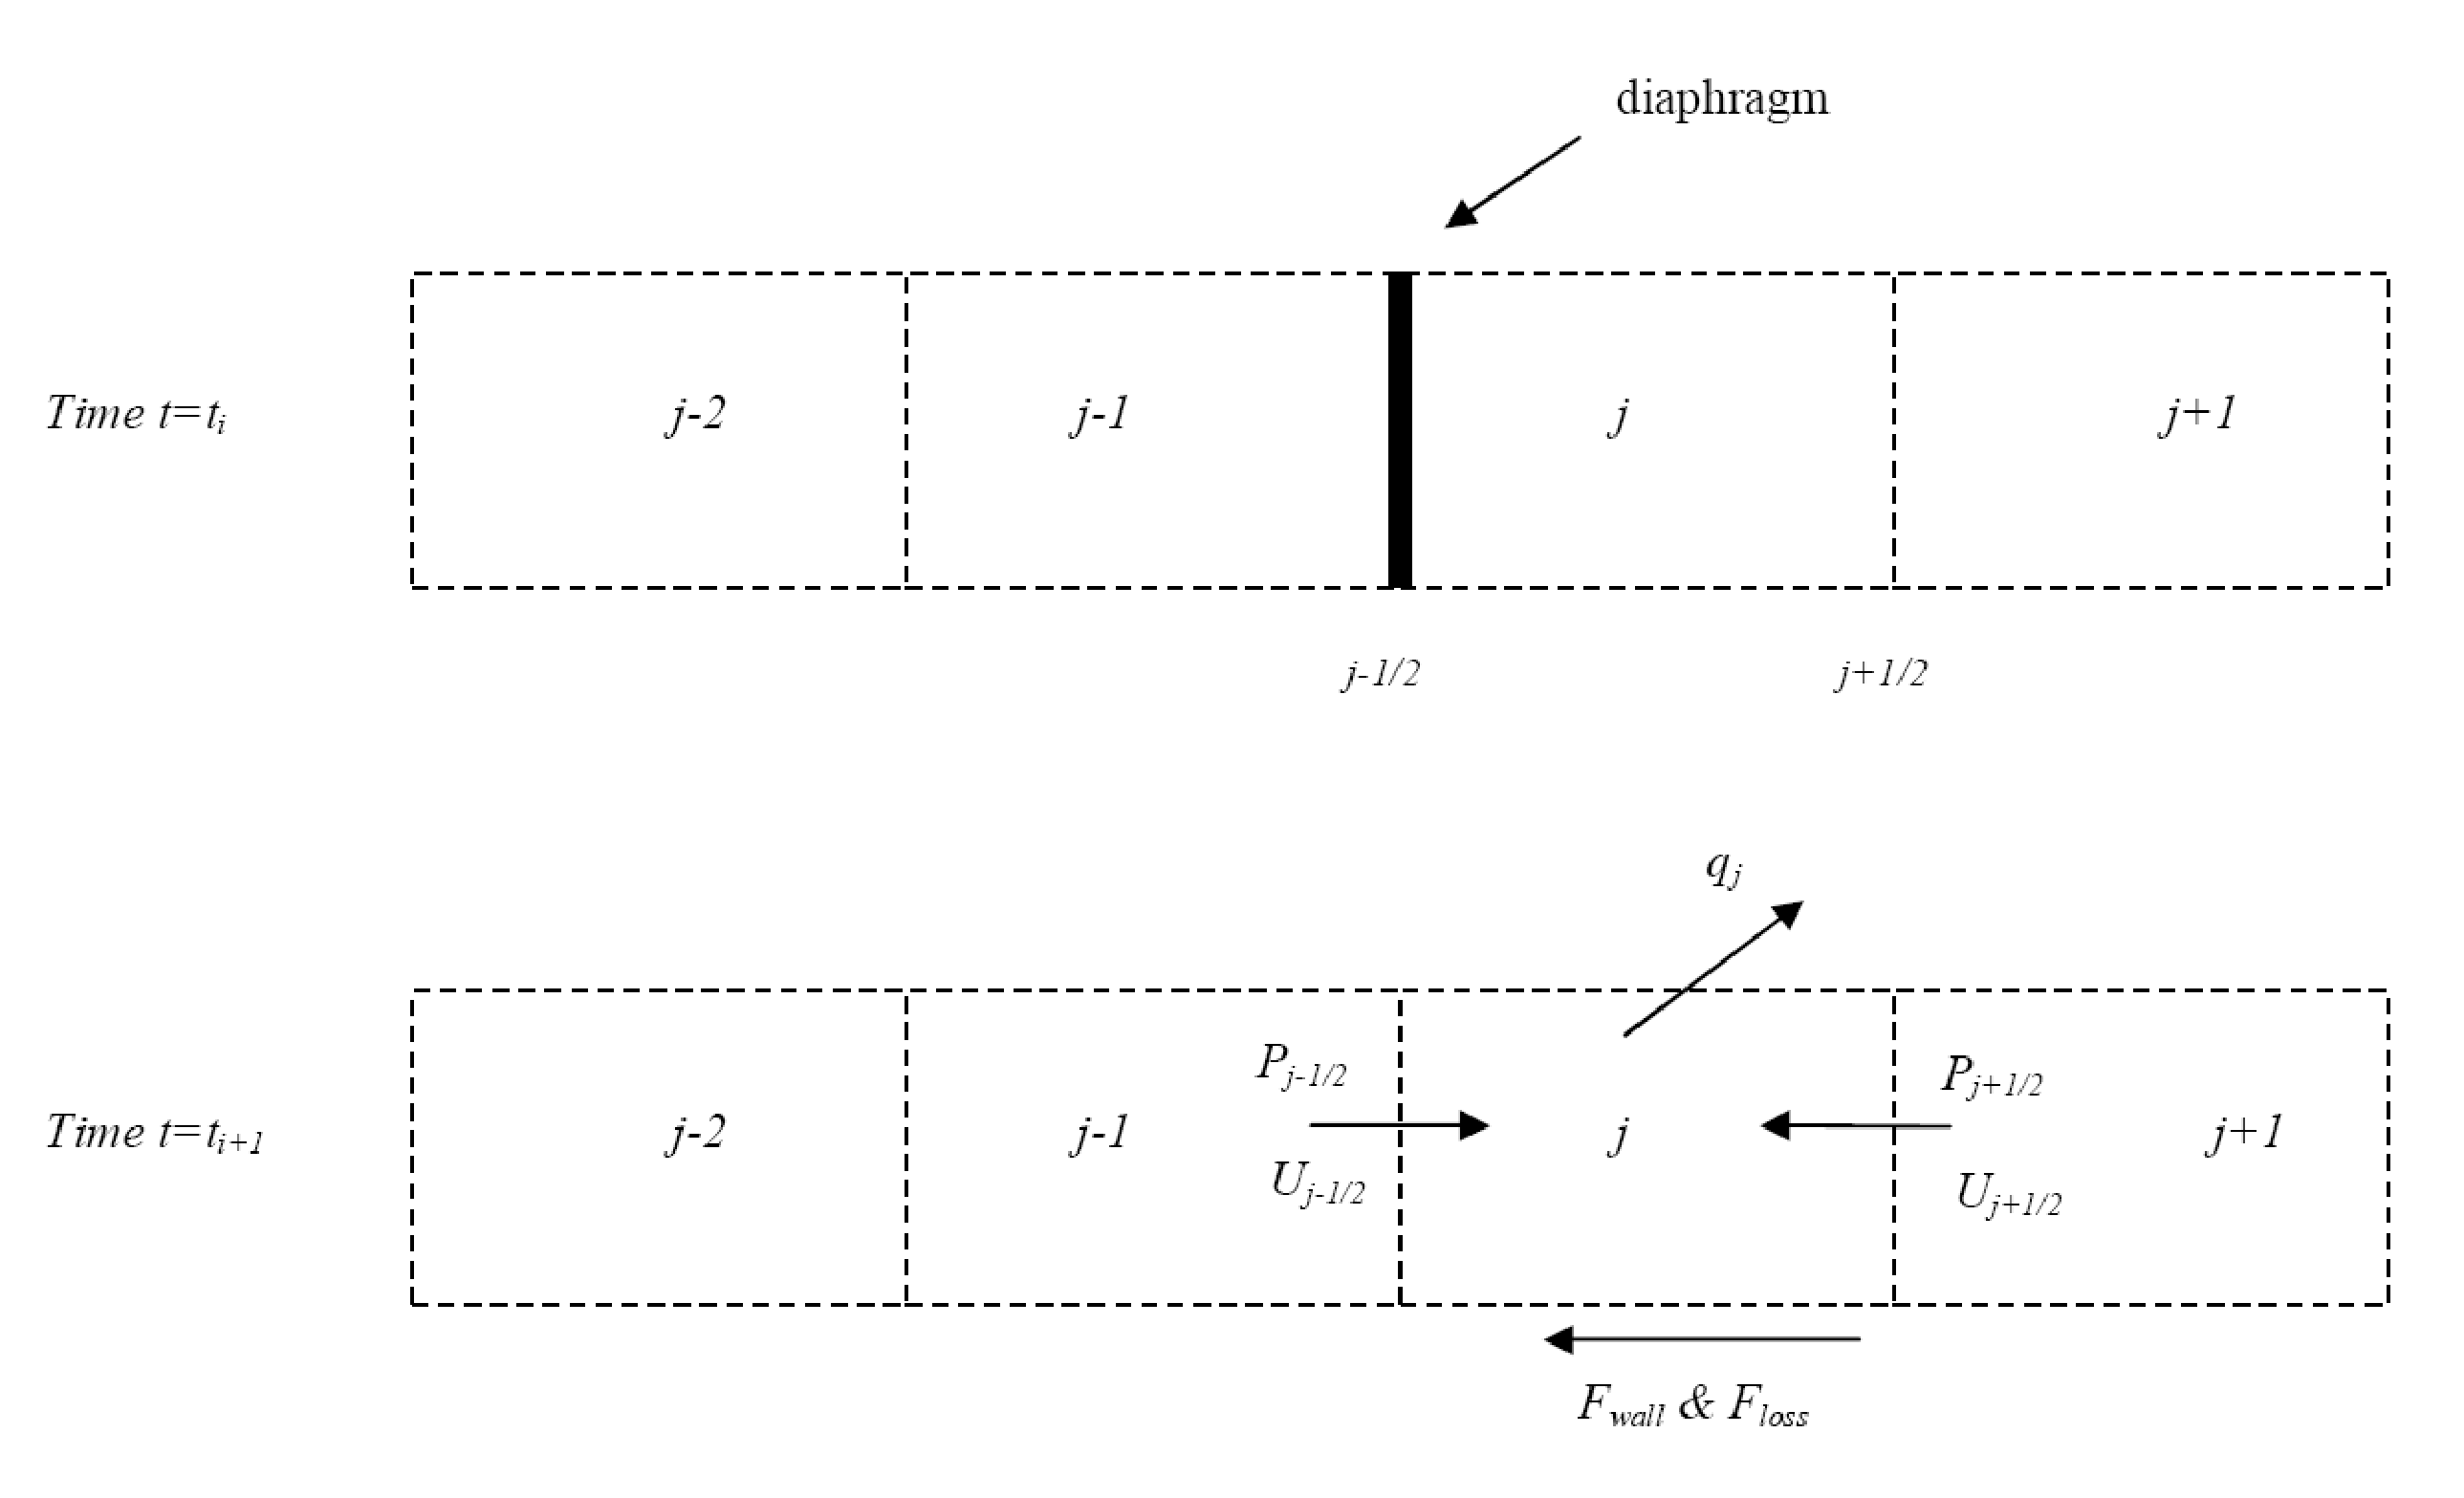
\includegraphics{figs/l1d_diaphragm.eps}}}
\caption{Flux terms immediately following rupture of light secondary or tertiary diaphragm in L1d} \label{1ld_diaphragm}
\end{figure}

\par

Such a scenario exists in L1d when a holding time diaphragm rupture model is implemented, \emph{Figure \ref{1ld_diaphragm}}.  Consider two cells either side of the secondary diaphragm at time $t_{j}$ just prior to rupture.  Where a hold time model is implemented, the gas in cell $j-1$ is stagnant and has a pressure in the order of $p_{j-1} = 10^{6}$ Pa and temperature of approximately $T_{j-1} = 10^{4}$ K.  The acceleration tube gas in cell $j$ is typically low pressure air of approximately 10 Pa and ambient temperature.  Assume that between time steps $t_{j}$ and $t_{j+1}$ the diaphragm hold time has elapsed, leaving the two cells $j-1$ and $j$ of different composition and flow state separated only by an interface.  The flux calculator in L1d, an approximate perfect gas Riemann solver, will solve for the interface velocity and pressure between the two cells, with the pressure being in the order of $10^4$ Pa and the velocity $10^4$ m/s.  The right hand side pressure velocity product is insignificant to that of the right, as is the heat loss term due to the low adiabatic wall temperature. The result is an unreasonably high energy flux to cell $j$, which manifests as a temperature in the order of $10^5$K for a time step of $\Delta t = 10^{-9} $.

\section{Inviscid flow profiles}
\label{appendix_B}

\subsection{9km/s Air condition}

\begin{figure}[h]
  \begin{center}
    \mbox{
      \subfigure[Pressure]
      {
         \label{fig:sub:k}
         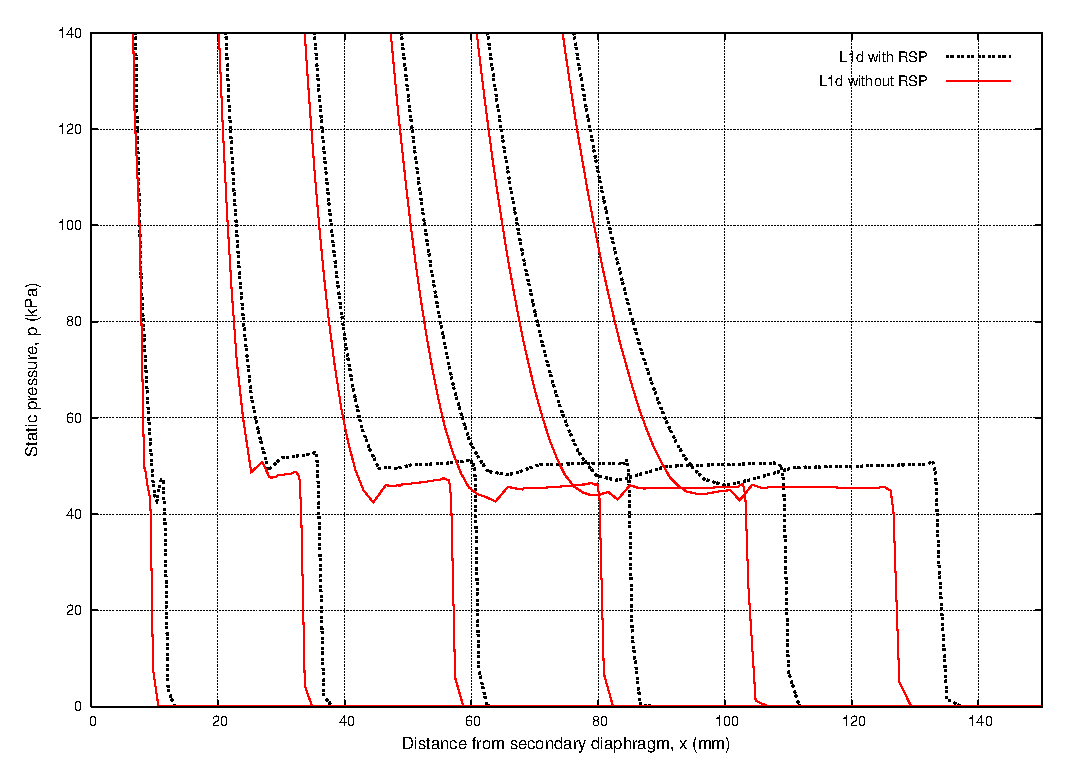
\includegraphics[scale=0.45]{figs/air_iv_press_profile.eps}
      } \quad
      \subfigure[Temperature]
      {
         \label{fig:sub:l}
         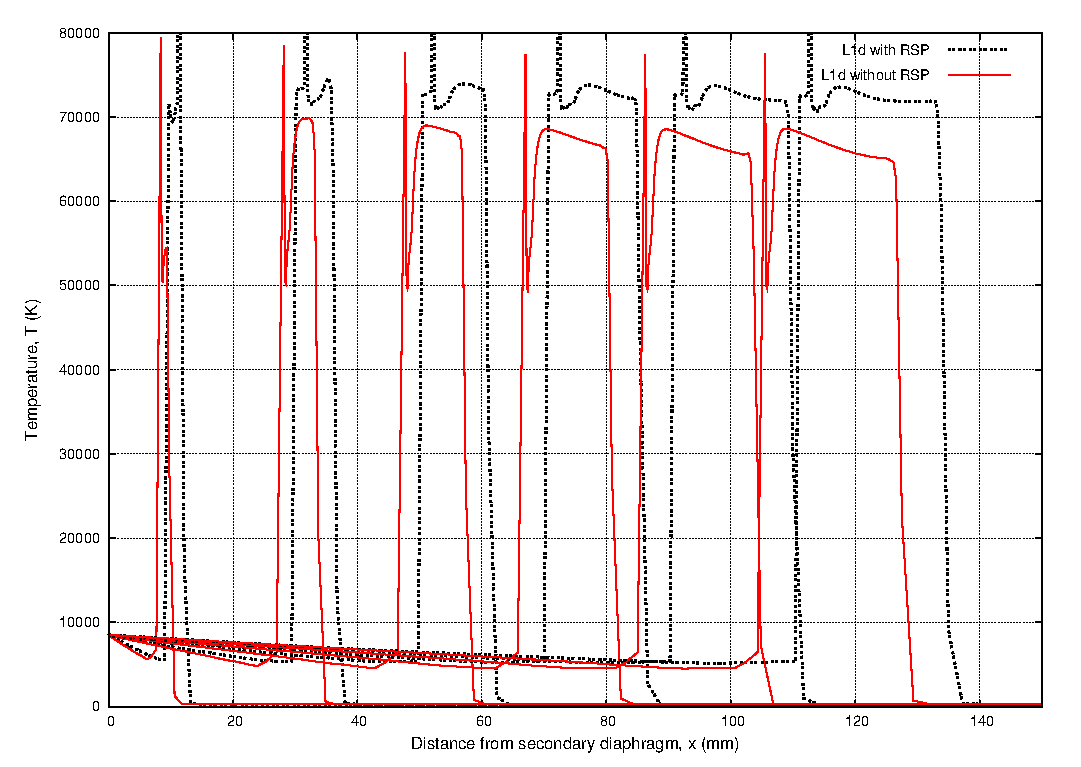
\includegraphics[scale=0.45]{figs/air_iv_temp_profile.eps}
      }
      }
    \mbox{
      \subfigure[Density]
      {
         \label{fig:sub:m}
         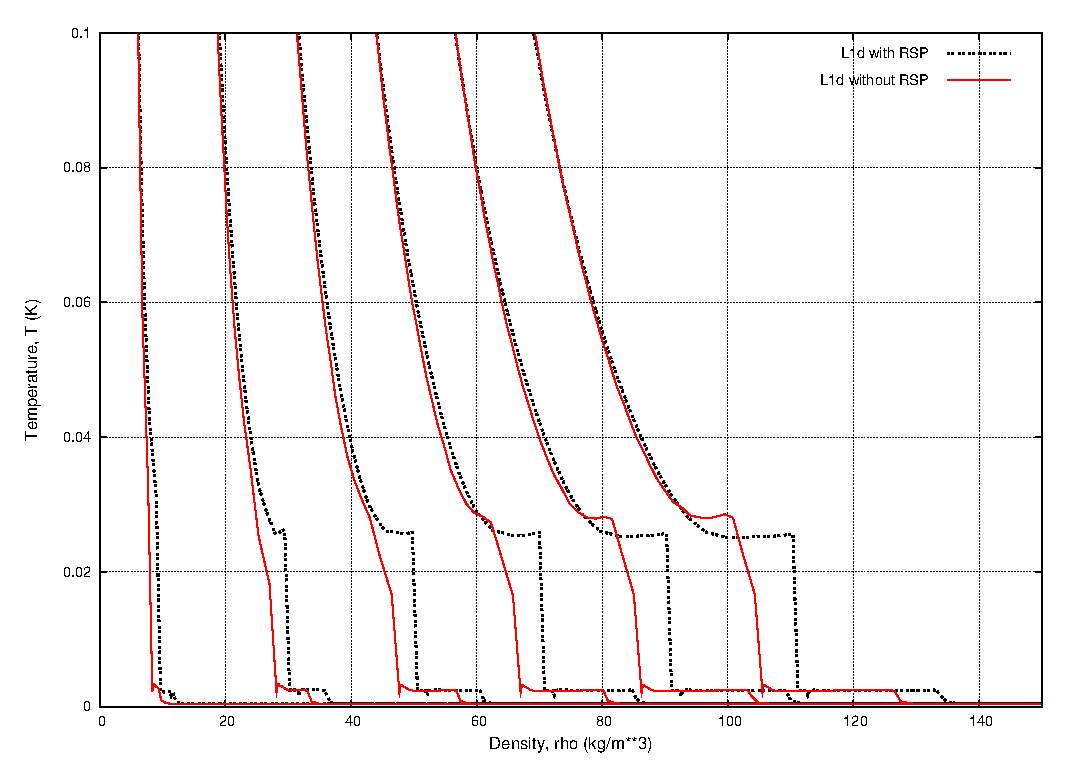
\includegraphics[scale=0.45]{figs/air_iv_density_profile.eps}
      } \quad
      \subfigure[Velocity]
      {
         \label{fig:sub:n}
         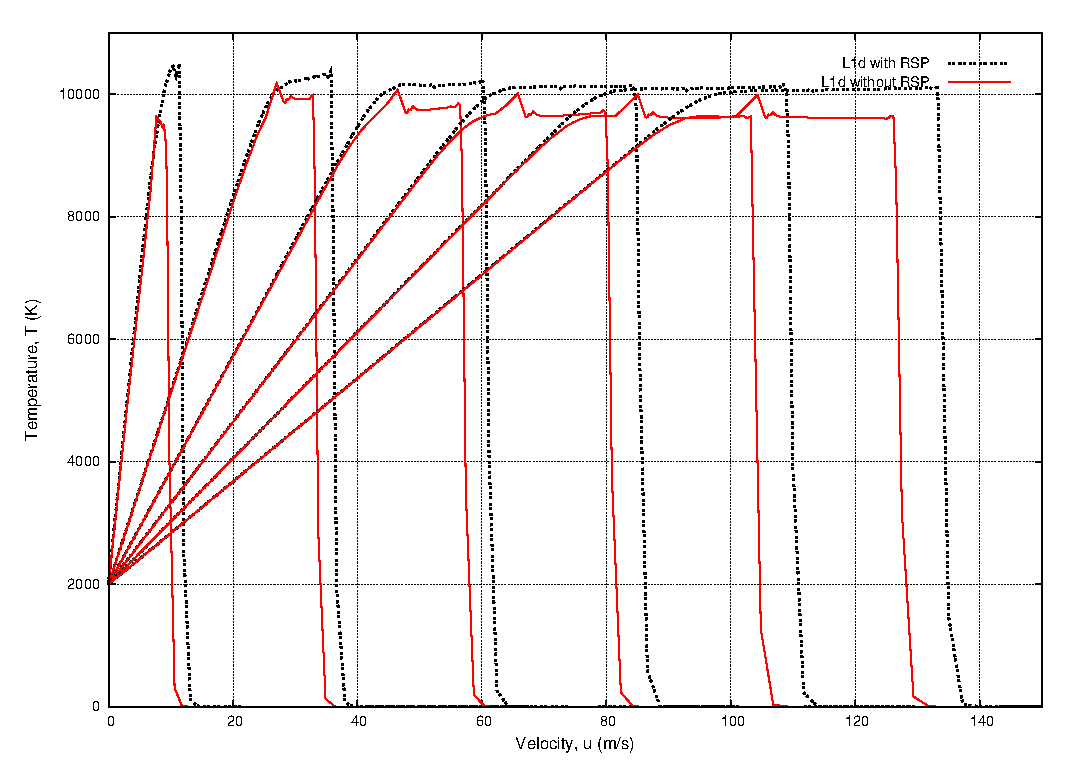
\includegraphics[scale=0.45]{figs/air_iv_velocity_profile.eps}
      } 
      }
    \caption{Inviscid L1d flow profiles for a 9km/s air condition in the X2 expansion tube with $t_{hold} = 10 \mu s$ and $\Delta t_{RSP} = 0.7 \mu $ (flow profiles for the first $10 \mu s$ after diaphragm rupture displayed)}
    \label{fig:mars_profiles}
  \end{center}
\end{figure}

\newpage

\subsection{6.6km/s Mars condition}

\begin{figure}[htbp]
  \begin{center}
    \mbox{
      \subfigure[Pressure]
      {
         \label{fig:sub:o}
         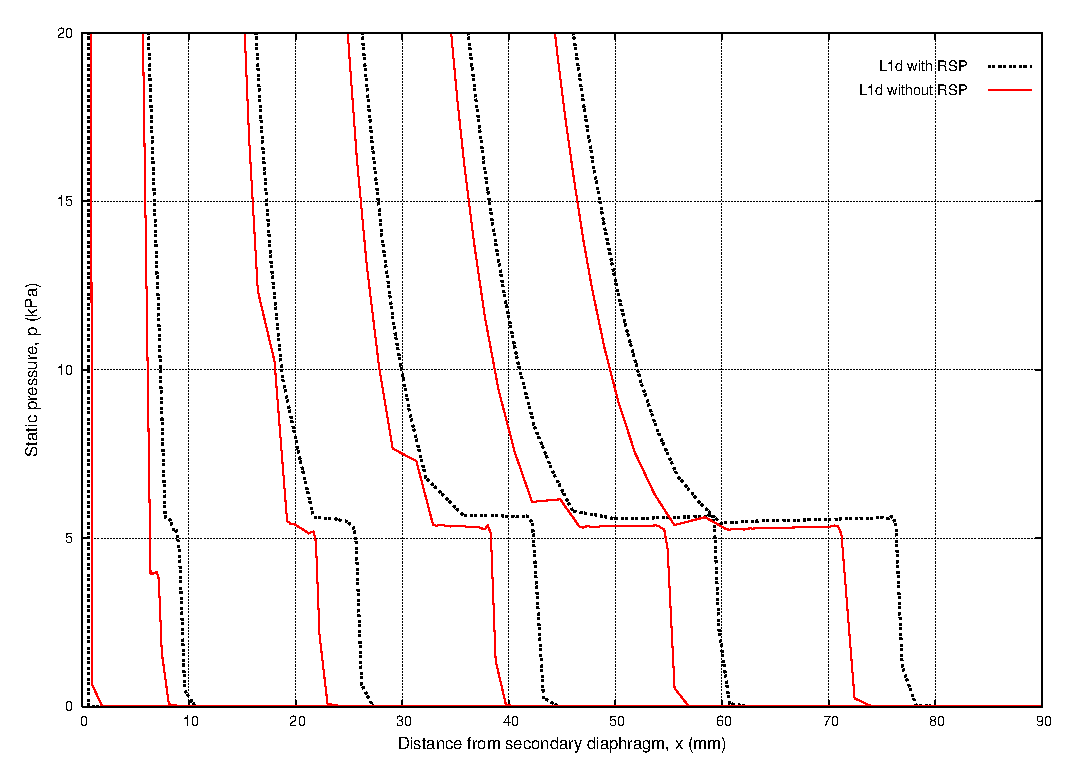
\includegraphics[scale=0.45]{figs/mars_iv_press_profile.eps}
      } \quad
      \subfigure[Temperature]
      {
         \label{fig:sub:p}
         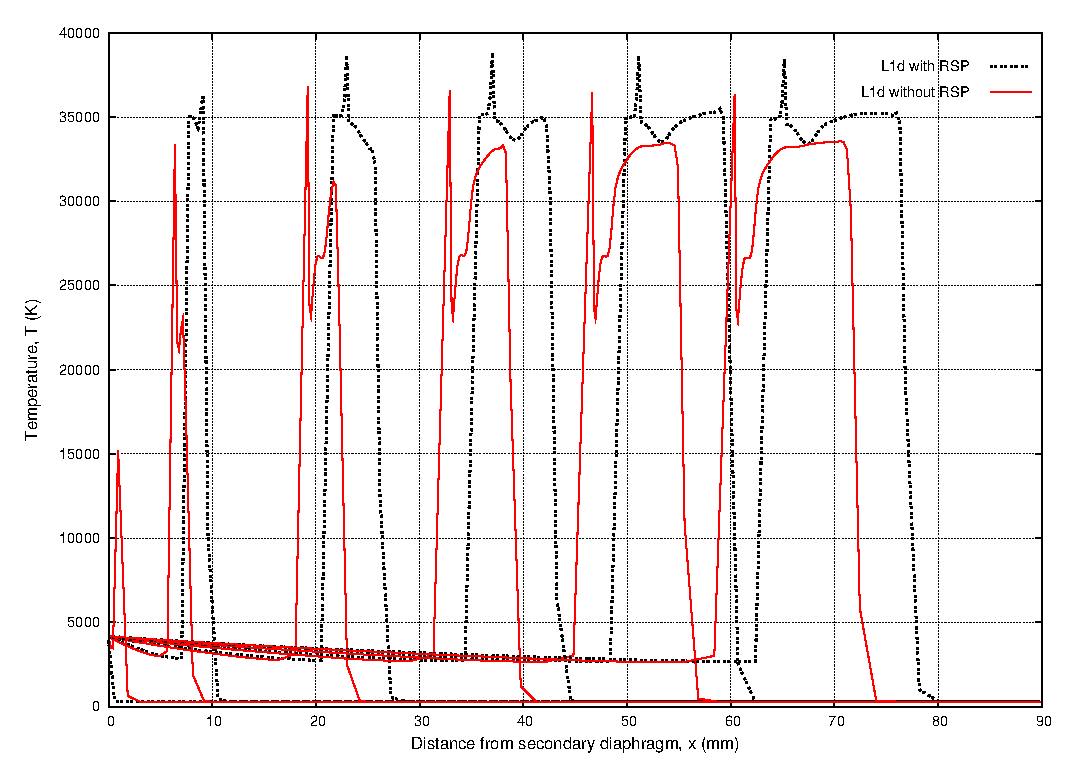
\includegraphics[scale=0.45]{figs/mars_iv_temp_profile.eps}
      }
      }
    \mbox{
      \subfigure[Density]
      {
         \label{fig:sub:q}
         \includegraphics[scale=0.45]{figs/mars_iv_density_profile.eps}
      } \quad
      \subfigure[Velocity]
      {
         \label{fig:sub:r}
         \includegraphics[scale=0.45]{figs/mars_iv_velocity_profile.eps}
      } 
      }
    \caption{Inviscid flow profiles for a 6.6km/s Mars gas condition in the X2 expansion tube}
    \label{fig:mars_profiles}
  \end{center}
\end{figure}

\newpage

\subsection{11km/s Jupiter condition}

\begin{figure}[htbp]
  \begin{center}
    \mbox{
      \subfigure[Pressure]
      {
         \label{fig:sub:k}
         \includegraphics[scale=0.45]{figs/jupiter_iv_press_profile.eps}
      } \quad
      \subfigure[Temperature]
      {
         \label{fig:sub:l}
         \includegraphics[scale=0.45]{figs/jupiter_iv_temp_profile.eps}
      }
      }
    \mbox{
      \subfigure[Density]
      {
         \label{fig:sub:m}
         \includegraphics[scale=0.45]{figs/jupiter_iv_dens_profile.eps}
      } \quad
      \subfigure[Velocity]
      {
         \label{fig:sub:n}
         \includegraphics[scale=0.45]{figs/jupiter_velocity_profile.eps}
      } 
      }
    \caption{Inviscid L1d flow profiles for a 11km/s Jupiter condition in the X2 expansion tube with $t_{hold} = 10 \mu s$ and $\Delta t_{RSP} = 0.4 \mu $ (flow profiles for the first $10 \mu s$ after diaphragm rupture displayed)}
    \label{fig:mars_profiles}
  \end{center}
\end{figure}


\end{document}          
